%\documentclass[utf8]{book}
\documentclass[10.5pt,a4paper]{ctexbook} % 五号字,A4


%========== 包 ==========
%\usepackage[UTF8]{ctex}                   % chinese
\usepackage{anyfontsize}                  % 10.5pt in ctexbook
\usepackage{booktabs}                     % \newpage
\usepackage{tcolorbox}                    % frame box
\usepackage{enumitem}                     % item
\usepackage{graphicx}                     % images
\usepackage{amsmath, amsthm, amssymb, bm} % math
\usepackage{hyperref, mathrsfs}           % ref
\usepackage{esint}                        % closed geometry integral symbol
\usepackage{pythonhighlight}              % Python code
\usepackage{appendix} % 引入appendix宏包


%========== 环境 ==========
\newtheorem{definition}{定义}[section]
\newtheorem{example}{例}[section]
\newtheorem{theorem}{定理}[section]
\newtheorem{lemma}[theorem]{引理}
\newtheorem{corollary}[theorem]{推论}
\newtheorem{proposition}[theorem]{命题}
\newtheorem{exercise}{习题}[chapter]


%========== enum和item设置 ==========
%\ctexset{section={beforeskip=50.0ex plus 0.2ex minus .2ex}}
%\ctexset{section={beforeskip=\doublespace}}
%\ctexset{section={format=\heiti\centering\zihao{-3},beforeskip=20cm},subsection={beforeskip=6ex}}
\ctexset{section={beforeskip=5ex},subsection={beforeskip=5ex}}
\setcounter{secnumdepth}{3}
\setcounter{tocdepth}{3}
\setenumerate[1]{itemsep=0pt,partopsep=0pt,parsep=\parskip,topsep=0pt,left=\parindent}
\setitemize[1]{itemsep=0pt,partopsep=0pt,parsep=\parskip,topsep=0pt,left=\parindent}
\setdescription{itemsep=0pt,partopsep=0pt,parsep=\parskip,topsep=5pt}
\graphicspath{{./figures}}


%========== 文档 ==========
\raggedbottom
\begin{document}


%========== 封面 ==========
\title{{\Huge{\textbf{信号与系统}}}\\——学习笔记}
\author{程琰}
\date{\today}
%\linespread{1.5}
\maketitle


% %========== 前言 ==========
% \newpage
% \pagenumbering{roman}
% \setcounter{page}{1}
% \begin{center}
%     \Huge\textbf{前言}
% \end{center}

% 这是笔记的前言部分。这是笔记的前言部分。这是笔记的前言部分。这是笔记的前言部分。这是笔记的前言部分。这是笔记的前言部分。这是笔记的前言部分。

% \begin{flushright}
%     \begin{tabular}{c}
%         程琰\\
%         \today
%     \end{tabular}
% \end{flushright}


%========== 目录 ==========
\newpage
\pagenumbering{Roman}
\setcounter{page}{1}
\tableofcontents


%========== 正文 ==========
\newpage
\setcounter{page}{1}
\pagenumbering{arabic}
\chapter{基本概念}

信号与系统的概念广泛存在于各个领域。
可以说,当今科技的发展离不开该理论的发展。
信号与系统这门学科就是将各个领域的问题抽象,用数学语言描述和分析,是介于数学和具体学科之间的一门科学。

本章介绍信号和系统的基本概念,并给出几个基本例子。

本章要点:
\begin{itemize}
    \item 信号和系统的概念。
    \item 基本信号:正弦、指数、阶跃、冲激。
    \item 系统的重要特性:线性、时不变、因果。
\end{itemize}

\newpage
\section{信号与系统概述}

本节介绍信号和系统的概念。

本节要点:
\begin{itemize}
    \item 掌握信号、系统及其相关概念。
\end{itemize}

%============================================================
\subsection{信号的概念}

\begin{definition}[信号]
在数学的角度,{\bf 信号}(signal)就是函数,自变量可以是时间、空间等,可以是一元函数,也可以是多元函数。
本书讨论的信号是以时间为自变量的一元函数,通常记为$x\left( t \right) $。
\end{definition}

物理意义上,信号指的是一个物体的状态。
若物体是一实物,则状态可以是物体的位移、速度。
若物体是一场,则状态可以是场强、电压、电流。
总之,信号描述的是一个物体的状态随时间的变化。

可以定义信号的{\bf 能量}和{\bf 功率}:
\begin{align*}
&E=\int_{t_1}^{t_2}{\left| x\left( t \right) \right|^2dt} \\
&P=\frac{1}{t_2-t_1}\int_{t_1}^{t_2}{\left| x\left( t \right) \right|^2dt}
\end{align*}
从能量和功率的角度,信号可以分有限能量信号$E_{\infty}<\infty $、有限功率信号$P_{\infty}<\infty $和能量功率均无限的信号。
而且易得,如果有限能量必然功率为0,如果有限功率必然能量无穷。

这个“功率”和“能量”是纯粹信号与系统上的概念。
虽然和具体物理意义无关,但还是有抽象层面的关系,如弹性势能$E=\frac{1}{2}kl^2$,动能$E=\frac{1}{2}mv^2$。

~

信号与系统中一个重要的概念就是信号的变换,对于以时间为自变量的信号指的就是时间轴的变换:
\begin{itemize}
    \item {\bf 时移}(time shift):$x\left( t-t_0 \right) $,表示信号延迟,或者波形右移。
    \item {\bf 尺变}(time scaling):$x\left( at \right) $,$a>1$表示信号变快,波形压缩,$a<1$表示信号变慢,波形伸长,$a=-1$表示信号{\bf 反转}(time reversal)。
    \item {\bf 周期}:若信号有$x\left( t+T \right) =x\left( t \right) $,则称为{\bf 周期信号}(periodic signal),最小正值$T$称为{\bf 基波周期}(fundamental period)。
    \item {\bf 奇偶性}:若信号有$x\left( t \right) =x\left( -t \right) $,称为{\bf 偶信号}(even),若$x\left( t \right) =-x\left( -t \right) $,称为{\bf 奇信号}(odd),易得,所有信号都可以分解为奇信号和偶信号的和:
    \begin{align*}
    &x_{even}\left( t \right) =\frac{1}{2}\left[ x\left( t \right) +x\left( -t \right) \right] \\
    &x_{odd}\left( t \right) =\frac{1}{2}\left[ x\left( t \right) -x\left( -t \right) \right]
    \end{align*}
\end{itemize}

\begin{tcolorbox}
注,$x\left( t \right) =C$是周期信号,但没有基波周期。
\end{tcolorbox}

%============================================================
\subsection{系统和响应的概念}

\begin{definition}[系统]
{\bf 系统}(system)是组件与端口的互连,通过这些端口可以输出输入信息。
\end{definition}

我们称一组描述输入输出之间相互关系的数学方程为{\bf 系统的数学模型}(mathematical model)。
数学模型是一种描述系统的数学工具,好的数学模型是需要在精确性和简单性之有良好的平衡,两大基本数学模型:
\begin{itemize}
    \item {\bf 输入输出模型}(input/output model):描述输入信号和输出信号之间关系,具体分:
    \begin{itemize}
        \item {\bf 微分方程}(differential equation)和{\bf 差分方程}(difference equation),
        \item {\bf 卷积模型}(convolution model),
        \item {\bf 傅里叶变换}(Fourier transform),
        \item {\bf 传递函数}(transfer function);
    \end{itemize}
    \item {\bf 状态模型}(state model):描述输入、状态、输出之间关系。
\end{itemize}
其中,傅里叶变换可视为传递函数的一个特例。

\begin{definition}[响应]
对于一个特定的输入或系统本身状态,系统会产生一个特定的输出,称为{\bf 响应}(response)。根据引起响应的不同原因,响应可以分为:
\begin{itemize}
    \item {\bf 零输入响应}(zero input):系统响应仅由其初始状态引起,输入始终为0;
    \item {\bf 零状态响应}(zero state):系统初始状态为0,响应仅由输入引发。
\end{itemize}
\end{definition}

\begin{tcolorbox}
为简化讨论,本笔记讨论只有一个输入和一个输出的系统,且系统默认都是零状态响应。
\end{tcolorbox}









\newpage
\section{连续信号}

本节介绍连续信号,并给出4种基本的连续信号。

本节要点:
\begin{itemize}
    \item 掌握连续信号的概念;
    \item 熟悉4个基本连续信号。
\end{itemize}

%============================================================
\subsection{连续信号的概念}

\begin{definition}[连续信号]
当时间变量$t$取值实数时,我们称信号为{\bf 连续信号}(continuous-time signal)或{\bf 模拟信号}(analog signal),通常记为$x\left( t \right) $。
\end{definition}

%============================================================
\subsection{正弦信号}

\[
x\left( t \right) =A\sin \left( \omega t+\varphi \right)
\]
\begin{itemize}
    \item $A$:振幅;
    \item $\omega $:角频;
    \item $\varphi $:相位。
\end{itemize}
周期和频率:
\[
T=\frac{2\pi}{\omega} \qquad f=\frac{1}{T}=\frac{\omega}{2\pi} \qquad \omega =2\pi f
\]

%============================================================
\subsection{指数信号}

\[
x\left( t \right) =Ae^{at}
\]

当$a$为实数,信号的定义域和值域都是实数,称为{\bf 实指数信号}。
当$a>0$时,信号发散,如原子弹爆炸;当$a<0$时,信号衰减;当$a=0$时,信号为常数。
在实际系统中,一般信号都是衰减信号,所以写成:
\[
x\left( t \right) =Ae^{-\frac{t}{\tau}} \qquad \tau >0,t\geqslant 0
\]
其中,$\tau $称为{\bf 时间常数},反映了信号的衰减速度。

\begin{tcolorbox}
曲线$x\left( t \right) =Ae^{-\frac{t}{\tau}}$过曲线上点$\left( t_0,Ae^{-\frac{t_0}{\tau}} \right) $的切线方程:
\[
x\left( t \right) -Ae^{-\frac{t_0}{\tau}}=-\frac{A}{\tau}e^{-\frac{t_0}{\tau}}\left( t-t_0 \right)
\]
交于{\it t}轴:
\begin{align*}
&\because -Ae^{-\frac{t_0}{\tau}}=-\frac{A}{\tau}e^{-\frac{t_0}{\tau}}\left( t-t_0 \right) \\
&\therefore t=t_0+\tau
\end{align*}
这里可以得到衰减的实指数信号的一个特征,曲线切线与{\it t}轴的交点和切点的时间差永远是$\tau $。
\end{tcolorbox}

当$a$为复数$s=\sigma +i\omega $时信号为:
\[
x\left( t \right) =Ae^{st}
\]
此时信号的值域都是复数,称为{\bf 复指数信号},模、实部和虚部如下:
\begin{align*}
&\left| x\left( t \right) \right|=Ae^{\sigma t} \\
&\mathrm{Re}\left[ x\left( t \right) \right] =Ae^{\sigma t}\mathrm{Re}\left[ e^{i\omega t} \right] =Ae^{\sigma t}\cdot \cos \left( \omega t \right) \\
&\mathrm{Im}\left[ x\left( t \right) \right] =Ae^{\sigma t}\mathrm{Im}\left[ e^{i\omega t} \right] =Ae^{\sigma t}\cdot \sin \left( \omega t \right)
\end{align*}
实部和虚部都是正弦信号,且$T=2\pi /\omega $,两者“对称”振荡,整体由指数包络。
$\sigma $决定发散还是衰减,系统能量:
\[
E_{\infty}=\int_0^{+\infty}{\left| Ae^{st} \right|^2dt}=A^2\int_0^{+\infty}{e^{2\sigma t}dt}=\frac{A^2}{2\sigma}\left( \left. e^{2\sigma t} \right|_{0}^{+\infty} \right)
\]
当时$\sigma <0$,信号是有限能量。

物理中,复指数较实指数更为普遍。复指数代表着两个状态或者两种能量的相互转化,如弹簧的简谐振动、RC振荡电路。
$\omega $决定了转化速度,$\sigma $决定了系统是否对外辐射能量。
所以在复指数中,一个变量$s=\sigma +i\omega $就表示了系统的内在运动和对外关系。

当$s$为纯虚数时,写为:
\[
x\left( t \right) =Ae^{i\omega t}=A\left( \cos \omega t+i\sin \omega t \right)
\]
称为{\bf 纯虚指数信号}。
只有当$s$为纯虚数时,信号才是周期信号。
纯虚指数信号另一个特征是有限功率:
\[
P_{\infty}=\underset{T\rightarrow \infty}\lim \frac{1}{T}\int_{-\frac{T}{2}}^{\frac{T}{2}}{\left| Ae^{i\omega t} \right|^2dt}=\underset{T\rightarrow \infty}\lim \frac{1}{T}\int_{-\frac{T}{2}}^{\frac{T}{2}}{A^2dt}=A^2
\]

如果一个信号是纯虚指数信号,表示系统对外没有能量交换,如无阻尼谐振子。

%============================================================
\subsection{单位阶跃和单位冲激}

\begin{figure}[h]
\centering
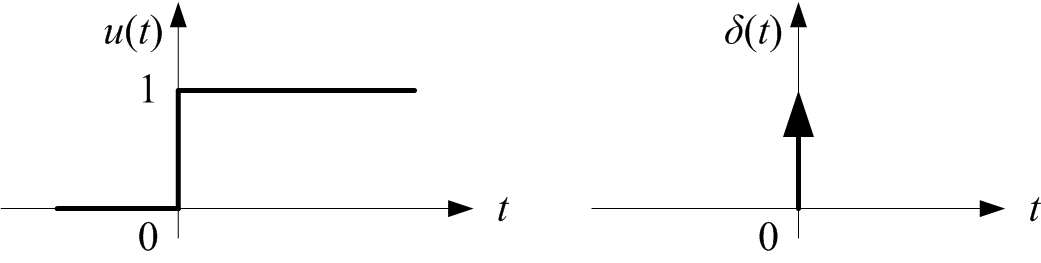
\includegraphics[height=2cm]{1.2.4-1.png}
\end{figure}
\[
u\left( t \right) =\begin{cases}
	1 \quad t\geqslant 0\\
	0 \quad t<0\\
\end{cases} \qquad \begin{array}{l}
	\delta \left( t \right) =0 \quad t\ne 0\\
	\int_{-\infty}^{+\infty}{\delta \left( \tau \right) d\tau}=1\\
\end{array}
\]
两者关系:
\[
\begin{cases}
	u\left( t \right) =\int_{-\infty}^t{\delta \left( \tau \right) d\tau}\\
	\delta \left( t \right) =\frac{du\left( t \right)}{dt}\\
\end{cases}
\]
严格来讲,因为$u\left( t \right) $在$t=0$不连续,所以$\delta \left( t \right) $不是$t=0$的导数。
但不妨碍讨论。

从$u\left( t \right) =\int_{-\infty}^t{\delta \left( \tau \right) d\tau}$来看,$u\left( t \right) $是$\delta \left( t \right) $的积分上限函数,即是积分区间的移动。
令$\tau =t-\sigma $,有:
\begin{align*}
&d\tau =d\left( t-\sigma \right) =-d\sigma \\
&u\left( t \right) =\int_{-\infty}^t{\delta \left( \tau \right) d\tau}=-\int_0^{+\infty}{\delta \left( t-\sigma \right) d\sigma}
\end{align*}
可以认为积分区间不动,$u\left( t \right) $是$\delta \left( t \right) $的移动的结果。
\begin{figure}[h]
\centering
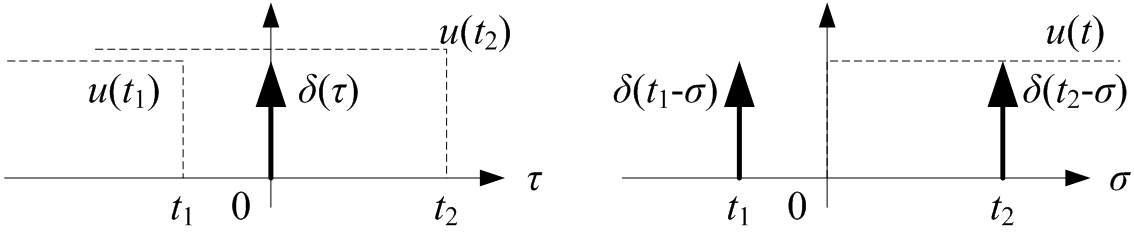
\includegraphics[height=2cm]{1.2.4-2.png}
\end{figure}

$\delta \left( t \right) $的特征:
\begin{itemize}
    \item 偶函数,$\delta \left( t \right) =\delta \left( -t \right) $。
    \item 单位面积,$\int_{-\infty}^{+\infty}{\delta \left( \tau \right) d\tau}=1$,也即能量有限。
    \item 尺度变换性质,$\delta \left( at \right) =\frac{1}{\left| a \right|}\delta \left( t \right) $。
    \item 筛选性,$f\left( t \right) =\int_{-\infty}^{+\infty}{f\left( t \right) \delta \left( \tau -t \right) d\tau}$。
\end{itemize}

$\delta \left( t \right) $的导数:将两个“微小错开”的正负单位冲激的叠加称为{\bf 单位冲激偶},记为$\delta '\left( t \right) $,有如下特征:
\begin{itemize}
    \item 奇函数,$\delta '\left( t \right) =-\delta '\left( -t \right) $。
    \item 面积为0,$\int_{-\infty}^{+\infty}{\delta '\left( \tau \right) d\tau}=0$,也即无能量。
    \item 筛选性,$\int_{-\infty}^{+\infty}{f\left( t \right) \delta '\left( \tau -t \right) d\tau}=-f'\left( t \right) $。
\end{itemize}

%============================================================
\subsection{广义导数}

\begin{definition}[广义导数]
假设信号$x\left( t \right) $在$t_0$不可导,我们定义$x\left( t \right) $在$t_0$的{\bf 广义导数}(generalized derivative)为:
\[
\left. \frac{dx\left( t \right)}{dt} \right|_{t=t_0}=\left[ x\left( {t_0}^+ \right) -x\left( {t_0}^- \right) \right] \delta \left( t-t_0 \right)
\]
即用冲激函数筛选$\left[ x\left( {t_0}^+ \right) -x\left( {t_0}^- \right) \right] \delta \left( t-t_0 \right) $代替$t_0$处的导数。
\end{definition}






\newpage
\section{离散信号}

本节介绍离散信号,并给出2种基本的离散信号。

本节要点:
\begin{itemize}
    \item 掌握离散信号的概念;
    \item 熟悉2个基本离散信号。
\end{itemize}

%============================================================
\subsection{离散信号的概念}

\begin{definition}[离散信号]
当时间变量取离散值$t=t_n,n=0,\pm 0,\pm 2,\cdots $时,我们称信号为{\bf 离散信号}(discrete-time signal),记为$x\left[ n \right] $,其中$n$表示$t_n$,即第$n$个时间采样点。
一般我们通过对连续信号的周期性采样获得离散信号,即:
\begin{align*}
&n=\frac{t}{T} \\
&x\left[ n \right] =\left. x\left( t \right) \right|_{t=nT}=x\left( nT \right)
\end{align*}
其中,$T$为采样周期,单位s。
\end{definition}

虽然不硬性规定$t_n$之间的间隔,但一般我们还是等间隔处理,即“周期性”采样。

%============================================================
\subsection{单位阶跃和单位冲激}

\begin{figure}[h]
\centering
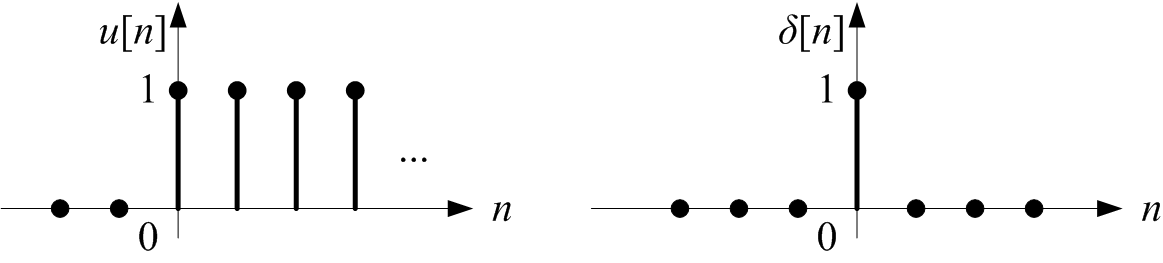
\includegraphics[height=2cm]{1.3.2-1.png}
\end{figure}
\[
u\left[ n \right] =\begin{cases}
	1 \quad n=0,1,2,\cdots\\
	0 \quad n=-1,-2,\cdots\\
\end{cases} \quad \delta \left[ n \right] =\begin{cases}
	1 \quad n=0\\
	0 \quad n=\pm 1,\pm 2,\cdots\\
\end{cases}
\]






\newpage
\section{系统的特性}

本节介绍系统的4大特性。

本节要点:
\begin{itemize}
    \item 掌握系统的4大特性:线性性,时不变,因果性,有限维度。
\end{itemize}

\begin{tcolorbox}
本书讨论的系统,都符合这4大特性。
\end{tcolorbox}

%============================================================
\subsection{线性和时不变}

若系统满足:
\begin{itemize}
    \item $x_1\left( t \right) +x_2\left( t \right) \rightarrow y_1\left( t \right) +y_2\left( t \right) $:称为{\bf 可加的}(additive),
    \item $ax\left( t \right) \rightarrow ay\left( t \right) $:称为{\bf 均匀的},或{\bf 齐次的}(homogeneous)。
\end{itemize}
若都满足,称为{\bf 线性的}(linear)。
严格来讲,讨论线性时,对系统的要求是无初始状态,即零状态。
若系统满足$x\left( t-t_0 \right) \rightarrow y\left( t-t_0 \right) $,称为{\bf 时不变}(time invariant)。
时不变表示系统的特性不随时间变化而变化,如RC电路,短时间看是一个时不变系统。
但长时间看,由于电容电解液的消耗导致电容值发生改变,是一个时变系统。

线性和时不变是系统最重要的两个特性。
如果系统满足线性和时不变,则称为{\bf LTI系统},这样的系统在计算上可以大大简化。
绝大多数自然界系统也都可以认为是LTI系统。
信号与系统这门学科着重研究的就是LTI系统的表述和分析,如何将一个系统建模成LTI,即便无法建模成LTI,那如何近似成一个LTI。

%============================================================
\subsection{记忆和因果}

若输出只与该时刻和之前的输入有关,称系统为{\bf 因果系统}(casual system)。
若系统的输出只取决于当刻的输入,则称为{\bf 无记忆系统}(memoryless system),如电阻,反之,称为{\bf 有记忆系统}(system with memory),如电容。
实际系统中,记忆是直接和能量相联系的,比如电容存储的电荷,车辆保有的动能。
无记忆系统都是因果系统。

能量在系统内部会有某种“惯性”,使得信号在系统内部造成“回响”效果,系统的输出就是之前各个时间点的回响的“混响”效应:
\[
y\left[ n \right] =\sum_{i=-\infty}^n{a_ix\left[ i \right]}=a_nx\left[ n \right] +\sum_{i=-\infty}^{n-1}{a_ix\left[ i \right]}=a_nx\left[ n \right] +y\left[ n-1 \right]
\]
这就是差分(同理也是微分)的由来。
时域模型就是研究系统的回响和混响。

%============================================================
\subsection{有限维度}

若系统的输入输出关系可以用微分方程
\[
y^{\left( n \right)}\left( t \right) = f\left[ y\left( t \right) ,y'\left( t \right) ,\cdots ,y^{\left( n-1 \right)}\left( t \right) , x\left( t \right) ,x'\left( t \right) ,\cdots ,x^{\left( m \right)}\left( t \right) ,t \right]
\]
描述,则称为{\bf 有限维度系统}(finite dimensional system),$n$为系统的{\bf 维度}(dimension)或{\bf 阶}(order)。
特别地,当有限维度系统可以描述为
\[
y^{\left( n \right)}\left( t \right) +\sum_{i=0}^{n-1}{a_i\left( t \right) y^{\left( i \right)}\left( t \right)}=\sum_{i=0}^m{b_i\left( t \right) x^{\left( i \right)}\left( t \right)}
\]
即为{\bf 线性系统}。
若更进一步,当输入输出的系数为常数,即
\[
y^{\left( n \right)}\left( t \right) +\sum_{i=0}^{n-1}{A_iy^{\left( i \right)}\left( t \right)}=\sum_{i=0}^m{B_ix^{\left( i \right)}\left( t \right)}
\]
时,为{\bf 线性时不变系统}。

对于离散系统,若输入输出满足差分方程
\[
y\left[ n \right] = f\left( y\left[ n-1 \right] ,\cdots ,y\left[ n-N \right] ,x\left[ n \right] ,x\left[ n-1 \right] ,\cdots ,x\left[ n-M \right] ,n \right)
\]
称为{\bf 有限维度系统}(finite dimensional system),同样地,$N$称为系统的{\bf 维度}(dimension)或{\bf 阶}(order)。

%============================================================
\subsection{其他特性}

系统的其他特性还包括{\bf 可逆性}。
如编码系统,必须是可逆的,必有且仅有一个与之对应的逆系统进行解码。
如果系统在一个有限的输入下,响应收敛,称为{\bf 稳定的}。
一般来讲稳定性是由于能量消耗的原因。






\newpage
\section{例}

本节以4个实例介绍系统的概念,并给出其时域模型。

%============================================================
\subsection{RC电路}

\begin{example}
如下RC电路,假设电压源为系统输入信号$x\left( t \right) $,电容两端电压看作系统输出信号$y\left( t \right) $,试写出输入输出的微分方程。
\end{example}

\begin{figure}[h]
\centering
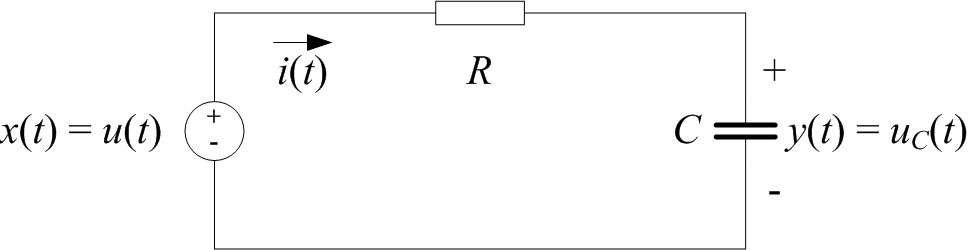
\includegraphics[height=2cm]{1.5.1-1.png}
\end{figure}

根据KVL推导RC电路的输入输出模型:
\begin{align*}
&\because u_C+u_R=u \\
&\therefore y+C\frac{dy}{dt}\cdot R=x \\
&\therefore \frac{dy}{dt}+\frac{1}{RC}y=\frac{1}{RC}x
\end{align*}
只要确定了输入信号$x=u\left( t \right) $,就可通过求解微分方程得到输出信号$y=u_C\left( t \right) $。

\begin{tcolorbox}
该RC电路会在之后的章节中反复讨论。
\end{tcolorbox}

%============================================================
\subsection{汽车运行}

\begin{example}
假设车辆在不光滑路面沿直线行驶,整个车辆作为系统,将发动机的动力视为系统输入$x$,行驶距离视为输出$y$,试写出系统的输入输出的微分方程。
\end{example}

根据牛顿定律我们可以得到车辆的加速度和受力的关系式:
\[
F=Ma
\]
车辆受力除了发动机的输出力之外,还有地面的摩擦力,摩擦力和速度成正比$K$,反向于速度方向,于是:
\[
x-K\frac{dy}{dt}=M\frac{d^2y}{dt^2}
\]
该微分方程即为车辆系统的微分方程。

%============================================================
\subsection{弹簧减震系统}

\begin{example}
如下图,系统由压块(质量$M$)、弹簧(胡克系数$K$)和阻尼器(阻尼系数$D$)组成,将压块受到的外力视为输入$x=F\left( t \right) $,压块位移视为输出$y=S\left( t \right) $,试写出输入输出的微分方程。
\end{example}

\begin{figure}[h]
\centering
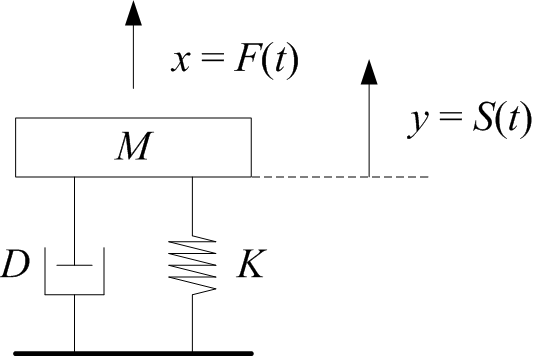
\includegraphics[height=3cm]{1.5.3-1.png}
\end{figure}

依然根据牛顿定律,考察压块的加速度和受力,弹簧施加反向作用力(大小和压块位移成正比),阻尼器施加反向作用力(大小和压块速度成正比),有:
\[
x-D\frac{dy}{dt}-Ky=M\frac{d^2y}{dt^2}
\]

%============================================================
\subsection{钟摆}

\begin{example}
假设有钟摆,输入为小球受的切向于运动方向的力$x=F\left( t \right) $,输出为偏转角$y=\theta \left( t \right) $,试写出输入输出的微分方程。
\end{example}

\begin{figure}[h]
\centering
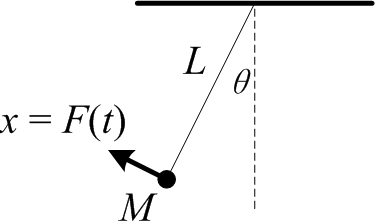
\includegraphics[height=2cm]{1.5.4-1.png}
\end{figure}

小球转动惯量为$I=ML^2$,收到两个外力$x=F\left( t \right) $和重力,它们产生的力矩分别为$xL,MgL\sin y$,根据牛顿定律对转动角加速度和力矩的关系,有:
\[
ML^2\cdot \frac{d^2y}{dt^2}=xL-MgL\sin y
\]
根据这个输入输出模型的描述,系统不是一个线性系统,无法得到解析解。
但是如果考虑偏转角很小$\sin \theta =\theta $有:
\[
ML\cdot \frac{d^2y}{dt^2}=x-Mg\cdot y
\]
变成了线性系统。
通过这样的处理后的系统称为{\bf 小信号系统}(small-signal system)。

\begin{tcolorbox}
有的时候,严格来讲,碰到的系统并不是LTI。
但是考虑到输入输出信号很小的情况下,可以近似用线性模型描述,这样的模型称为该系统的小信号模型。
在一定程度下,可以用一个简单的微分方程代替一个复杂的微分方程来考察系统。
\end{tcolorbox}






\newpage
\section{本章小结}

本章初步定义了一些信号与系统的概念,并举了几个例子。
这些例子涵盖不同的学科,但它们有一个共同的特点,一个输入量通过一个系统的作用产生一个输出量。

\begin{figure}[h]
\centering
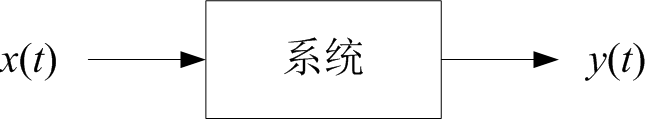
\includegraphics[height=1cm]{1.6-1.png}
\end{figure}

RC电路例子需要特别注意,在今后章节会反复引用。
\begin{figure}[h]
\centering
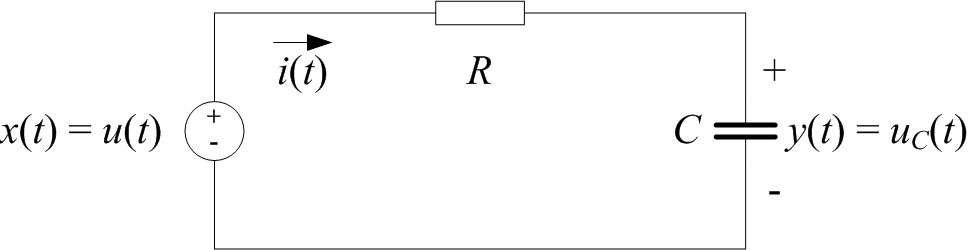
\includegraphics[height=2cm]{1.5.1-1.png}
\end{figure}
\[
\frac{dy}{dt}+\frac{1}{RC}y=\frac{1}{RC}x
\]










\chapter{微分方程和差分方程}

微分方程和差分方程是在时域描述系统的典型方法。
本章讲述微分方程、差分方程和通过欧拉近似将微分方程转为差分方程求得数值解。

微分方程是描述系统的最基础的方法,直接由物理公式推导得到,也是最接近物理本质的方法。
差分方程可以理解为一种求解微分方程数值解的方法。

本章要点:
\begin{itemize}
    \item LTI系统的微分方程。
    \item LTI系统的差分方程。
    \item 微分方程的离散化。
\end{itemize}

\newpage
\section{LTI系统的微分方程模型}

很多物理系统,如电路、钟摆、悬挂等,其变量间存在导数和积分关系,整个系统可用微分方程描述,所以微分方程模型关键在于建模和求解微分方程。

本节要点:
\begin{itemize}
    \item 掌握微分方程的概念;
    \item 掌握一阶常系数线性微分方程的求解思路。
\end{itemize}

%============================================================
\subsection{微分方程的概述}

若LTI系统是有限维度,则可以用线性常系数微分方程描述如下:
\[
y^{\left( n \right)}\left( t \right) +\sum_{i=0}^{n-1}{A_iy^{\left( i \right)}\left( t \right)}=\sum_{i=0}^m{B_ix^{\left( i \right)}\left( t \right)}
\]
其中,$A_i,B_i$是实数,$n$称为{\bf 系统的阶}(order)。
配合初始条件,即可求出输入输出的对应关系。
特别地,我们称
\[
y\left( t \right) =B_0x\left( t \right)
\]
这样的系统为{\bf 静态系统},即输出只与当刻的输入有关。
静态系统过于简单,不予讨论。
如果系统的输出不仅与当刻输入有关,更与前刻输入有关,则称为{\bf 动态系统},动态系统的时域模型必为微分方程。
通常简单的微分方程可以求解,复杂的方程非常难解,特别是高阶的,甚至没有解析解。

一般来讲,真实系统多多少少都会将输入信号的能量在系统内部有暂留,相当于输出的能量在系统内部“来回振荡”了几下叠合起来再输出,所以在时域模型上,都会体现成微分方程,至少是一阶。

%============================================================
\subsection{一阶常系数线性方程的求解}

\begin{tcolorbox}
为了方便求解,时域分析(本章和下一章的卷积)的大量例子都是以一阶微分方程为例,所以这里特别讨论一阶常系数线性方程的求解方法。
微积分中的一阶常系数线性微分方程是关于一元函数$y=y\left( x \right) $的方程。
信号与系统中不一样,同样是一元函数,但是是$t$的参数方程$x=x\left( t \right) ,y=y\left( t \right) $。
\end{tcolorbox}

考虑如下形式的微分方程(一阶、常系数、非齐次):
\[
\frac{dy}{dt}+Py=Qx \qquad t\geqslant t_0
\]
\begin{itemize}
    \item $x=x\left( t \right) ,y=y\left( t \right) $:时间$t$的函数,表示输入信号和输出信号;
    \item $P,Q$:常实数。
\end{itemize}

采用变量替换法求解,首先两边同乘系数$e^{Pt}$:
\begin{align*}
&\because e^{Pt}\left( \frac{dy}{dt}+Py \right) =e^{Pt}Qx \\
&\therefore \frac{d}{dt}\left( e^{Pt}y \right) =Q\left( e^{Pt}x \right)
\end{align*}
变量替换$Y=e^{Pt}y,X=e^{Pt}x$,解得:
\begin{align*}
&\frac{d}{dt}Y=QX \\
&Y=Y\left( t_0 \right) +Q\int_{t_0}^t{Xd\tau}
\end{align*}
替换回,最终得到一阶微分方程的通解:
\begin{align*}
y\left( t \right) &=e^{-P\left( t-t_0 \right)}y\left( t_0 \right) +Qe^{-Pt}\int_{t_0}^t{e^{P\tau}x\left( \tau \right) d\tau} \qquad t\geqslant 0 \\
&=e^{-Pt}\left[ e^{Pt_0}y\left( t_0 \right) +Q\int_{t_0}^t{e^{P\tau}x\left( \tau \right) d\tau} \right]
\end{align*}
输出由两部分组成:
\begin{itemize}
    \item $e^{-Pt}e^{Pt_0}y\left( t_0 \right) $:对初始条件的响应,呈指数形式衰减;
    \item $e^{-Pt}Q\int_{t_0}^t{e^{P\tau}x\left( \tau \right) d\tau}$:对输入的响应,具体需要看输入的形式,但同样也是呈指数形式衰减。
\end{itemize}

%============================================================
\subsection{例RC电路}

\begin{example}
如下电路,假设系统零状态,若输入为单位阶跃信号$x=u\left( t \right) $,求系统的输出。
\end{example}

\begin{figure}[h]
\centering
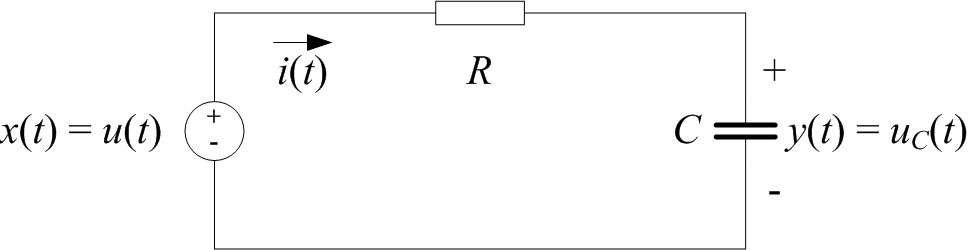
\includegraphics[height=2cm]{1.5.1-1.png}
\end{figure}

根据之前的分析,系统的微分方程模型:
\[
\frac{dy}{dt}+\frac{1}{RC}y=\frac{1}{RC}x \qquad \begin{cases}
	x\left( t \right) =u\left( t \right)\\
	y\left( 0^- \right) =0\\
\end{cases}
\]
求解该微分方程得到输出信号:
\begin{align*}
y\left( t \right) &=e^{-Pt}\left[ e^{Pt_0}y\left( t_0 \right) +Q\int_{t_0}^t{e^{P\tau}x\left( \tau \right) d\tau} \right] \\
&=e^{-\frac{1}{RC}t}\left[ y\left( 0 \right) +\frac{1}{RC}\int_0^t{e^{\frac{1}{RC}\tau}u\left( \tau \right) d\tau} \right] \\
&=\frac{1}{RC}e^{-\frac{1}{RC}t}\left[ \int_0^t{e^{\frac{1}{RC}\tau}d\tau} \right] =\frac{1}{RC}e^{-\frac{1}{RC}t}\left[ \left. RCe^{\frac{1}{RC}\tau} \right|_{0}^{t} \right] \\
&=1-e^{-\frac{t}{RC}} \qquad t\geqslant 0
\end{align*}
画图如下,可见,减小电阻或电容都可以提高输出对输入的“跟随性”。

\begin{python}
t  = np.arange(0, 10, 0.01)
RC = 1;   y1 = 1 - np.exp(-1 * t / RC)
RC = 0.1; y2 = 1 - np.exp(-1 * t / RC)

ax.plot(t, y1,       label='RC=1')
ax.plot(t, y2, '--', label='RC=0.1')
\end{python}

\begin{figure}[h]
\centering
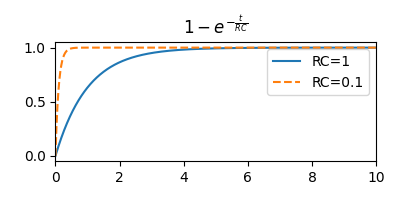
\includegraphics[height=3cm]{2.1.3-1.png}
\end{figure}






\newpage
\section{LTI系统的差分方程模型}

本节讨论离散系统的差分方程模型。

本节要点:
\begin{itemize}
    \item 掌握差分方程的概念;
    \item 理解差分方程的物理意义;
    \item 掌握差分方程的求解思路;
    \item 编写Python函数求解n阶线性常系数差分方程。
\end{itemize}

%============================================================
\subsection{差分方程的概念}

如果离散LTI系统有限维度,可以用线性常系数差分方程描述如下:
\[
y\left[ n \right] +\sum_{i=1}^N{A_iy\left[ n-i \right]}=\sum_{i=0}^M{B_ix\left[ n-i \right]}
\]
即系统某刻的输出$y\left[ n \right] $,由此刻的输入$x\left[ n \right] $和之前的输入$x\left[ n-i \right] $和之前的输出$y\left[ n-i \right] $,一共$N+M+1$个量共同决定。
通常配合初始条件,通过递归计算的方法就可以解出$y\left[ n \right] $。
这样的系统称为{\bf 递归型离散系统}(recursive discrete-time system)或{\bf 递归型数字滤波器}(recursive digital filter)。

%============================================================
\subsection{差分方程的物理意义}

以一阶差分方程为例:
\[
y\left[ n \right] +Ay\left[ n-1 \right] =Bx\left[ n \right]
\]
表示系统当刻输出$y\left[ n \right] $是当刻输入$x\left[ n \right] $和前刻输出$y\left[ n-1 \right] $的线性叠加。

这里要注意:
\begin{itemize}
    \item $B$:对系统稳定性来讲没有任何关系,只是表明系统是放大器还是衰减器;
    \item $y\left[ n-1 \right] $:表示系统内部对能量的回响;
    \item $A$:表示这种回响以反馈的方式造成混响,决定了系统的稳定性。
\end{itemize}
还要特别注意,这种回响不是一次性的,它造成的叠加输出在后一刻继续以混响的方式反馈于系统。
如果系统是LTI,则这种回响是关于时间的一个等比数列,造成的混响就是这个等比数列的和。

%============================================================
\subsection{一阶差分方程的求解}

对于一阶差分方程$y\left[ n \right] +Ay\left[ n-1 \right] =Bx\left[ n \right] $,可以通过不断递归求解,这里直接给出解:
\[
y\left[ n \right] =\left( -A \right) ^ny\left[ 0 \right] +\sum_{i=1}^n{\left( -A \right) ^{n-1}Bx\left[ i \right]} \qquad n=1,2,\cdots
\]

%============================================================
\subsection{Python应用——n阶差分方程的实现}

这里,我们编写一个Python函数(my\_diff)用以求解n阶差分方程:
\[
y\left[ n \right] +\sum_{i=1}^N{A_iy\left[ n-i \right]}=B_0x\left[ n \right] +\sum_{i=1}^M{B_ix\left[ n-i \right]}
\]

已知(同时也是函数的参数):
\begin{itemize}
    \item 系数(按照差分方程的系数排序):
    \[
    A_1,A_2,\cdots ,A_N,B_0,B_1,B_2,\cdots ,B_M
    \]
    \item 初始条件(按时间从最远点到最近点排序):
    \[
    y\left[ -N \right] ,\cdots ,y\left[ -1 \right] ,x\left[ -M \right] ,\cdots ,x\left[ -1 \right]
    \]
    \item 输入信号序列:
    \[
    x\left[ 1 \right] ,x\left[ 2 \right] ,\cdots ,x\left[ n \right]
    \]
\end{itemize}
取$y\left[ 1 \right] ,y\left[ 2 \right] $观察:
\begin{align*}
y\left[ 1 \right] =&A_1y\left[ -N \right] +A_2y\left[ -N+1 \right] \cdots A_{N-1}y\left[ -2 \right] +A_Ny\left[ -1 \right] + \\
&B_1x\left[ -M \right] +B_2x\left[ -M+1 \right] \cdots B_{M-1}x\left[ -2 \right] +B_Mx\left[ -1 \right] + \\
&Bx\left[ 1 \right] \\
y\left[ 2 \right] =&A_1y\left[ -N+1 \right] +A_2y\left[ -N+2 \right] \cdots A_{N-1}y\left[ -1 \right] +A_Ny\left[ 1 \right] + \\
&B_1x\left[ -M+1 \right] +B_2x\left[ -M+2 \right] \cdots B_{M-1}x\left[ -1 \right] +B_Mx\left[ 1 \right] + \\
&Bx\left[ 2 \right]
\end{align*}

设计参数:
\begin{itemize}
    \item An:$N$维向量,表示$A_1,A_2,\cdots ,A_N$;
    \item Yn:$N$维向量,表示输出信号的初始值$y\left[ -1 \right] ,y\left[ -2 \right] ,\cdots ,y\left[ -N \right] $;
    \item Bm:$M$维向量,表示$B_1,B_2,\cdots ,B_M$;
    \item Xm:$M$维向量,表示输入信号的初始值$x\left[ -1 \right] ,x\left[ -2 \right] ,\cdots ,x\left[ -M \right] $;
    \item b:标量,表示$B_0$;
    \item X:表示输入信号$x\left[ 1 \right] ,x\left[ 2 \right] ,\cdots ,x\left[ n \right] $。
\end{itemize}

过程注解:
\begin{enumerate}
    \item 将Yn和Xm翻转,以匹配An和Bm;
    \item 构造输出Y,和X一样长度,填充0;
    \item 计算每个Y[i],期间更新Yn和Xm;
    \item 返回Y。
\end{enumerate}

注意:
\begin{itemize}
    \item An和Yn的长度必须一致;
    \item Bm和Xm的长度必须一致;
    \item b是标量;
    \item 最终输出信号Y的长度由输入信号X决定。
\end{itemize}

\begin{python}
def my_diff(
        An:np.ndarray, Yn:np.ndarray,
        Bm:np.ndarray, Xm:np.ndarray,
        b:float,
        X:np.ndarray
        ) -> np.ndarray:

    Yn = np.flipud(Yn)
    Xm = np.flipud(Xm)
    Y  = np.zeros_like(X)

    for i in range(X.shape[0]):
        Y[i] = b*X[i] + np.dot(Bm, Xm) - np.dot(An, Yn)
        Yn = np.append(Yn, Y[i])[1:]
        Xm = np.append(Xm, X[i])[1:]
        pass

    return Y
\end{python}






\newpage
\section{微分方程的离散化}

对于不容易求解的微分方程,比如高阶方程,可以通过对时间的离散化变成差分方程,再通过递归获得数值解。

本节要点:
\begin{itemize}
    \item 掌握欧拉近似方法。
\end{itemize}

%============================================================
\subsection{一阶微分方程的欧拉近似}

一阶常系数微分方程:
\[
\frac{dy}{dt}+Py=Qx \qquad t\geqslant t_0
\]
假设时间取离散点$t=nT$,则:
\[
\frac{dy\left( nT \right)}{d\left( nT \right)}+Py\left( nT \right) =Qx\left( nT \right) \qquad n=0,1,2,\cdots
\]
如果采样周期足够小,方程左边可以认为$\frac{1}{T}\left[ y\left( nT+T \right) -y\left( nT \right) \right] +Py\left( nT \right) $,于是一阶微分方程可以离散地表示为:
\[
y\left[ n \right] +\left( PT-1 \right) y\left[ n-1 \right] =TQx\left[ n-1 \right] \qquad n=0,1,2,\cdots
\]
该一阶差分方程即为一阶微分方程的近似,根据之前讨论的方法即可得到采样点的输出信号,该过程称为{\bf 欧拉近似}(Euler approximation)。
欧拉近似是一种对微分方程数值化求解的方法,采样周期越小,精度越高。

%============================================================
\subsection{二阶微分方程的欧拉近似}

对于二阶微分方程:
\[
\frac{d^2y}{dt^2}+A_1\frac{dy}{dt}+A_0y=B_1\frac{dx}{dt}+B_0x \qquad t\geqslant t_0
\]
用欧拉近似可得差分方程:
\begin{align*}
&\frac{y\left[ n \right] +y\left[ n-2 \right]}{T^2}+A_1\frac{y\left[ n-1 \right] -y\left[ n-2 \right]}{T}+A_0y\left[ n-2 \right] \\
&=B_1\frac{x\left[ n-1 \right] -x\left[ n-2 \right]}{T}+B_0x\left[ n-2 \right]
\end{align*}
整理后:
\begin{align*}
&y\left[ n \right] +\left( A_1T-2 \right) y\left[ n-1 \right] +\left( A_0T^2-A_1T+1 \right) y\left[ n-2 \right] \\
&=B_1Tx\left[ n-1 \right] +\left( B_0T^2-B_1T \right) x\left[ n-2 \right]
\end{align*}

%============================================================
\subsection{例RC电路}

\begin{example}
以下图为例,假设电路零状态,$x\left( t \right) =1\mathrm{V},R=1\Omega ,C=1\mathrm{F}$,分别用微分方程和差分方程计算系统在0~10s这段时间内的输出。
\end{example}

\begin{figure}[h]
\centering
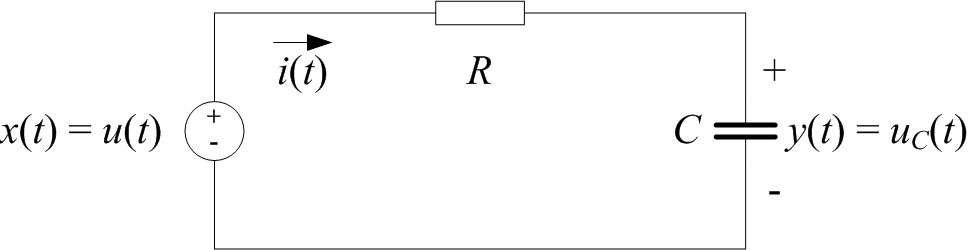
\includegraphics[height=2cm]{1.5.1-1.png}
\end{figure}
\[
\frac{dy}{dt}+\frac{1}{RC}y=\frac{1}{RC}x \qquad \begin{cases}
	x\left( t \right) =u\left( t \right)\\
	y\left( 0^- \right) =0\\
\end{cases}
\]

将之前的结果解得到输出信号并将其做欧拉近似得到差分方程:
\begin{align*}
&y\left( t \right) =1-e^{-\frac{t}{RC}}=1-e^{-t} \qquad t\geqslant 0 \\
&y\left[ n \right] +\left( T-1 \right) y\left[ n-1 \right] =Tx\left[ n-1 \right] \qquad n=0,1,2,\cdots
\end{align*}
令采样间隔$T=0.2\mathrm{s}$,微分方程和差分方程结果如下。

\begin{python}
T  = 0.2
An = np.array([T-1])
Bm = np.array([T])
b  = 0
Yn = np.array([0])
Xm = np.array([0])
t  = np.arange(0, 10, T)
X  = np.ones_like(t)
Y_differential = 1 - np.exp(-1*t)
Y_difference   = my_diff(An, Yn, Bm, Xm, b, X)

ax.plot(t, Y_differential,      label='differential')
ax.plot(t, Y_difference,   'o', label='difference')
\end{python}

\begin{figure}[h]
\centering
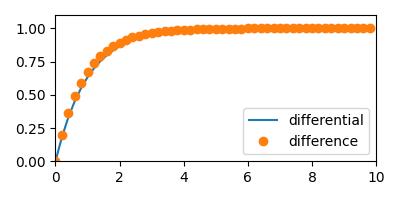
\includegraphics[height=3cm]{2.3.3-1.png}
\end{figure}






\newpage
\section{本章小结}

本章介绍了有限维度LTI系统的两种模型,微分方程模型和差分方程模型。

微分方程模型是最基本、最直观的物理模型。
由于本书只从信号与系统的角度阐述微分方程,所以建议与微积分中的微分方程章节,和选一门工科基础课程(如电路原理)中的微分方程章节,一起相互印证学习。

差分方程模型是微分方程模型的数值化计算,主要掌握离散化方法即可。










\chapter{卷积}

卷积本身是一种计算方法,从数学上来说是一种加权和。

系统在时域可以用另一种方法描述——冲激响应,即对冲激信号的响应。
当系统用冲激响应描述时,输出就是输入和冲激响应的卷积,这就是系统的卷积模型。

冲激响应可以通过求解微分或差分方程得到,前者得到解析解,后者得到一系列数值。
但更多情况下,通过实验测得,所以如何获得冲激响应不是本章所要讨论的。

本章重点在于介绍连续信号和离散信号的卷积。
由于离散信号的卷积更能说明计算过程,所以先介绍离散信号的卷积。

本章要点:
\begin{itemize}
    \item 离散LTI系统的卷积模型。
    \item 连续LTI系统的卷积模型。
    \item 卷积的运算法则。
\end{itemize}

\newpage
\section{离散LTI系统的卷积模型}

本节介绍离散LTI系统在时域的卷积模型。

本节要点:
\begin{itemize}
    \item 了解卷积和的概念;
    \item 熟悉卷积和的物理意义;
    \item 熟悉Numpy的卷积函数。
\end{itemize}

%============================================================
\subsection{卷积的导出过程}

\begin{definition}[冲激响应]
我们称单位冲激信号$\delta \left[ n \right] $经过零状态系统后的输出为{\bf 单位冲激响应},简称{\bf 冲激响应}(pulse response),记为$h\left[ n \right] $。
\end{definition}

继续以RC电路为例,取采样间隔0.2s,差分方程:
\[
y\left[ n \right] =0.8y\left[ n-1 \right] +0.2x\left[ n-1 \right] \qquad n=0,1,2,\cdots
\]
对于冲激输入,我们可以通过之前的方法获得其响应,如下左图。
由于系统的LTI性,对于等比例冲激输入和时移的冲激输入,都有同样的等比输出和时移输出。
假设时移并放大至$3\delta \left[ n-4 \right] $,响应如下右图。
\begin{figure}[h]
\centering
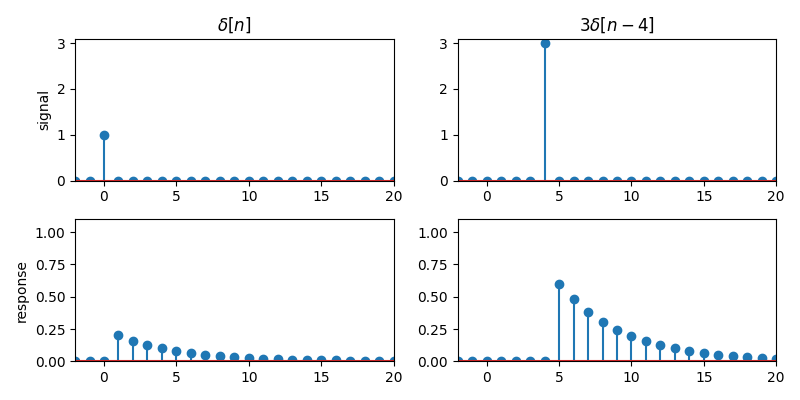
\includegraphics[height=5cm]{3.1.1-1.png}
\end{figure}

由于输入信号可以视为一系列冲激的和,相应地,输出信号也可以视为一系列冲激响应的和:
\begin{align*}
&x\left[ n \right] =\sum_{i=0}^{\infty}{x\left[ i \right] \delta \left[ n-i \right]} \qquad n=0,1,2,\cdots \\
&y\left[ n \right] =\sum_{i=0}^{\infty}{x\left[ i \right] h\left[ n-i \right]} \qquad n=0,1,2,\cdots
\end{align*}

举例说明,假设输入信号$x\left[ n \right] $和系统的冲激响应$h\left[ n \right] $如下:
\begin{figure}[ht]
\centering
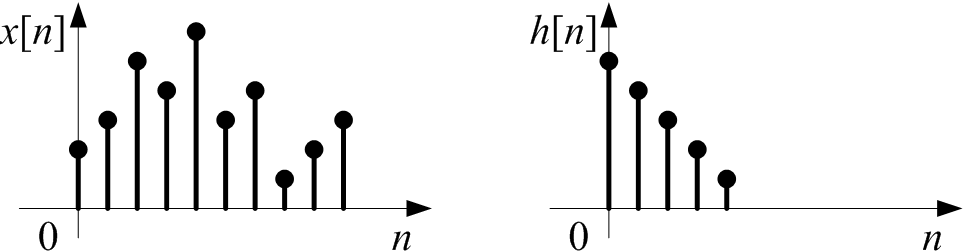
\includegraphics[height=2cm]{3.1.1-3.png}
\end{figure}

若要获得输出$y\left[ 3 \right] $,则系统会对输入$x\left[ 0 \right] ,x\left[ 1 \right] ,x\left[ 2 \right] ,x\left[ 3 \right] $进行“加权叠加响应”,如下左图。
如果要获得输出$y\left[ 9 \right] $,由于系统的响应只到$h\left[ 4 \right] $,所以系统只对$x\left[ 5 \right] ,x\left[ 6 \right] ,x\left[ 7 \right] ,x\left[ 8 \right] ,x\left[ 9 \right] $进行“加权叠加响应”,如下右图。
\begin{figure}[h]
\centering
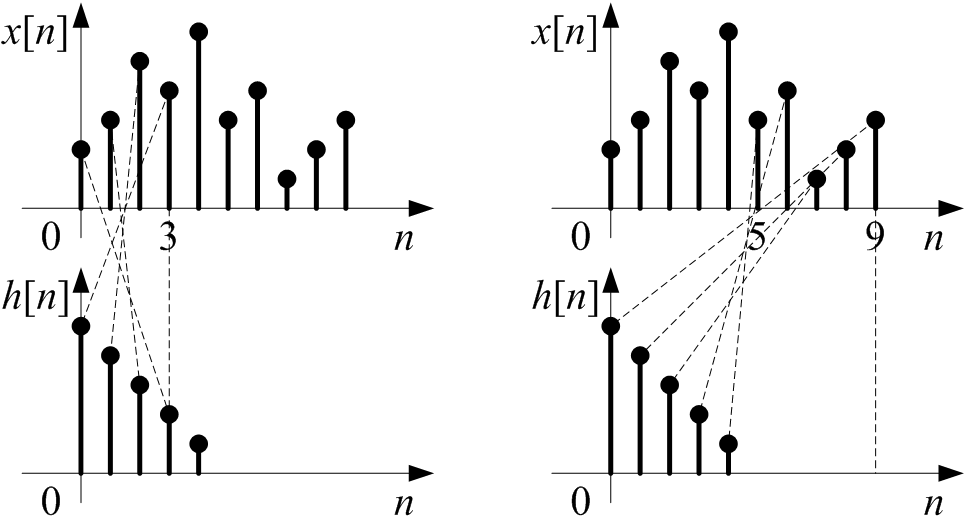
\includegraphics[height=4cm]{3.1.1-4.png}
\end{figure}

从数学角度看,$n$刻的输出$y\left[ n \right] $是$n$刻及之前时刻的输入$x\left[ i \right] ,i=0,1,2,\cdots ,n$的加权和,对应的权重为$h\left[ n-i \right] ,i=0,1,2,\cdots ,n$,可以理解“翻转+时移”。
\begin{figure}[h]
\centering
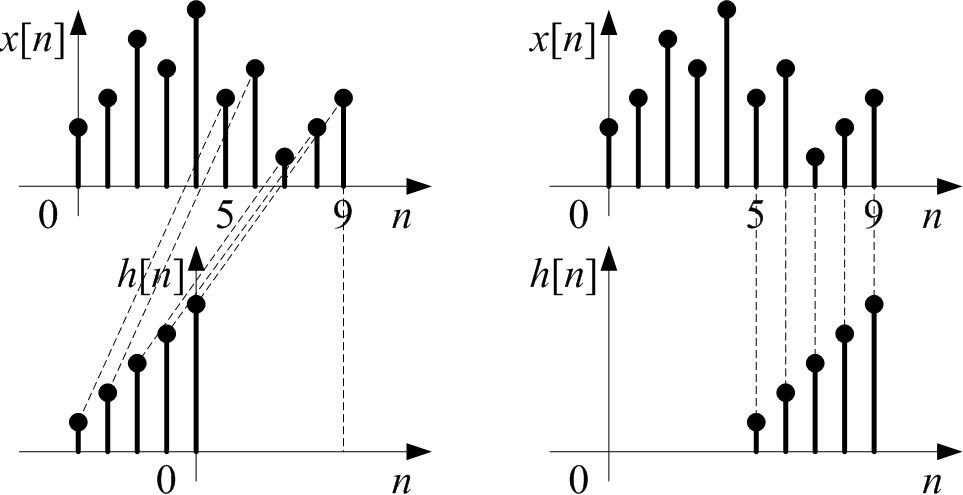
\includegraphics[height=4cm]{3.1.1-5.png}
\end{figure}
\[
y\left[ n \right] =\left[ \begin{matrix}
	x\left[ 0 \right]&		x\left[ 1 \right]&		\cdots&		x\left[ n-1 \right]&		x\left[ n \right]\\
\end{matrix} \right] \cdot \left[ \begin{array}{c}
	h\left[ n \right]\\
	h\left[ n-1 \right]\\
	\vdots\\
	h\left[ 1 \right]\\
	n\left[ 0 \right]\\
\end{array} \right]
\]

%============================================================
\subsection{卷积和和卷积模型}

\begin{definition}[卷积和]
对于两个离散函数$a\left[ n \right] ,b\left[ n \right] ,n\in \mathbb{Z} $,如果和式$\sum_{i=-\infty}^{+\infty}{a\left[ i \right] b\left[ n-i \right]}$收敛,则称其为{\bf $a\left[ n \right] ,b\left[ n \right] $的卷积和}(convolution sum),记为$a\left[ n \right] \ast b\left[ n \right] $,即:
\[
a\left[ n \right] \ast b\left[ n \right] =\sum_{i=-\infty}^{+\infty}{a\left[ i \right] b\left[ n-i \right]}
\]
\end{definition}

可见,卷积和是“一个和,一个加权和,一个反置移位的加权和”。

~

{\bf 离散LTI系统的卷积模型}:设一离散LTI系统符合因果律且零状态,若对单位冲激信号$\delta \left[ n \right] $的响应$h\left[ n \right] $已知,则该系统对任何输入信号的响应可以表示为输入信号$x\left[ n \right] $和冲激响应$h\left[ n \right] $的卷积,即:
\[
y\left[ n \right] =x\left[ n \right] \ast h\left[ n \right] =\begin{cases}
	0 &n=-1,-2,\cdots\\
	\sum_{i=0}^n{x\left[ i \right] h\left[ n-i \right]} &n=0,1,2,\cdots\\
\end{cases}
\]
该表达式称为{\bf 系统的卷积模型}。

从混响和回响的角度,输出$y\left[ n \right] $可以理解为一系列输入产生的系统回响$x\left[ i \right] h\left[ n-i \right] $的叠加。
只是要特别注意,$i$刻的回响不是$x\left[ i \right] h\left[ i \right] $,而是$x\left[ i \right] h\left[ n-i \right] $。
如0刻的回响是$x\left[ 0 \right] h\left[ n \right] $,因为此时回响已经经历了时间$n$,$n$刻的回响是$x\left[ n \right] h\left[ 0 \right] $。

%============================================================
\subsection{差分方程模型和卷积模型}

至此,对于一个LTI系统,我们可以用差分方程和卷积两种方法描述:
\begin{align*}
&y\left[ n \right] +\sum_{i=1}^N{A_iy\left[ n-i \right]}=\sum_{i=0}^M{B_ix\left[ n-i \right]} \\
&y\left[ n \right] =x\left[ n \right] \ast h\left[ n \right]
\end{align*}
两种模型都要求系统是LTI,区别在于:
\begin{itemize}
    \item 差分方程要求是有限维度,用系数$A_1\cdots A_N,B_0,B_1,\cdots ,B_M$描述系统,不同系统的区别就在于不同的系数。
    \item 卷积要求符合因果律,用冲激响应$h\left[ n \right] $描述系统,不同系统的区别在于不同的$h\left[ n \right] $。
\end{itemize}

%============================================================
\subsection{卷积的物理意义}

结合记忆和因果,卷积的物理意义就很明显。
由于系统的内部构造,系统对输入的能量会有惯性,冲激能量$\delta \left[ n \right] $在内部会造成一个回响$h\left[ n \right] $。
只要系统是LTI,输出$y \left[ t \right]$就是此刻及之前每刻的回响的混响$\sum_{i=0}^n{x\left[ i \right] h\left[ n-i \right]}$。
回响是惯性的表现,混响是LTI的结果,所以卷积是LTI的必然结果。
若将系统分为几个子系统,由于LTI的关系,系统的最终表现与子系统在空间上的组合和时间上的前后无关,数学上表示为卷积的分配率和结合律。

%============================================================
\subsection{Python应用——numpy.convolve()函数}

numpy提供了卷积函数convolve()。
\begin{figure}[h]
\centering
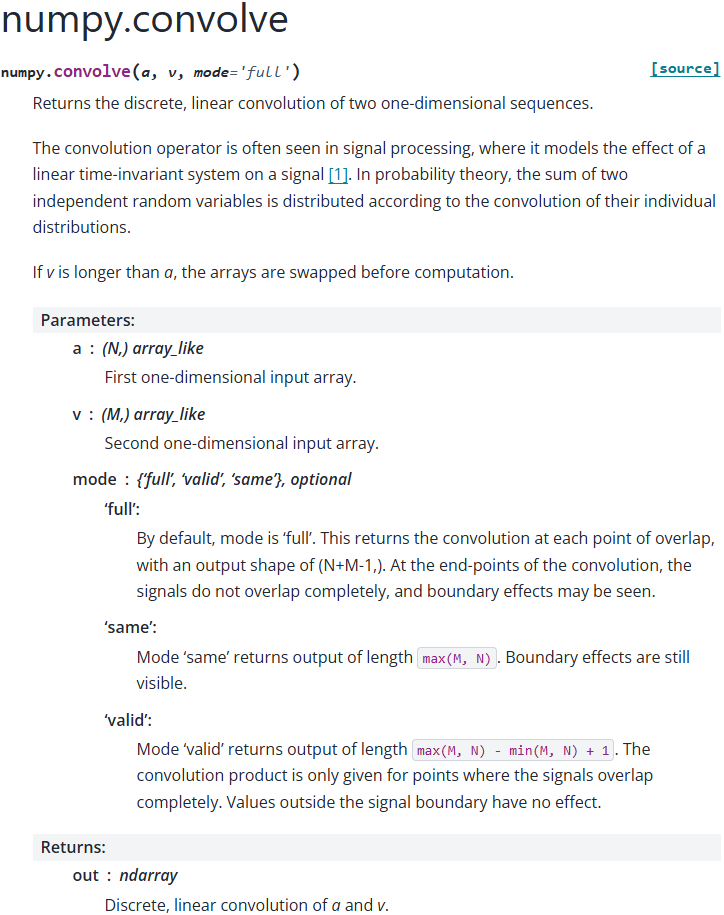
\includegraphics[width=10cm]{3.1.5-1.png}
\end{figure}

假设系统的差分方程为:
\[
y\left[ n \right] -0.8y\left[ n-1 \right] =0.2x\left[ n-1 \right]
\]
通过my\_diff函数可以获得冲激响应,取前11个值:
\begin{center}
h = [0, 0.2, 0.16, 0.128, 0.1024, 0.0819, 0.0655, 0.0524, 0.0419, 0.0336, 0.0268]
\end{center}
用np.convolve()计算冲激响应和输入信号(单位阶跃)的卷积,对比差分方程的计算:

\begin{python}
An = np.array([-0.8]); Bm = np.array([0.2]); b = 0
Yn = np.array([0]);    Xm = np.array([0])

n  = np.arange(-2, 21, 1)
X  = np.zeros_like(n, dtype=np.float64)
X[2:] = 1.0
Yd = my_diff(An, Yn, Bm, Xm, b, X)
h  = np.array([0.0, 0.2, 0.16, 0.128, 0.1024, 0.0819, 0.0655, 0.0524, 0.0419, 0.0336, 0.0268])
Yc = np.convolve(X, h, mode='full')
\end{python}

\begin{itemize}
    \item Yd是我们my\_diff()函数的计算结果;
    \item Yc是用Numpy的convolve()函数的计算结果,注意它认为输入是方波,所以长度会比较长,绘制Yc时需要截断;
    \item 由于我们的h只取了前11个,所以计算得到的值并没有“长足”。
\end{itemize}

\begin{figure}[h]
\centering
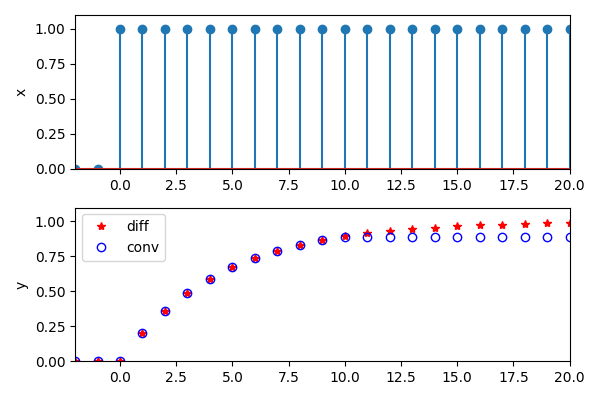
\includegraphics[height=5cm]{3.1.5-2.png}
\end{figure}






\newpage
\section{连续LTI系统的卷积模型}

本节讨论LTI系统在连续时域的卷积模型。

本节要点:
\begin{itemize}
    \item 理解卷积积分的概念;
    \item 掌握LTI系统的卷积模型;
    \item 熟悉卷积模型对系统的要求。
\end{itemize}

%============================================================
\subsection{卷积积分和卷积模型}

\begin{definition}[冲激响应]
我们称单位冲激信号$\delta \left( t \right) $经过系统后的输出称为{\bf 单位冲激响应},简称{\bf 冲激响应},记为$h\left( t \right) $。
\end{definition}

\begin{definition}[卷积积分]
对于两个连续函数$a\left( t \right) ,b\left( t \right) ,t\in \mathbb{R} $,如果广义积分$\int_{-\infty}^{+\infty}{a\left( \tau \right) b\left( t-\tau \right) d\tau}$收敛,则称该积分为{\bf $a\left( t \right) ,b\left( t \right) $的卷积积分}(convolution integral),记为$a\left( t \right) \ast b\left( t \right) $,即:
\[
a\left( t \right) \ast b\left( t \right) =\int_{-\infty}^{+\infty}{a\left( \tau \right) b\left( t-\tau \right) d\tau}
\]
\end{definition}

{\bf 连续LTI系统的卷积模型}:若一LTI系统符合因果律且零状态,系统的冲激响应为$h\left( t \right) $,当$h\left( t \right) $和输入信号$x\left( t \right) $在$\left[ 0,t \right] $绝对可积:
\begin{align*}
&\int_0^t{\left| x\left( \tau \right) \right|d\tau}<\infty \\
&\int_0^t{\left| h\left( \tau \right) \right|d\tau}<\infty
\end{align*}
则该系统对任何输入信号的响应可以表示为输入信号$x\left( t \right) $和冲激响应$h\left( t \right) $的卷积,即:
\[
y\left( t \right) =x\left( t \right) \ast h\left( t \right) =\begin{cases}
	0 &t<0\\
	\int_0^t{x\left( \tau \right) h\left( t-\tau \right) d\tau} &t\geqslant 0\\
\end{cases}
\]
该表达式称为{\bf 系统的卷积模型}。

%============================================================
\subsection{微分方程模型和卷积模型}

至此,对于一个LTI系统,我么可以用微分方程和卷积两种方法描述:
\begin{align*}
&y^{\left( n \right)}\left( t \right) +\sum_{i=0}^{n-1}{A_iy^{\left( i \right)}\left( t \right)}=\sum_{i=0}^m{B_ix^{\left( i \right)}\left( t \right)} \\
&y\left( t \right) =x\left( t \right) \ast h\left( t \right)
\end{align*}
两种模型都要求系统是LTI,区别在于:
\begin{itemize}
    \item 微分方程要求是有限维度,用系数$A_0,A_1,\cdots ,A_{n-1},B_0,B_1,\cdots ,B_m$描述系统,不同系统的区别就在于不同的系数。
    \item 卷积要求是符合因果律,再加上$x\left( t \right) ,h\left( t \right) $绝对可积,用冲激响应$h\left( t \right) $描述系统,不同系统的区别在于不同的$h\left( t \right) $。
\end{itemize}
两个模型中,微分方程对应着卷积运算,微分方程的系数对应着冲激响应。

%============================================================
\subsection{一阶微分方程系统的零状态冲激响应}

对于一阶微分方程的系统$\frac{dy\left( t \right)}{dt}+Py\left( t \right) =Qx\left( t \right) $,考虑零状态($y\left( 0 \right) =0$)响应:
\[
y\left( t \right) =e^{-Pt}\left[ e^{-Pt_0}y\left( t_0 \right) +Q\int_{t_0}^t{e^{-P\tau}x\left( \tau \right) d\tau} \right] =e^{-Pt}\left[ Q\int_0^t{e^{-P\tau}x\left( \tau \right) d\tau} \right]
\]
冲激响应:
\[
h\left( t \right) =\left. y \right|_{x=\delta}=e^{-Pt}\left[ Q\int_0^t{e^{-P\tau}\delta \left( \tau \right) d\tau} \right] =Qe^{-Pt}
\]
可见,零状态的一阶微分系统有着一样的冲激响应。

%============================================================
\subsection{例RC电路}

\begin{example}
依然以RC电路为例,(1)试从微分方程推导系统的冲激响应,(2)写出系统的卷积模型,(3)如果输入信号为$x\left( t \right) =1$,求解输出。
\end{example}
\begin{figure}[h]
\centering
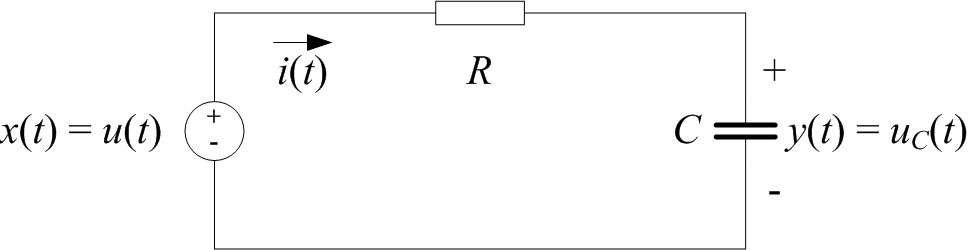
\includegraphics[height=2cm]{1.5.1-1.png}
\end{figure}


(1)令输入信号为冲激函数,求解得到冲激响应:
\begin{align*}
&\because \frac{dy}{dt}+\frac{1}{RC}y=\frac{1}{RC}x \qquad \begin{cases}
	x\left( t \right) =\delta \left( t \right)\\
	y\left( 0^- \right) =0\\
\end{cases} \\
&\therefore h\left( t \right) =e^{-Pt}\left[ Q\int_0^t{e^{-P\tau}\delta \left( \tau \right) d\tau} \right] =\frac{1}{RC}e^{-\frac{t}{RC}}
\end{align*}

(2)系统的卷积模型:
\[
y\left( t \right) =x\left( t \right) \ast h\left( t \right) =\int_0^t{x\left( \tau \right) \frac{1}{RC}e^{-\frac{t-\tau}{RC}}d\tau} \qquad t\geqslant 0
\]

(3)将输入信号带入,计算得到输出:
\[
y\left( t \right) =\int_0^t{\frac{1}{RC}e^{-\frac{t-\tau}{RC}}d\tau}=1-e^{-\frac{t}{RC}} \qquad t\geqslant 0
\]






\newpage
\section{卷积的运算法则}

本节特别把离散卷积和连续卷积的运算法则放在一起,方便查询。

~

{\bf 交换律}
\begin{align*}
&a\left( t \right) \ast b\left( t \right) =b\left( t \right) \ast a\left( t \right) \\
&a\left[ n \right] \ast b\left[ n \right] =b\left[ n \right] \ast a\left[ n \right]
\end{align*}

{\bf 结合律}
\begin{align*}
&\left( a\left( t \right) \ast b\left( t \right) \right) \ast c\left( t \right) =a\left( t \right) \ast \left( b\left( t \right) \ast c\left( t \right) \right) \\
&\left( a\left[ n \right] \ast b\left[ n \right] \right) \ast c\left[ n \right] =a\left[ n \right] \ast \left( b\left[ n \right] \ast c\left[ n \right] \right)
\end{align*}

{\bf 分配律}
\begin{align*}
&a\left( t \right) \ast \left( b\left( t \right) +c\left( t \right) \right) =a\left( t \right) \ast b\left( t \right) +a\left( t \right) \ast c\left( t \right) \\
&a\left[ n \right] \ast \left( b\left[ n \right] +c\left[ n \right] \right) =a\left[ n \right] \ast b\left[ n \right] +a\left[ n \right] \ast c\left[ n \right]
\end{align*}

{\bf 时移律}
\begin{align*}
&a\left( t-c \right) \ast b\left( t \right) =a\left( t \right) \ast b\left( t-c \right) \\
&a\left[ n-i \right] \ast b\left[ n \right] =a\left[ n \right] \ast b\left[ n-i \right]
\end{align*}

{\bf 冲激的卷积}(冲激卷积会造成时移,相当于一个延时器)
\begin{align*}
&a\left( t \right) \ast \delta \left( t-c \right) =a\left( t-c \right) \\
&a\left[ n \right] \ast \delta \left[ n-i \right] =a\left[ n-i \right]
\end{align*}

{\bf 阶跃的卷积}(阶跃卷积是作积分,相当于通过一个积分器)
\[
a\left( t \right) \ast u\left( t \right) =\int_{-\infty}^t{a\left( \tau \right) d\tau}
\]

{\bf 导数律}
\begin{align*}
&\frac{d}{dt}\left[ a\left( t \right) \ast b\left( t \right) \right] =a'\left( t \right) \ast b\left( t \right) =a\left( t \right) \ast b'\left( t \right) \\
&\frac{d^2}{dt^2}\left[ a\left( t \right) \ast b\left( t \right) \right] =a'\left( t \right) \ast b'\left( t \right)
\end{align*}

{\bf 积分律}
\[
\int_{-\infty}^t{\left[ a\left( \tau \right) \ast b\left( \tau \right) \right] d\tau}=\left[ \int_{-\infty}^t{a\left( \tau \right) d\tau} \right] \ast b\left( t \right) =a\left( t \right) \ast \left[ \int_{-\infty}^t{b\left( \tau \right) d\tau} \right]
\]






\newpage
\section{本章小结}

至此,时域上的分析方法都已介绍完毕。
系统在时域本质上就是回响的混响,所以时域模型就是研究回响和混响。

\begin{figure}[h]
\centering
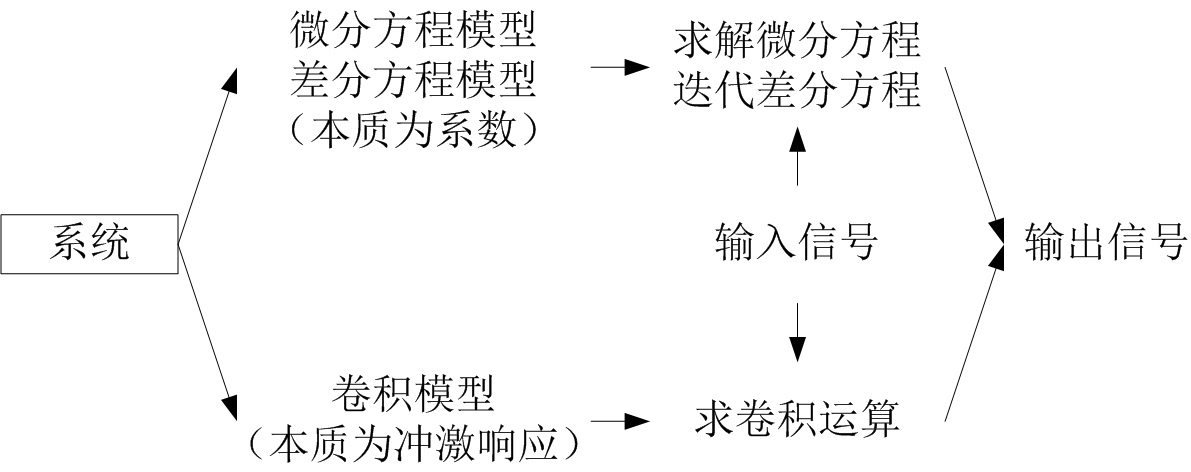
\includegraphics[height=4cm]{3.4-1.png}
\end{figure}

时域分析的目的是在已知输入的情况下求解系统的输出。
为此,需要两个步骤:1)建立系统模型,2)对于给定输入计算输出。

系统的两种时域模型:
\begin{itemize}
    \item 微分/差分方程:系数表示系统回响,微分方程表示系统混响,难在求解微分方程;
    \item 卷积:冲激响应表示回响,卷积运算表示混响,难在获得系统的冲激响应,注意冲激响应描述的是系统对冲激函数的响应,而非输入输出关系。
\end{itemize}

有了模型之后,求解输出:
\begin{itemize}
    \item 微分/差分方程:将输入信号带入方程求解输出的解析解,或用迭代法求解输出信号的数值序列;
    \item 卷积:将输入信号和冲激响应作卷积运算,获得输出信号。
\end{itemize}










\chapter{傅里叶变换}

本章起至第六章介绍傅里叶变换。
傅里叶变换是对信号的处理,不描述系统,但它是后续讨论系统传递函数和其他各种变换的基础。

本章从三角级数和傅里叶级数入手,引出傅里叶变换。
信号与系统中的傅里叶变换着重性质和应用,不太重视来源和推导过程,这部分是在微积分中讲授,所以学习本章最好配合微积分教材中的级数章节,特别是三角级数、傅里叶级数和傅里叶积分,相互印证着看。
本章最后给出Python应用,介绍如何使用Python求解傅里叶变换和逆变换。

本章要点:
\begin{itemize}
    \item 傅里叶变换。
\end{itemize}

~

本章至第六章的结构:
\begin{itemize}
    \item {\bf 第四章 \, 傅里叶变换}:介绍连续时域的傅里叶变换(CTFT),系统地讲述傅里叶变换的概念和性质,是后续两章的基础;
    \item {\bf 第五章 \, 系统的频率分析}:从频率角度考察系统,算作是CTFT的一个简单应用;
    \item {\bf 第六章 \, 离散傅里叶变换}:介绍离散傅里叶变换(DFT),由于现代数字处理芯片的使用,所以DFT是学习整个傅里叶变换的目标。
\end{itemize}

\newpage
\section{周期信号的傅里叶级数型}

本节简单介绍周期信号的傅里叶级数,具体推导参见《微积分笔记》。

本节要点:
\begin{itemize}
    \item 掌握傅里叶级数的三角级数形式;
    \item 掌握傅里叶级数的复指数形式;
    \item 理解傅里叶级数的量纲;
    \item 熟练掌握周期信号的复指数展开。
\end{itemize}

%============================================================
\subsection{三角级数展开}

{\bf 三角级数展开}:当周期为$T$的信号$x\left( t \right) $满足狄利克雷收敛条件时,其在周期内可以展开成三角级数,即无穷项余弦函数的叠加,且收敛于该周期信号:
\[
x\left( t \right) =A_0+\sum_{n=1}^{+\infty}{A_n\cos \left( \omega _nt+\varphi _n \right)}
\]
\begin{itemize}
    \item $A_0,A_n$:{\bf 傅里叶系数},$A_0$表示信号的{\bf 直流分量}或{\bf 基频分量};
    \item $\omega _n=n\omega _0$:对应余弦项的{\bf 角频},称$\omega _0=2\pi /T$为{\bf 基频};
    \item $\varphi _n$:对应余弦项的{\bf 初始相位},简称{\bf 相位}。
\end{itemize}

数学上,周期函数都能展开成三角级数,但不一定收敛,即便收敛也不一定收敛至原函数。
如果周期函数满足狄利克雷充分条件,即周期函数必须在一个包含原点的最小周期内连续,或只有有限个一类间断点,而且只有有限个极值点,则三角级数收敛在原函数。
这样的三角级数称为傅里叶级数。

周期信号展开成三角级数后,对信号又多了一种描述方法,即以频率$\omega _n$为自变量,幅值和初相为因变量的两个函数$A\left( \omega _n \right) ,\varphi \left( \omega _n \right) $:
\[
x=x\left( t \right) ,T=\frac{2\pi}{\omega _0} \quad \Leftrightarrow \quad \begin{cases}
	A=A\left( \omega _n \right)\\
	\varphi =\varphi \left( \omega _n \right)\\
\end{cases}
\]
在图形方面,原本只有时域上的波形图,现在多了两张频域上的图形,称为{\bf 幅频图}(amplitude spectrum) 和{\bf 相频图}(phase spectrum) ,统称为{\bf 频谱图}。

%============================================================
\subsection{复指数级数展开}

{\bf 复指数级数展开}:当周期为$T$的信号$x\left( t \right) $满足狄利克雷收敛条件时,其在周期内可以展开成复指数级数形式,且收敛于该周期信号:
\begin{align*}
&x\left( t \right) =C_0+\sum_{n=-\infty ,n\ne 0}^{+\infty}{\left( C_ne^{i\omega _nt} \right)} \\
&\begin{cases}
	C_0=\frac{1}{T}\int_{-\frac{T}{2}}^{\frac{T}{2}}{x\left( t \right) dt}\\
	C_n=\frac{1}{T}\int_{-\frac{T}{2}}^{\frac{T}{2}}{x\left( t \right) e^{-i\omega _nt}dt}\\
\end{cases}
\end{align*}
\begin{itemize}
    \item $C_0,C_n$:{\bf 傅里叶系数的复数形式};
    \item $\omega _n=n\omega _0$:对应{\bf 复指数项的角频},$\omega _0=2\pi /T$称为{\bf 基频}。
\end{itemize}
该级数称为{\bf 傅里叶级数的复数形式}。
此时的信号可以用以频率$\omega _n$为自变量的复函数$C=C\left( \omega _n \right) $表示:
\[
x=x\left( t \right) ,T=\frac{2\pi}{\omega _0} \quad \Leftrightarrow \quad C=C\left( \omega _n \right)
\]

由欧拉公式可得三角级数和复指数级数的关系:
\begin{align*}
&x\left( t \right) =A_0+\sum_{n=1}^{+\infty}{A_n\cos \left( \omega _nt+\varphi _n \right)}=C_0+\sum_{n=-\infty ,n\ne 0}^{+\infty}{\left( C_ne^{i\omega _nt} \right)} \\
&\begin{cases}
	A_0=C_0\\
	A_n=2\left| C_n \right|\\
	\varphi _n=\angle C_n\\
\end{cases}
\end{align*}
且常称$A_n\cos \left( \omega _nt+\varphi _n \right) $为{\bf {\it n}次谐波}({\it n}th harmonic)。

由于信号是周期性,所以频率虽然是无穷多,但还是取离散的值$n\omega _0$。复指数形式中,首先将相位和振幅合并成一个复数;其次,通过引入“负频率”制造一对共轭对,一起表示该频率的{\it n}次谐波分量$C_ne^{i\omega _nt}+C_{-n}e^{i\omega _{-n}t}=A_n\cos \left( n\omega _0t+\varphi _n \right) $。
最后需要注意的是,不同的周期信号,在时域上表现为不同的波形$x\left( t \right) $,在频域上则表现为不同的傅里叶系数$C_n$,所以频域的频谱图是和时域的波形图一样真实的存在。

\begin{theorem}[Parseval定理]
周期信号的功率为$P=\frac{1}{T}\int_{-\frac{T}{2}}^{\frac{T}{2}}{\left| x\left( t \right) \right|^2dt}$,若信号展开成傅里叶级数,功率可以表示为:
\[
P=\sum_{n=-\infty}^{+\infty}{\left| C_n \right|^2}
\]
\end{theorem}

%============================================================
\subsection{傅里叶级数的量纲}

物理上,只有具有相同量纲的变量才可以作加减,所以$x\left( t \right) ,A_0,A_n$具有相同的量纲,$\omega _n$的量纲是$\mathrm{rad}\cdot \mathrm{s}^{-1}$,$\varphi _n$的量纲是$\mathrm{rad}$。对于复指数级数,通过引入负频率,我们用一对共轭复数$C_ne^{i\omega _nt},C_{-n}e^{i\omega _{-n}t}$对表示信号在某个频率的成分,即:
\[
C_ne^{i\omega _nt}+C_{-n}e^{i\omega _{-n}t}=2\left| C_n \right|\cos \left( \omega _nt+\angle C_n \right) =A_n\cos \left( \omega _nt+\varphi _n \right)
\]
所以,$x\left( t \right) ,C_n$具有相同量纲。

虽然$x\left( t \right) ,C_n$具有相同量纲,但因为它们总是以共轭对的形式出现,所以单独$C_n$讨论没有意义,只需要考察正频率部分即可。

\begin{tcolorbox}
量纲的概念需要贯穿始终。
\end{tcolorbox}

%============================================================
\subsection{复指数级数展开的步骤}

周期信号展开成傅里叶级数(这里指复指数形式)时,只要级数项的个数足够多就能足够描述原信号。

展开步骤为:
\begin{enumerate}
    \item 根据信号周期$T$确定基频及各个谐波频率:
    \[
    \omega _0=\frac{2\pi}{T} \qquad \omega _n=n\omega _0=\frac{2n\pi}{T}
    \]
    \item 计算直流分量和谐波的傅里叶系数:
    \[
    C_0=\frac{1}{T}\int_{-\frac{T}{2}}^{\frac{T}{2}}{x\left( t \right) dt} \qquad C_n=\frac{1}{T}\int_{-\frac{T}{2}}^{\frac{T}{2}}{x\left( t \right) e^{-i\omega _nt}dt}
    \]
    \item 计算得到信号的展开式:
    \[
    x\left( t \right) =C_0+\sum_{n=\pm 1}^{\pm \infty}{\left( C_ne^{i\omega _nt} \right)}
    \]
\end{enumerate}

通过对量纲的分析可知,即便采用复指数形式展开,依然必定是不含虚数的!
也就是说,$C_n$可以有虚部,但$x\left( t \right) $的展开结果必然是通过$\pm n$抵消虚部。

%============================================================
\subsection{例}

~

\begin{example}
假设如下图方波,求其傅里叶级数,并用Python画图验证。
\begin{figure}[ht]
\centering
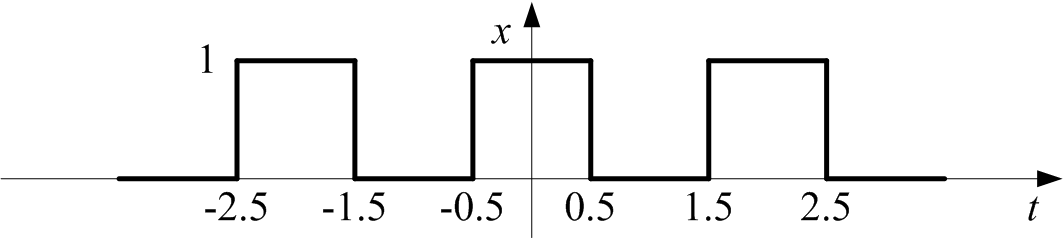
\includegraphics[height=2cm]{4.1.5-1.png}
\end{figure}
\end{example}

易得$T=2,\omega _0=\pi ,\omega _n=n\pi $,计算傅里叶系数:
\begin{align*}
C_0&=\frac{1}{T}\int_{-\frac{T}{2}}^{\frac{T}{2}}{x\left( t \right) dt}=\frac{1}{2}\int_{-1}^1{x\left( t \right) dt}=\frac{1}{2}\int_{-0.5}^{0.5}{dt}=\frac{1}{2} \\
C_n&=\frac{1}{T}\int_{-\frac{T}{2}}^{\frac{T}{2}}{x\left( t \right) e^{-i\omega _nt}dt}=\frac{1}{2}\int_{-0.5}^{0.5}{e^{-in\pi t}dt} =\frac{i}{2n\pi}\left( e^{-\frac{in\pi}{2}}-e^{\frac{in\pi}{2}} \right) \\
&=\frac{i}{2n\pi}\left[ \cos \left( -\frac{n\pi}{2} \right) +i\sin \left( -\frac{n\pi}{2} \right) -\cos \left( \frac{n\pi}{2} \right) -i\sin \left( \frac{n\pi}{2} \right) \right] \\
&=\frac{1}{n\pi}\sin \left( \frac{n\pi}{2} \right)
\end{align*}
由于$\sin \left( \frac{n\pi}{2} \right) =0,n=0,\pm 2,\pm 4,\cdots $,所以跳过偶数以减小计算量,得到最终的傅里叶级数:
\[
x\left( t \right) =C_0+\sum_{n=\pm 1,odd}^{\pm \infty}{\left[ C_n\cdot e^{in\pi t} \right]}=\frac{1}{2}+\sum_{n=1,odd}^{+\infty}{\left[ 2\cdot \frac{\sin \left( n\pi /2 \right)}{n\pi}\cdot \cos \left( n\pi t \right) \right]}
\]
用Python分别对累加至3、8、20、100次谐波的傅里叶级数作图如下,谐波叠加越多,越能近似原信号。
\begin{figure}[h]
\centering
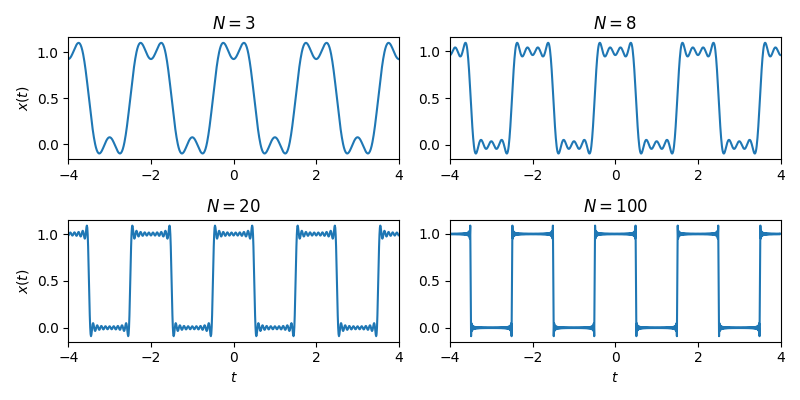
\includegraphics[height=5cm]{4.1.5-2.png}
\end{figure}

\begin{python}
t  = np.arange(-4, 4, 0.01)
x1 = np.full_like(t, 0.5, dtype=np.float32)
N = 3
for n in range(1,N+1,2):
    x1 += 2/n/np.pi * np.sin(n*np.pi/2) * np.cos(n*np.pi*t)
    pass

axs[0][0].plot(t, x1)
\end{python}

\begin{tcolorbox}
由于时域方波有不连续点,不满足狄利克雷收敛条件,所以在这些间断点,傅里叶级数和原函数有9\%的误差,称为{\bf Gibbs现象}。
\end{tcolorbox}

~

\begin{example}
假设如下图信号,求傅里叶级数,当$T=2,a=0.5$时,用Python作图验证。
\begin{figure}[h]
\centering
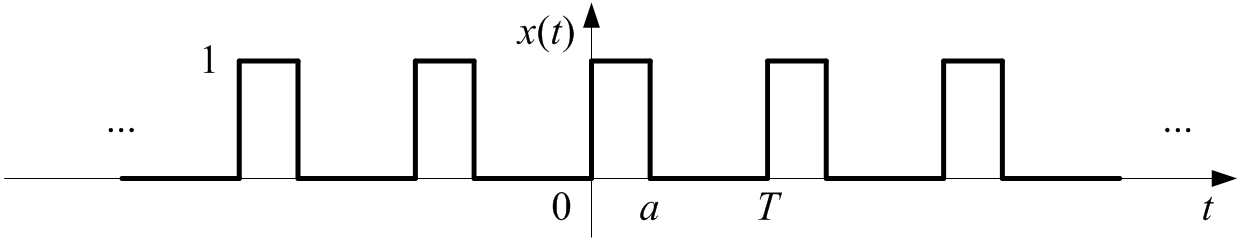
\includegraphics[height=2cm]{4.1.5-3.png}
\end{figure}
\end{example}

计算傅里叶系数:
\begin{align*}
&C_0=\frac{1}{T}\int_{-\frac{T}{2}}^{\frac{T}{2}}{x\left( t \right) dt}=\frac{1}{T}\int_0^a{dt}=\frac{a}{T} \\
&C_n=\frac{1}{T}\int_{-\frac{T}{2}}^{\frac{T}{2}}{x\left( t \right) e^{-i\omega _nt}dt}=\frac{1}{T}\int_0^a{e^{-in\frac{2\pi}{T}t}dt} =\frac{i}{2n\pi}\left( e^{-\frac{i2an\pi}{T}}-1 \right)
\end{align*}
得傅里叶级数:
\[
x\left( t \right) =C_0+\sum_{n=\pm 1}^{\pm \infty}{\left[ C_n\cdot e^{in\frac{2\pi}{T}t} \right]}=\frac{a}{T}+\sum_{n=1}^{+\infty}{\frac{\sin \frac{2n\pi t}{T}-\sin \frac{2n\pi \left( t-a \right)}{T}}{n\pi}}
\]
\begin{figure}[h]
\centering
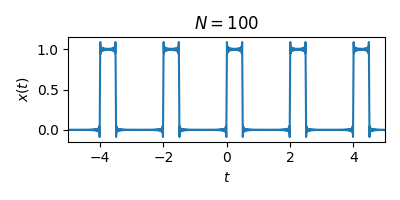
\includegraphics[height=3cm]{4.1.5-4.png}
\end{figure}

~

\begin{example}
设如下图信号,求傅里叶级数,用Python作图验证。
\begin{figure}[h]
\centering
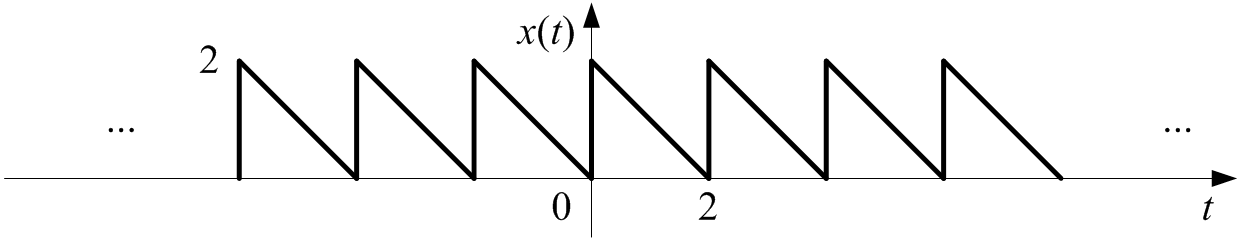
\includegraphics[height=2cm]{4.1.5-5.png}
\end{figure}
\end{example}

显然,信号有$x\left( t \right) =2-t,T=2$,计算傅里叶系数:
\begin{align*}
&C_0=\frac{1}{T}\int_{-\frac{T}{2}}^{\frac{T}{2}}{x\left( t \right) dt}=\frac{1}{2}\int_0^2{\left( 2-t \right) dt}=1 \\
&C_n=\frac{1}{T}\int_{-\frac{T}{2}}^{\frac{T}{2}}{x\left( t \right) e^{-i\omega _nt}dt}=\frac{1}{2}\int_0^2{\left( 2-t \right) e^{-i\omega _nt}dt}=\frac{1-i2\omega _n-e^{-i2\omega _n}}{2{\omega _n}^2}
\end{align*}
得傅里叶级数:
\begin{align*}
x\left( t \right) &=C_0+\sum_{n=\pm 1}^{\pm \infty}{\left[ C_n\cdot e^{in\omega _nt} \right]} \\
&=1+\sum_{n=1}^{+\infty}{\frac{\cos \left( n\pi t \right) +2n\pi \sin \left( n\pi t \right) -\cos \left( n\pi \left( t-2 \right) \right)}{\left( n\pi \right) ^2}}
\end{align*}
\begin{figure}[h]
\centering
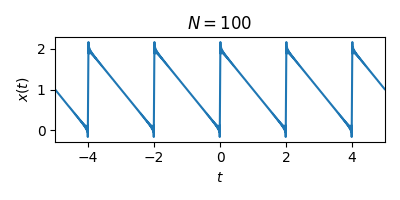
\includegraphics[height=3cm]{4.1.5-6.png}
\end{figure}






\newpage
\section{非周期信号的傅里叶变换}

本节介绍非周期信号的傅里叶变换。
傅里叶变换是频域分析的重要方法,也是各种其他变换的基础。

本节要点:
\begin{itemize}
    \item 深入理解傅里叶变换及其物理意义;
    \item 理解傅里叶变换的量纲;
    \item 理解傅里叶变换的条件;
    \item 熟悉傅里叶变换的极坐标形式;
    \item 了解傅里叶级数和傅里叶变换的关系。
\end{itemize}

\begin{tcolorbox}
建议和《微积分》课程中的傅里叶积分对比着学习!
\end{tcolorbox}

%============================================================
\subsection{傅里叶变换的概念}

\begin{definition}[傅里叶变换]
若非周期信号$x\left( t \right) $满足:
\begin{itemize}
    \item 任一有限区域上满足狄利克雷收敛条件,
    \item 整个实数域绝对可积,即$\int_{-\infty}^{+\infty}{\left| x\left( t \right) \right|dt}$收敛,
\end{itemize}
则有:
\[
x\left( t \right) =\frac{1}{2\pi}\int_{-\infty}^{+\infty}{\left[ \int_{-\infty}^{+\infty}{x\left( t \right) e^{-i\omega t}dt} \right] e^{i\omega t}d\omega}
\]
对$x\left( t \right) $所有的连续点成立,称为{\bf $x\left( t \right) $的傅里叶积分},在间断点$t_0$处,可以用$\frac{1}{2}\left[ x\left( {t_0}^+ \right) +x\left( {t_0}^- \right) \right] $代替。
同时称$\int_{-\infty}^{+\infty}{x\left( t \right) e^{-i\omega t}dt}$为{\bf 信号$x\left( t \right) $的傅里叶变换}(Fourier transform,FT),记为$X\left( \omega \right) $即:
\[
X\left( \omega \right) =\int_{-\infty}^{+\infty}{x\left( t \right) e^{-i\omega t}dt}
\]
相应地称
\[
x\left( t \right) =\frac{1}{2\pi}\int_{-\infty}^{+\infty}{X\left( \omega \right) e^{i\omega t}d\omega}
\]
为{\bf 傅里叶逆变换}。
信号及其傅里叶变换形式通常记为:
\[
x\left( t \right) \overset{\mathscr{F}}{\leftrightarrow}X\left( \omega \right)
\]
\end{definition}

傅里叶变换是针对非周期信号而言的,所以没有基频这个概念,频率是一片连续的范围,与之相对的是周期信号的傅里叶级数的频率是无穷个离散值,可以想象成“连续谱”vs“线状谱”,傅里叶级数中的系数也从离散的$C_n$变成连续的$X\left( \omega \right) $。

如果信号在时域占满整个实数域$\mathbb{R} $,则对应傅里叶变换的频率在一个区间$\left( -\omega _0,+\omega _0 \right) $,相反,如果信号在时域是一个区间$\left( t_1,t_2 \right) $,则在频域将占满整个频率$\mathbb{R} $,即信号要么时域有限,要么频域有限,通常来讲,一般物理信号都是时域有限信号,所以是频域无限。

傅里叶变换和逆变换的对称性可知,只要信号能有傅里叶变换,则必有其傅里叶变换绝对可积,即$\int_{-\infty}^{+\infty}{\left| X\left( \omega \right) \right|d\omega}$收敛。

%============================================================
\subsection{傅里叶变换的量纲}

从定义式易得$X\left( \omega \right) $的量纲是信号的量纲乘以时间的量纲,或者说是信号的量纲除以频率的量纲$\mathrm{D}_x\cdot \mathrm{Hz}^{-1}$,这点是和傅里叶级数的区别。
{\bf $X\left( \omega \right) $的物理意义可以理解为单位频率的信号,或者说信号的频率密度。}
有些教材中会使用“信号分布在低频”这样的说法!

%============================================================
\subsection{傅里叶级数和傅里叶变换对比}

傅里叶级数和傅里叶变换的对比见下表:

\begin{table}[h]
\centering
% \caption{表头}
\begin{tabular}{ccc}
    \toprule
    & 傅里叶级数 & 傅里叶变换\\
    \midrule
    目标函数 & 周期函数 & 非周期函数\\
    展开 & $x\left( t \right) =\sum_{n=-\infty}^{+\infty}{\left( C_ne^{i\omega _nt} \right)}$ & $x\left( t \right) =\frac{1}{2\pi}\int_{-\infty}^{+\infty}{X\left( \omega \right) e^{i\omega t}d\omega}$\\
    角频 & 离散值,$\omega _n=n\omega _0=n\frac{2\pi}{T}$ & 连续值,$\omega \in \mathbb{R} $\\
    系数 & $C_n=\frac{1}{T}\int_{-\frac{T}{2}}^{\frac{T}{2}}{x\left( t \right) e^{-i\omega _nt}dt}$ & $X\left( \omega \right) =\int_{-\infty}^{+\infty}{x\left( t \right) e^{-i\omega t}dt}$\\
    \bottomrule
\end{tabular}
\end{table}

总之,对于周期信号的傅里叶级数,角频和系数的取值都是离散值,对于非周期信号的傅里叶变换,角频和系数的取值都是连续值。
这点可以类比为离散信号和连续信号。

%============================================================
\subsection{傅里叶变换的极坐标形式}

由于傅里叶变换有复指数项,所以结果一般是一个复数函数,可以变成极坐标形式:
\begin{align*}
X\left( \omega \right) &=\int_{-\infty}^{+\infty}{x\left( t \right) e^{-i\omega t}dt} \\
&=\int_{-\infty}^{+\infty}{x\left( t \right) \cos \left( \omega t \right) dt}+i\int_{-\infty}^{+\infty}{-x\left( t \right) \sin \left( \omega t \right) dt} \\
&=R\left( \omega \right) +iI\left( \omega \right)
\end{align*}
于是:
\begin{align*}
&\therefore \begin{cases}
	X\left( \omega \right) =\sqrt{R^2\left( \omega \right) +I^2\left( \omega \right)}\\
	\angle X\left( \omega \right) =\mathrm{arc}\tan \frac{I\left( \omega \right)}{R\left( \omega \right)}\\
\end{cases} \\
&\therefore X\left( \omega \right) =\left| X\left( \omega \right) \right|\cdot e^{i\angle X\left( \omega \right)}
\end{align*}
可以做类比:
\begin{itemize}
    \item $X\left( \omega \right) $:相当于傅里叶级数中的复指系数$C_n$;
    \item $\left| X\left( \omega \right) \right|$:相当于傅里叶级数中的幅度$A_n$;
    \item $\angle X\left( \omega \right) $:相当于傅里叶级数中的相位$\varphi _n$。
\end{itemize}

%============================================================
\subsection{广义傅里叶变换}

对于有些函数,如$x\left( t \right) =1,x\left( t \right) =\sin t$等,由于不满足狄利克雷条件,没有严格意义上的傅里叶变换,但可以通过单位冲激结合傅里叶变换的性质定义广义傅里叶变换。

单位冲激的傅里叶变换:
\begin{align*}
&\because \int_{-\infty}^{+\infty}{\delta \left( t \right) e^{i\omega t}dt}=\int_{-\infty}^{+\infty}{\delta \left( t \right) dt}=1 \\
&\therefore \delta \left( t \right) \leftrightarrow 1
\end{align*}
通过Duality,$x\left( t \right) =1$的广义傅里叶变换:
\[
1\leftrightarrow 2\pi \delta \left( \omega \right)
\]
以上只是一个例子,通过$\delta \left( t \right) $的傅里叶变换和傅里叶变换的性质,我们可以求得很多函数的广义傅里叶变换。

%============================================================
\subsection{傅里叶变换的性质}

{\bf 奇偶性}

如果$x\left( t \right) $是偶函数,则其傅里叶变换是实函数,如果$x\left( t \right) $是奇函数,则其傅里叶变换是纯虚函数,除此之外,一般傅里叶变换是复变函数。
\begin{align*}
&x\left( t \right) \text{ is even} \quad \Rightarrow \quad X\left( \omega \right) =\int_{-\infty}^{+\infty}{x\left( t \right) \cos \left( \omega t \right) dt} \\
&x\left( t \right) \text{ is odd} \quad \Rightarrow \quad X\left( \omega \right) =-i\int_{-\infty}^{+\infty}{x\left( t \right) \sin \left( \omega t \right) dt}
\end{align*}

{\bf 线性性}(由于积分的线性性,不证自明)
\[
ax\left( t \right) +by\left( t \right) \leftrightarrow aX\left( \omega \right) +bY\left( \omega \right)
\]

{\bf 时移性、频移性}(积分变量做一个变换即可证明)
\begin{align*}
&x\left( t-t_1 \right) \leftrightarrow X\left( \omega \right) e^{i\omega t_1} \\
&e^{i\omega t_1}x\left( t \right) \leftrightarrow X\left( \omega -\omega _1 \right)
\end{align*}

“时移性”表示信号在时域的延迟对傅里叶变换的结果是所有频率分量都慢了一个相位(即旋转),大小不变。
物理上讲,因为时间起点是人为设定的,所以信号的时移应具有FT的某种不变性。

{\bf 时展性}(积分变量做一个变换即可证明)
\begin{align*}
&x\left( at \right) \leftrightarrow \frac{1}{a}X\left( \frac{\omega}{a} \right) \\
&x\left( -t \right) \leftrightarrow -X\left( -\omega \right) =\bar{X}\left( \omega \right)
\end{align*}

“时展性”表示对时域的尺度变换对导致频域的尺度“相反地”变换。
这个容易理解,时域尺缩表示信号变化加快,自然频率尺扩,即高频分量增加。

{\bf 三角律}(频移性结合欧拉公式即可证明)
\begin{align*}
&x\left( t \right) \cos \omega _1t\leftrightarrow \frac{1}{2}\left[ X\left( \omega +\omega _1 \right) +X\left( \omega -\omega _1 \right) \right] \\
&x\left( t \right) \sin \omega _1t\leftrightarrow \frac{i}{2}\left[ X\left( \omega +\omega _1 \right) -X\left( \omega -\omega _1 \right) \right]
\end{align*}

{\bf 时域的微分和积分、频域的微分}
\begin{align*}
&\frac{d^nx\left( t \right)}{dt^n}\leftrightarrow \left( i\omega \right) ^n\cdot X\left( \omega \right) \\
&\int_{-\infty}^t{x\left( \tau \right) d\tau}\leftrightarrow \frac{1}{i\omega}\cdot X\left( \omega \right) \\
&\left( \frac{t}{i} \right) ^n\cdot x\left( t \right) \leftrightarrow \frac{d^nX\left( \omega \right)}{d\omega ^n}
\end{align*}

时域微分公式的前提是$\underset{t\rightarrow \pm \infty}{\lim} x\left( t \right) =0$。
时域积分通常来讲只有广义傅里叶变换,$\int_{-\infty}^t{x\left( \tau \right) d\tau}\leftrightarrow \frac{1}{i\omega}\cdot X\left( \omega \right) +\pi X\left( 0 \right) \delta \left( \omega \right) $。
特别地当时域信号没有直流分量时($X\left( 0 \right) =0$),才能得到上述公式。

{\bf 卷积性}
\begin{align*}
&x\left( t \right) \ast y\left( t \right) \leftrightarrow X\left( \omega \right) \cdot Y\left( \omega \right) \\
&x\left( t \right) \cdot y\left( t \right) \leftrightarrow \frac{1}{2\pi}\left[ X\left( \omega \right) \ast Y\left( \omega \right) \right]
\end{align*}

{\bf Parseval定理}
\begin{align*}
&\int_{-\infty}^{+\infty}{x\left( t \right) y\left( t \right) dt}=\frac{1}{2\pi}\int_{-\infty}^{+\infty}{\bar{X}\left( \omega \right) Y\left( \omega \right) d\omega} \\
&\int_{-\infty}^{+\infty}{x^2\left( t \right) dt}=\frac{1}{2\pi}\int_{-\infty}^{+\infty}{\left| X\left( \omega \right) \right|^2d\omega}
\end{align*}

{\bf Duality}
\[
X\left( t \right) \leftrightarrow 2\pi x\left( -\omega \right)
\]

%============================================================
\subsection{例}

\begin{example}
若有指数信号$x\left( t \right) =e^{-bt}u\left( t \right) $,求其傅里叶变换。
\end{example}

\begin{align*}
X\left( \omega \right) &=\int_{-\infty}^{+\infty}{x\left( t \right) e^{-i\omega t}dt}=\int_{-\infty}^{+\infty}{e^{-\left( b+i\omega \right) t}dt} \\
&=-\frac{1}{b+i\omega}\left[ \left. e^{-\left( b+i\omega \right) t} \right|_{0}^{+\infty} \right]
\end{align*}
当$b>0$时,有$\underset{t\rightarrow +\infty}{\lim} e^{-bt}=0$,则:
\[
X\left( \omega \right) =\frac{1}{b+i\omega}
\]
傅里叶变换是一个复数。
当$b\leqslant 0$时,$e^{-bt}$不收敛,信号不满足绝对可积条件,无傅里叶变换。

~

\begin{example}
若如下单方波信号,求其傅里叶变换,并分析脉宽和傅里叶变换之间的关系。
\[
p_{\tau}\left( t \right) =\begin{cases}
	1,t\in \left[ -\frac{\tau}{2},\frac{\tau}{2} \right]\\
	0,t\notin \left[ -\frac{\tau}{2},\frac{\tau}{2} \right]\\
\end{cases}
\]
\end{example}

先求傅里叶变换:
\begin{align*}
X\left( \omega \right) &=\int_{-\infty}^{+\infty}{x\left( t \right) e^{-i\omega t}dt}=\int_{-\frac{\tau}{2}}^{\frac{\tau}{2}}{e^{-i\omega t}dt} \\
&=\frac{1}{-i\omega}\left. e^{-i\omega t} \right|_{-\frac{\tau}{2}}^{\frac{\tau}{2}}=\frac{1}{-i\omega}\left( e^{-i\omega \frac{\tau}{2}}-e^{i\omega \frac{\tau}{2}} \right) \\
&=\frac{2}{\omega}\sin \frac{\omega \tau}{2}=\tau \frac{\sin \frac{\omega \tau}{2}}{\frac{\omega \tau}{2}}=\tau \mathrm{sinc}\frac{\omega \tau}{2\pi}
\end{align*}
由于信号是一个偶信号,傅里叶变换的结果是一个实数,它的相位永远只有0°和180°两个值。

以$\tau =0.5,\tau =1.5$两个脉宽的单方波信号为例,幅频图和相频图如下。

\begin{python}
w   = np.arange(-10*np.pi, 10*np.pi, 0.01)
tau = 0.5; X1 = tau * np.sinc(w*tau / 2 / np.pi)
tau = 1.5; X2 = tau * np.sinc(w*tau / 2 / np.pi)

plot_mag_phs(w, np.abs(X1), np.angle(X1, deg=True),
             axs[0][0], axs[1][0], title=r'$\tau =0.5$', ...)
plot_mag_phs(w, np.abs(X2), np.angle(X2, deg=True),
             axs[0][1], axs[1][1], title=r'$\tau =1.5$', ...)
\end{python}

\begin{figure}[h]
\centering
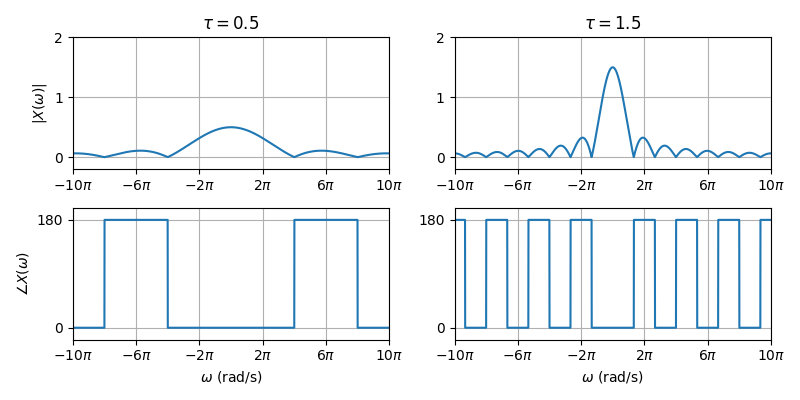
\includegraphics[height=5cm]{4.2.7-1.png}
\end{figure}

注意:
\begin{itemize}
    \item 所有图像的横坐标是角频$\omega $,单位是$\mathrm{rad}\cdot \mathrm{s}^{-1}$,为方便用弧度表示;
    \item $\underset{\tau \rightarrow 0}\lim p_{\tau}\left( t \right) =1,\underset{\tau \rightarrow 0}\lim X\left( \omega \right) =\delta \left( \omega \right) $。
\end{itemize}



\newpage
\section{Python应用——傅里叶变换函数}

本章的一个重点是能够将一个时域图形变换成傅里叶频谱并分析。
本节编写Python傅里叶变换函数,并借助Python快捷地获得傅里叶变换。

本节要点:
\begin{itemize}
    \item 学会Python编写傅里叶变换函数;
    \item 掌握分析方法。
\end{itemize}

%============================================================
\subsection{Python傅里叶变换函数}

由于Python没有傅里叶变换的函数,Numpy和Scipy都只有FFT,所以编写一个傅里叶变换的函数。

根据傅里叶变换公式my\_fourier编写如下函数:
\[
X\left( \omega \right) =\int_{-\infty}^{+\infty}{x\left( t \right) e^{-i\omega t}dt}
\]

\begin{python}
def my_fourier(
        x:np.ndarray, t:np.ndarray,
        w_range:tuple=(-5*np.pi, 5*np.pi), num:int=500
        ) -> tuple:

    w = np.linspace(w_range[0], w_range[1], num+1)
    F = np.zeros_like(w, dtype=np.complex64)
    dt = t[1] - t[0]

    for n in range(F.size):
        F[n] = np.dot(x, np.exp(0-w[n]*t*1.0j)) * dt
        pass

    return (F, w)
\end{python}

参数:
\begin{itemize}
    \item x:np.ndarray类型,表示信号$x\left( t \right) $的值;
    \item t:np.ndarray类型,表示信号$x\left( t \right) $的时间;
    \item w\_range:元组类型,表示$\omega $的取值范围,需要原点对称;
    \item num:整数类型,表示$\omega $的离散个数,也即$\omega $的采样个数。
\end{itemize}

函数流程:
\begin{enumerate}
    \item 首先根据w\_range和num生成w,我们做的傅里叶变换就在这个范围内,也即$\omega $的采样点,0点对称;
    \item 初始化傅里叶离散点,注意F的类型是np.complex64;
    \item 循环,核心是做积分;
    \item 返回(F,w)表示$F\left( \omega \right) ,\omega $。
\end{enumerate}

%============================================================
\subsection{分析方法}

通常有一类问题是已知一个连续信号的时域波形图,要分析它的频域。借助我们的函数,一般步骤如下:
\begin{enumerate}
    \item 根据图形写出连续信号的时域函数;
    \item 用my\_fourier()求傅里叶变换;
    \item 用Matplotlib画出幅频图和相频图分析。
\end{enumerate}

%============================================================
\subsection{例}

\begin{example}
假设有信号$x\left( t \right) =p_2\left( t \right) $,用Python计算傅里叶变换,并作图。
\end{example}

用Python求解傅里叶变换并作图:

\begin{python}
t    = np.arange(-20, 20, 0.01)
x    = np.where(t<-1, 0, np.where(t>1, 0, 1))
X, w = my_fourier(x, t, w_range=(-6*np.pi, 6*np.pi), num=1000)

axs[0].plot(t, x)
plot_mag_phs(w, np.abs(X), np.angle(X, deg=True), ...)
\end{python}

\begin{figure}[h]
\centering
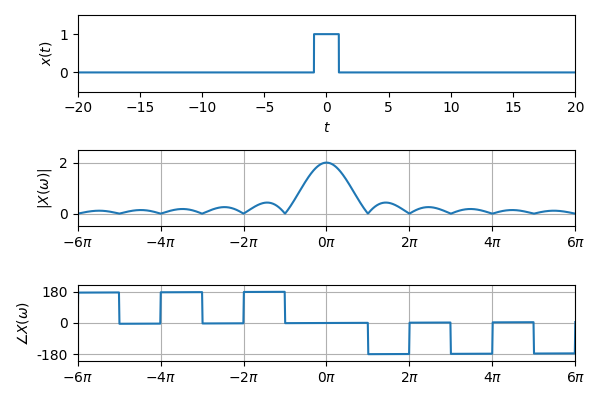
\includegraphics[height=5cm]{4.3.3-1.png}
\end{figure}

~

\begin{example}
设函数有如下图形,用Python分析傅里叶变换。
\begin{figure}[h]
\centering
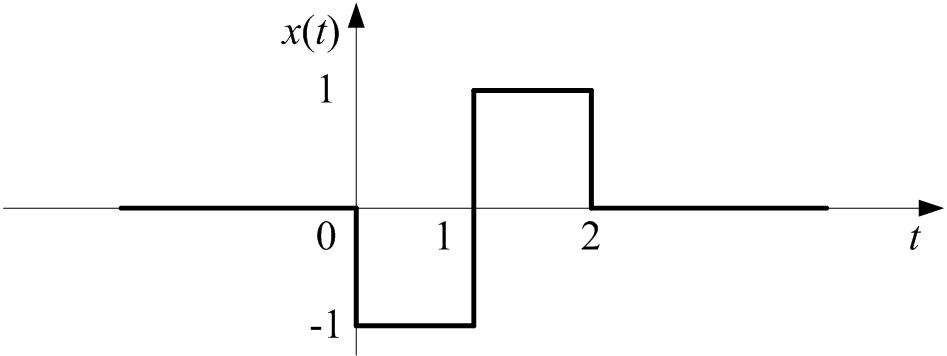
\includegraphics[height=2.5cm]{4.3.3-2.png}
\end{figure}
\end{example}

根据图形得到时域函数$x\left( t \right) =-u\left( t \right) +2u\left( t-1 \right) -u\left( t-2 \right) $,用Python求解傅里叶变换并作图:

\begin{python}
t    = np.arange(-20, 20, 0.01)
x    = np.where(t<0, 0, np.where(t<1, -1, np.where(t<2, 1, 0)))
X, w = my_fourier(x, t, w_range=(-6*np.pi, 6*np.pi))

axs[0].plot(t, x)
plot_mag_phs(w, np.abs(X), np.angle(X, deg=True), ...)
\end{python}

\begin{figure}[h]
\centering
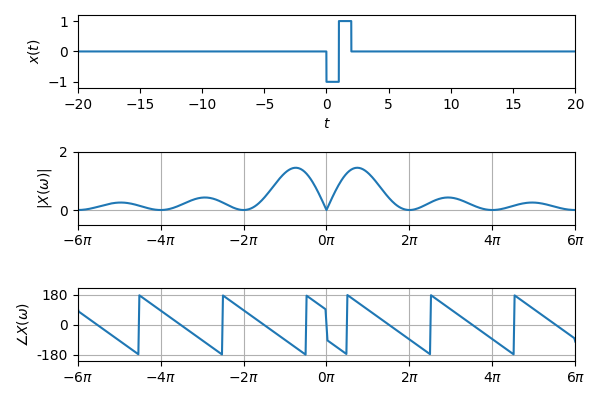
\includegraphics[height=5cm]{4.3.3-3.png}
\end{figure}

~

\begin{example}
设函数有如下图形,用Python分析傅里叶变换。
\begin{figure}[h]
\centering
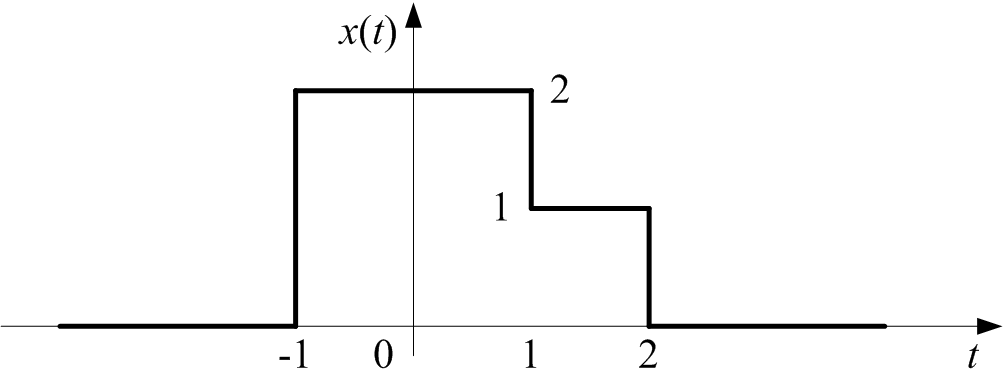
\includegraphics[height=2.5cm]{4.3.3-4.png}
\end{figure}
\end{example}

\begin{figure}[h]
\centering
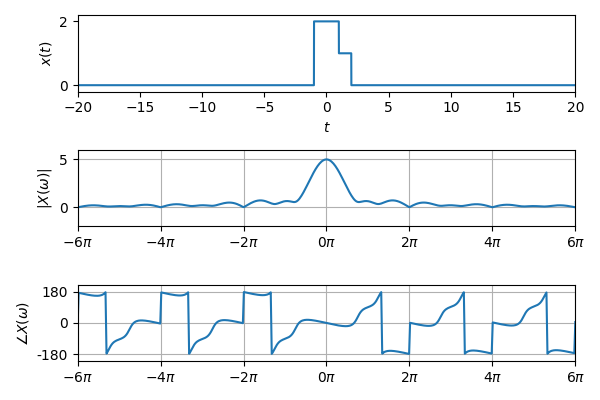
\includegraphics[height=5cm]{4.3.3-5.png}
\end{figure}

根据图形得到时域函数$x\left( t \right) =2u\left( t+1 \right) -u\left( t-1 \right) -u\left( t-2 \right) $,用Python求解傅里叶变换并作图:

\begin{python}
t    = np.arange(-20, 20, 0.01)
x    = np.where(t<-1, 0, np.where(t<1, 2, np.where(t<2, 1, 0)))
X, w = my_fourier(x, t, w_range=(-6*np.pi, 6*np.pi))

axs[0].plot(t, x)
plot_mag_phs(w, np.abs(X), np.angle(X, deg=True), ...)
\end{python}






\newpage
\section{本章小结}

傅里叶是频域分析的基础,必须深刻理解其含义,并熟练掌握计算方法。
时刻记住,数学本质上,傅里叶变换是函数的空间变换,将原本$x$空间的函数映射到三角函数(或指数函数)空间。
在信号与系统角度,具象化为时域到频域的变换,将原本对时间$t$的函数变换成对频率$\omega $的函数:
\[
\begin{array}{l}
	x=x\left( t \right)\\
	t\in \mathbb{R}\\
	x\in \mathbb{R}\\
\end{array} \quad \rightarrow \quad \begin{array}{l}
	X=X\left( \omega \right)\\
	\omega \in \mathbb{R}\\
	X\in \mathbb{C}\\
\end{array}
\]
一般来讲,$X\left( \omega \right) $的值域是复数,大小表示频率的振幅,角度表示频率的相位。

最后,需要特别注意$X\left( \omega \right) $的量纲$\mathrm{D}_x\cdot \mathrm{Hz}^{-1}$,及其物理意义“单位频率的信号,或者说信号的频率密度”。










\chapter{系统的频率分析}

上一章介绍了傅里叶变换,也介绍了信号的傅里叶变换和信号的频域分析。

本章用傅里叶变换分析系统。
首先分析频域角度上的系统响应,即“系统的频率响应”,给出“频率响应函数”概念。
再以RC电路为例,在频域角度分析系统特性。
最后用频率响应函数定义理想滤波器。

本章要点:
\begin{itemize}
    \item 系统的频率响应。
    \item 频率响应函数。
    \item 理想滤波器。
    \item Nuquist采样定理
\end{itemize}

\newpage
\section{系统的频率响应}

本节在频域角度,讨论系统如何对输入作用产生输出,介绍系统的频域响应定理与频率响应函数,并给出快速求解系统频率响应函数的方法。

本节要点:
\begin{itemize}
    \item 掌握系统频率响应的概念;
    \item 理解频率响应函数的概念和意义;
    \item 掌握频率响应函数的求解方法。
\end{itemize}

%============================================================
\subsection{频域响应定理与频率响应函数}

\begin{theorem}[系统的频域响应定理]
若一个零状态LTI系统满足绝对稳定的条件,即$\int_{-\infty}^{+\infty}{\left| h\left( t \right) \right|dt}$收敛,则系统对于任意非周期信号$x\left( t \right) $在时域的输出可以表示为卷积:
\[
y\left( t \right) =x\left( t \right) \ast h\left( t \right)
\]
在频域的输出可以表示为傅里叶变换的乘积:
\[
Y\left( \omega \right) =X\left( \omega \right) \cdot H\left( \omega \right)
\]
\begin{itemize}
    \item $x\left( t \right) ,y\left( t \right) $:输入输出信号的时域表达式;
    \item $h\left( t \right) $:系统的冲激响应;
    \item $X\left( \omega \right) ,Y\left( \omega \right) $:输入输出信号的傅里叶变换;
    \item $H\left( \omega \right) $:{\bf 系统的频率响应函数}(frequency response function),或称{\bf 系统函数}(system function),即$h\left( t \right) $的傅里叶变换。
\end{itemize}
\end{theorem}

这表明,一个绝对稳定的LTI系统对任何输入的信号,系统会单独作用其各个频率分量的幅度和相位:
\begin{align*}
&\left| Y\left( \omega \right) \right|=\left| X\left( \omega \right) \right|\cdot \left| H\left( \omega \right) \right| \\
&\angle Y\left( \omega \right) =\angle X\left( \omega \right) +\angle H\left( \omega \right)
\end{align*}
以简单的正弦信号为例,若信号$x\left( t \right) =A\cos \left( \omega _0t+\varphi \right) $,则输出:
\[
y\left( t \right) =A\left| H\left( \omega _0 \right) \right|\cos \left( \omega _0t+\varphi +\angle H\left( \omega _0 \right) \right)
\]
\begin{itemize}
    \item 若系统是无源系统,则$\left| H\left( \omega _0 \right) \right|\leqslant 1$,表示衰减,若系统为有源系统,对应$\left| H\left( \omega _0 \right) \right|>1$,表示放大;
    \item 由于因果性,系统都会将相位往后拉$\angle H\left( \omega _0 \right) $。
\end{itemize}

从定义上来说,$H\left( \omega \right) $是系统的$h\left( t \right) $的傅里叶变换,$h\left( t \right) $是系统对$\delta \left( t \right) $的响应。
由于$\delta \left( t \right) \leftrightarrow 1$,所以从频域上看,$H\left( \omega \right) $是系统对于输入$X\left( \omega \right) =1$的响应。
明白了这一点,也就明白了为什么$H\left( \omega \right) $会被称为“频率响应函数”,指的是系统对各个频率的响应。

%============================================================
\subsection{时域响应和频域响应}

至此,时域响应和频域响应讨论完毕。

在时域我们通过卷积模型描述系统,系统的输出为冲激响应对输入进行卷积运算的结果,不同的系统表现为不同的$h\left( t \right) $。
在频域我们通过傅里叶变换描述系统,输出为频率响应和输入信号的乘积,不同的系统表现为不同的$H\left( \omega \right) $。
无论是卷积模型还是傅里叶变换,本质上都是系统微分方程的反映,是微分方程的冲激函数的解在时域和频域的不同体现。
\[
y\left( t \right) \overset{h\left( t \right) \leftrightarrow H\left( \omega \right)}{=}\begin{cases}
	x\left( t \right) \ast h\left( t \right)\\
	\mathscr{F} ^{-1}\left[ H\left( \omega \right) \cdot X\left( \omega \right) \right]\\
\end{cases}
\]

%============================================================
\subsection{频率响应函数的求解}

\begin{tcolorbox}
系统的频率响应函数可以从定义上求解,但这涉及求解微分方程,特别是高阶的微分方程,几乎无解。
这里给出一个求解的方法。
\end{tcolorbox}

若有限维度LTI系统的微分方程如下:
\[
y^{\left( n \right)}\left( t \right) +\sum_{k=0}^{n-1}{A_ky^{\left( k \right)}\left( t \right)}=\sum_{k=0}^m{B_kx^{\left( k \right)}\left( t \right)}
\]
根据傅里叶变换的导数性质$\frac{d^nx\left( t \right)}{dt^n}\leftrightarrow \left( i\omega \right) ^n\cdot X\left( \omega \right) $,两边取傅里叶变换:
\[
\left( i\omega \right) ^nY\left( \omega \right) +\sum_{k=0}^{n-1}{A_k\left( i\omega \right) ^kY\left( \omega \right)}=\sum_{k=0}^m{B_k\left( i\omega \right) ^kX\left( \omega \right)}
\]
整理后得到:
\[
H\left( \omega \right) =\frac{\sum_{k=0}^m{B_k\left( i\omega \right) ^k}}{\left( i\omega \right) ^n+\sum_{k=0}^{n-1}{A_k\left( i\omega \right) ^k}}
\]

\begin{tcolorbox}
由于$i$代表虚数符号,所以进入到傅里叶章节后用$k$作为连加的序数。
\end{tcolorbox}

%============================================================
\subsection{例}

\begin{example}
如下RC电路,设电压源为输入,电容两端电压为输出,分析系统的频率响应函数。
\begin{figure}[h]
\centering
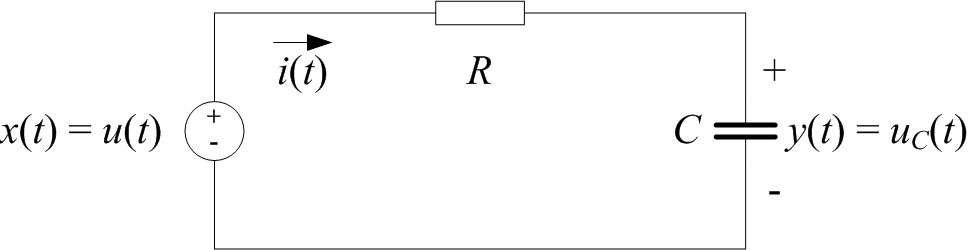
\includegraphics[height=2cm]{1.5.1-1.png}
\end{figure}
\end{example}

根据之前对该电路的分析,系统微分方程有:
\[
\frac{dy}{dt}+\frac{1}{RC}y=\frac{1}{RC}x
\]
直接运用上面的推导结论,有:
\[
H\left( \omega \right) =\frac{\sum_{k=0}^m{B_k\left( i\omega \right) ^k}}{\left( i\omega \right) ^n+\sum_{k=0}^{n-1}{A_k\left( i\omega \right) ^k}}=\frac{\frac{1}{RC}\left( i\omega \right) ^0}{\left( i\omega \right) ^1+\frac{1}{RC}\left( i\omega \right) ^0}=\frac{\frac{1}{RC}}{i\omega +\frac{1}{RC}}
\]
用最原始的方法,求解微分方程->求解冲激响应->获得频率响应函数。
求解微分方程及冲激响应:
\begin{align*}
&y=\frac{1}{RC}e^{-\frac{t}{RC}}\int_0^t{e^{\frac{\tau}{RC}}x\left( \tau \right) d\tau} \\
&h=\left. y \right|_{x=\delta}=\frac{1}{RC}e^{-\frac{t}{RC}}\int_0^t{e^{\frac{\tau}{RC}}\delta \left( \tau \right) d\tau}=\frac{1}{RC}e^{-\frac{t}{RC}}
\end{align*}
求解频率响应函数:
\begin{align*}
&\because e^{-bt}u\left( t \right) \leftrightarrow \frac{1}{b+i\omega} \\
&\therefore H\left( \omega \right) =\frac{1}{RC}\frac{1}{\frac{1}{RC}+i\omega}
\end{align*}

~

\begin{example}
设有弹簧减震装置,系统的微分方程为$x-D\frac{dy}{dt}-Ky=M\frac{d^2y}{dt^2}$,求解其频率响应函数。
\end{example}

先将方程化为:
\[
\frac{d^2y}{dt^2}+\frac{D}{M}\frac{dy}{dt}+\frac{K}{M}y=\frac{1}{M}x
\]
运用本节的方法:
\begin{align*}
H\left( \omega \right) &=\frac{\sum_{k=0}^m{B_k\left( i\omega \right) ^k}}{\left( i\omega \right) ^n+\sum_{k=0}^{n-1}{A_k\left( i\omega \right) ^k}}=\frac{\frac{1}{M}}{\left( i\omega \right) ^2+\left( i\omega \right) \frac{D}{M}+\frac{K}{M}} \\
&=\frac{1}{-M\omega ^2+iD\omega +k}
\end{align*}






\newpage
\section{理想滤波器}

本节介绍理想滤波器的概念,随后讨论理想低通的可能性。

本节要点:
\begin{itemize}
    \item 理解4类理想滤波器;
    \item 从因果律理解低通滤波器。
\end{itemize}

%============================================================
\subsection{理想滤波器的幅频和相频要求}

幅频上考察,理想滤波器分为:
\begin{itemize}
    \item {\bf 低通}(lowpass),$\left| H\left( \omega \right) \right|=1,\omega \in \left[ -B,B \right] $,并称$B$为{\bf 滤波器带宽};
    \item {\bf 高通}(highpass),$\left| H\left( \omega \right) \right|=1,\omega \notin \left[ -B,B \right] $;
    \item {\bf 带通}(bandpass),$\left| H\left( \omega \right) \right|=1,\omega \in \left[ -B_1,B_2 \right] $,并称$B_2-B_1$为{\bf 滤波器带宽};
    \item {\bf 带阻}(bandstop),$\left| H\left( \omega \right) \right|=1,\omega \notin \left[ -B_1,B_2 \right] $。
\end{itemize}
理想滤波器对于通带没有任何衰减,对于禁带则完全衰减。

相频上,理想滤波器必须满足频率的线性性:
\[
\angle H\left( \omega \right) =-a\omega \qquad a\geqslant 0
\]
为满足因果律,必须$a\geqslant 0$,使得输出相对输入是延时的,才能使任何频率的正弦波没有频率扭曲。
\[
y\left( t \right) =A\left| H\left( \omega \right) \right|\cos \left( \omega _0t-a\omega _0 \right) =A\left| H\left( \omega \right) \right|\cos \left[ \omega _0\left( t-a \right) \right]
\]
\begin{figure}[h]
\centering
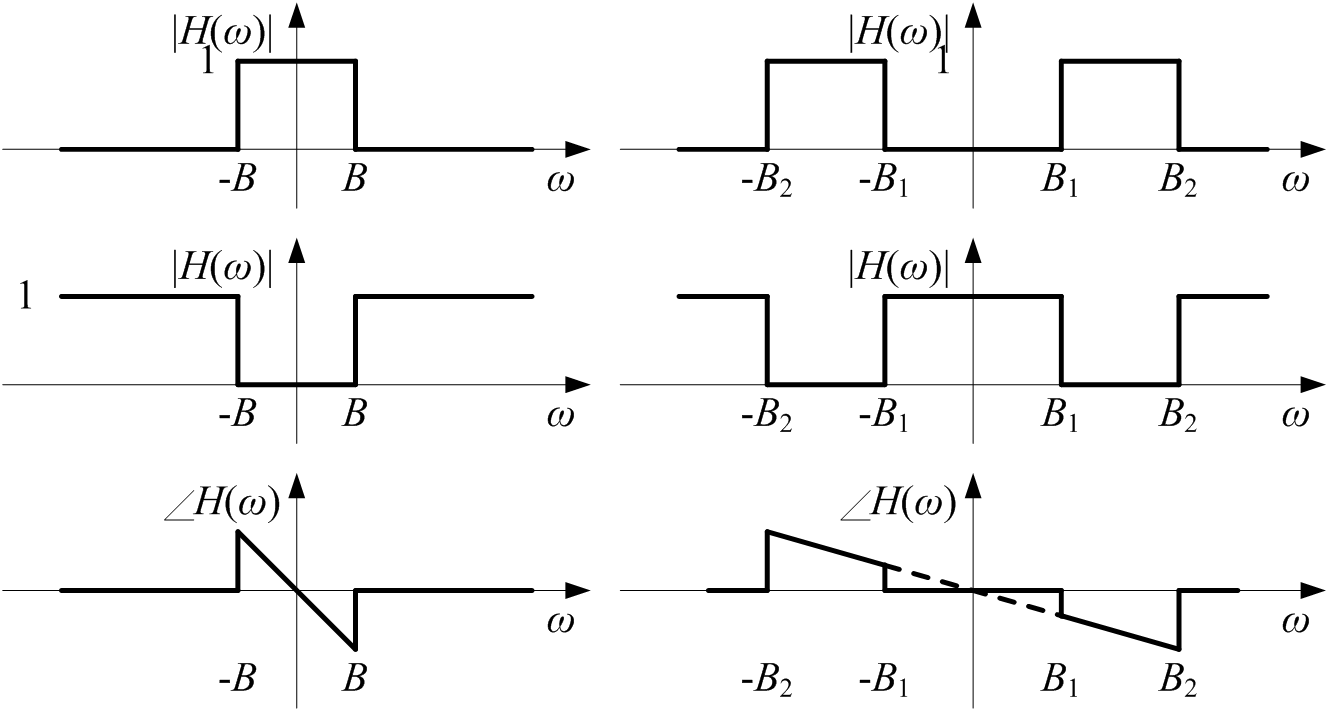
\includegraphics[height=6cm]{5.2.1-1.png}
\end{figure}

%============================================================
\subsection{理想低通滤波器的可能性}

理想的“全通”的频率响应应符合大小无衰减且相位线性,于是有:
\begin{align*}
&\because \begin{cases}
	\left| H\left( \omega \right) \right|=1\\
	\angle H\left( \omega \right) =-a\omega\\
\end{cases} \\
&\therefore H\left( \omega \right) =e^{ia\omega}
\end{align*}
则理想低通相当于全通被方波函数包络:
\[
H\left( \omega \right) =p_{2B}\left( \omega \right) \cdot e^{ia\omega}
\]
这是理想低通的频率响应。
根据傅里叶变换性质,系统的冲激响应:
\[
h\left( t \right) =\frac{B}{\pi}\mathrm{sinc}\frac{B\left( t-a \right)}{\pi}
\]
\begin{itemize}
    \item $B$:系统带宽;
    \item $a$:系统延时。
\end{itemize}
由于冲激响应在$t<0$都会有值,相当于作为输入的冲激还没有进系统,系统就有输出。
这种系统违反了因果律,所以理想低通是不存在的。






\newpage
\section{Nyquist采样定理}

本节简单介绍Nyquist采样定理。

假设信号$x\left( t \right) $,以$T$周期采样,采样后信号记为$x_s\left( t \right) $,则有:
\[
x_s\left( t \right) =\sum_{n=-\infty}^{+\infty}{x\left( t \right) \delta \left( t-nT \right)}
\]
假设信号的傅里叶变换$X\left( \omega \right) $,则采样信号$x_s\left( t \right) $的傅里叶变换有:
\[
X\left( \omega \right) =\sum_{n=-\infty}^{+\infty}{\frac{1}{T}X\left( t-n\omega _s \right)}
\]
其中,$\omega _s=2\pi /T$称为{\bf 采样频率}。
若信号在频域的带宽$B$有限,且采样频率满足$\omega _s>2B$,则采样本身不会对信号有任何影响,而且采样后的信号可以通过低通进行完全恢复,这就是{\bf Nyquist采样定理}。

Nyquist采样定理的前提是信号是有限带宽信号。
但实际信号因为时域有限而导致频域无限,本身就不满足Nyquist定理的先决条件,所以无论采样频率多高,都会使信号的高频发生混叠。
通常的做法是先让信号通过一个低通去掉高频,再进行采样。






\newpage
\section{Python应用}

本章的一个重点是能够借助Python,在频域角度分析系统对某输入的作用和输出结果。

本节要点:
\begin{itemize}
    \item 掌握Python分析方法。
\end{itemize}

%============================================================
\subsection{分析方法}

通常有一类问题是已知一个系统,要分析它的对信号产生的作用。
借助Python,一般步骤如下:
\begin{enumerate}
    \item 推导系统频域响应$H\left( \omega \right) $;
    \item 求解信号的傅里叶变换$X\left( \omega \right) $;
    \item 推导输出的时域函数$y\left( t \right) =\mathscr{F} ^{-1}\left[ H\left( \omega \right) \cdot X\left( \omega \right) \right] $。
\end{enumerate}

%============================================================
\subsection{例——RC电路分析}

\begin{example}
如下RC电路,设电压源为输入,电容两端电压为输出,分析不同的RC值对输出的影响。
\begin{figure}[h]
\centering
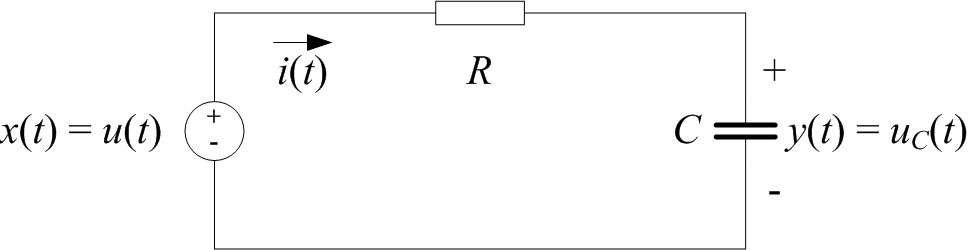
\includegraphics[height=2cm]{1.5.1-1.png}
\end{figure}
\[
x\left( t \right) =p_{\tau =1}\left( t \right) =\begin{cases}
	1,t\in \left[ -0.5,0.5 \right]\\
	0,t\notin \left[ -0.5,0.5 \right]\\
\end{cases}
\]
\end{example}

首先推导系统的频率响应,过程略:
\[
H\left( \omega \right) =\frac{1}{1+i\omega RC}
\]
分别取$RC=1,RC=0.1,RC=0.001$,系统频率响应的频谱图如下。
可见,减小电阻或电容都可以提高系统对高频的响应,特别在$RC=0.001$时,幅频图上看输出几乎没有衰减,相频图上看输出几乎没有相移。

\begin{python}
w  = np.arange(-50, 50, 0.01)
RC = 1;     H1 = 1 / (1 + RC * w * 1.0j)
RC = 0.1;   H2 = 1 / (1 + RC * w * 1.0j)
RC = 0.001; H3 = 1 / (1 + RC * w * 1.0j)

plot_mag_phs(w, np.abs(H1), np.angle(H1, deg=True),
             axs[0][0], axs[1][0], title=r"$H(\omega) ,RC=1$",     ...)
plot_mag_phs(w, np.abs(H2), np.angle(H2, deg=True),
             axs[0][1], axs[1][1], title=r"$H(\omega) ,RC=0.1$",   ...)
plot_mag_phs(w, np.abs(H3), np.angle(H3, deg=True),
             axs[0][2], axs[1][2], title=r"$H(\omega) ,RC=0.001$", ...)
\end{python}

\begin{figure}[h]
\centering
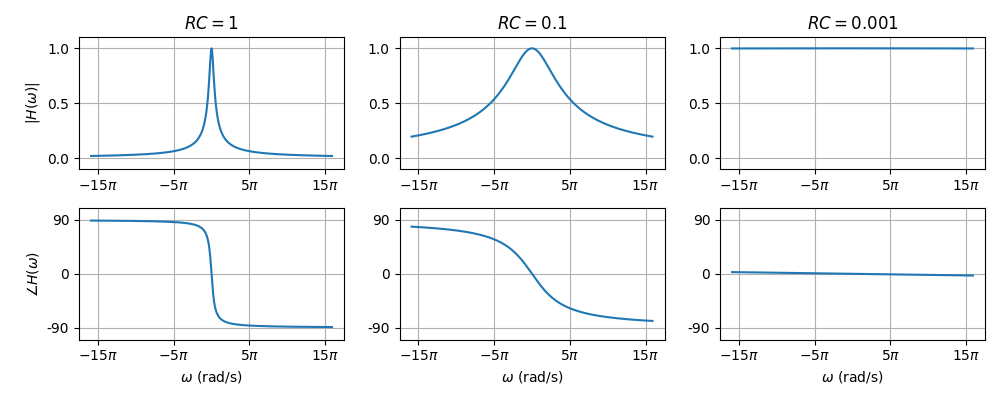
\includegraphics[height=4cm]{5.4.2-1.png}
\end{figure}

再分析输出信号的傅里叶变换,根据单方波的傅里叶变换计算输出的傅里叶:
\begin{align*}
&\because x\left( t \right) =p_{\tau =1}\left( t \right) \leftrightarrow X\left( \omega \right) =\frac{\sin \frac{\omega}{2}}{\frac{\omega}{2}} \\
&\therefore Y\left( \omega \right) =H\left( \omega \right) \cdot X\left( \omega \right) =\frac{1}{1+i\omega RC}\cdot \frac{\sin \frac{\omega}{2}}{\frac{\omega}{2}}
\end{align*}
取$RC=0.5,RC=0.001$,输入和输出的频谱图如下,$RC:0.5\rightarrow 0.001$提高了对输入信号高频部分的响应,使得输出更像输入。
\begin{figure}[h]
\centering
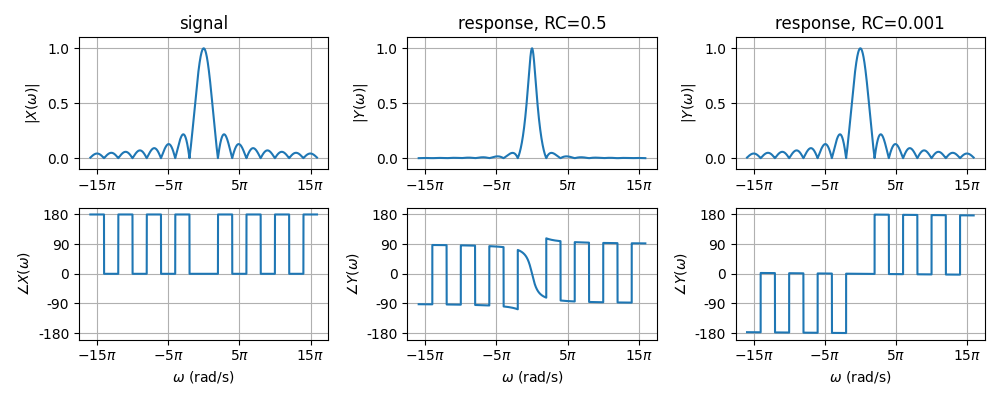
\includegraphics[height=4cm]{5.4.2-2.png}
\end{figure}

\begin{python}
w  = np.arange(-50, 50, 0.01)
X  = (np.sin(w/2) / (w/2))
RC = 0.5;   Y1 = 1 / (1 + RC * w * 1.0j) * (np.sin(w/2) / (w/2))
RC = 0.001; Y2 = 1 / (1 + RC * w * 1.0j) * (np.sin(w/2) / (w/2))

plot_mag_phs(w, np.abs(X),  np.angle(X, deg=True),
             axs[0][0], axs[1][0], title=r"$X(\omega)$",           ...)
plot_mag_phs(w, np.abs(Y1), np.angle(Y1, deg=True),
             axs[0][1], axs[1][1], title=r"$Y(\omega) ,RC=0.5$",   ...)
plot_mag_phs(w, np.abs(Y2), np.angle(Y2, deg=True),
             axs[0][2], axs[1][2], title=r"$Y(\omega) ,RC=0.001$", ...)
\end{python}










\chapter{离散傅里叶变换}

本章介绍离散傅里叶变换。
广义上,离散傅里叶变换分为“离散时间傅里叶变换(Discrete-Time Fourier Transform,DTFT)”和“离散的傅里叶变换(Discrete Fourier Transform,DFT)”。
前者是对离散时域信号的变换,得到的结果依然是连续频域,后者是对频域的离散。
由于数字处理的引入,DFT是离散傅里叶学习的最终目的。

本章要点:
\begin{itemize}
    \item 离散信号的傅里叶变换,DTFT。
    \item 离散傅里叶变换,DFT。
\end{itemize}

\begin{tcolorbox}
学习DTFT和DFT,特别要注意量纲和自变量的定义域。
\end{tcolorbox}

\newpage
\section{离散信号的傅里叶变换}

本节讨论离散信号的傅里叶变换(Discrete-Time Fourier Transform,DTFT)。
相应地,连续信号的傅里叶变换称为Continuous-Time Fourier Transform,CTFT。
本节是向离散傅里叶变换(Discrete Fourier Transform,DFT)的过渡。

本节要点:
\begin{itemize}
    \item 掌握DTFT;
    \item 熟悉CTFT和DTFT的关系;
    \item 理解采样周期对DTFT的影响。
\end{itemize}

%============================================================
\subsection{DTFT的概念}

\begin{definition}[离散信号的傅里叶变换]
我们已知连续信号$x\left( t \right) $的傅里叶变换
\begin{align*}
&X\left( \omega \right) =\int_{-\infty}^{+\infty}{x\left( t \right) e^{-i\omega t}dt} \\
&x\left( t \right) =\frac{1}{2\pi}\int_{-\infty}^{+\infty}{X\left( \omega \right) e^{i\omega t}d\omega}
\end{align*}
同样我们可以定义,若离散信号$x\left[ n \right] $满足:
\begin{itemize}
    \item 任一有限区域上满足狄利克雷收敛条件,
    \item 整个实数域绝对可积,即$\sum_{n=-\infty}^{+\infty}{\left| x\left[ n \right] \right|}$收敛,
\end{itemize}
则有:
\[
x\left[ n \right] =\frac{1}{2\pi}\int_0^{2\pi}{\left[ \sum_{n=-\infty}^{+\infty}{x\left[ n \right] e^{-i\varOmega n}} \right] e^{i\varOmega n}d\varOmega}
\]
同时称$\sum_{n=-\infty}^{+\infty}{x\left[ n \right] e^{-i\varOmega n}}$为{\bf 离散信号$x\left[ n \right] $的傅里叶变换}(Discrete-Time Fourier Transform,DTFT),记为$X\left( \varOmega \right) $,即:
\[
X\left( \varOmega \right) =\sum_{n=-\infty}^{+\infty}{x\left[ n \right] e^{-i\varOmega n}}
\]
相应地称
\[
x\left[ n \right] =\frac{1}{2\pi}\int_0^{2\pi}{X\left( \varOmega \right) e^{i\varOmega n}d\varOmega}
\]
为{\bf 离散信号的傅里叶逆变换}。离散信号的傅里叶变换形式通常记为:
\[
x\left[ n \right] \overset{\mathscr{F}}{\leftrightarrow}X\left( \varOmega \right)
\]
\end{definition}

\begin{tcolorbox}
注意,为区别连续信号,离散信号的傅里叶变换的自变量通常用大写$\varOmega $表示。
其次,$X\left( \varOmega \right) $依然是连续函数。
\end{tcolorbox}

%============================================================
\subsection{DTFT的量纲}

从定义看,信号的离散化使得$n$的量纲是时间,且有$\Delta n=n-\left( n-1 \right) =1$,于是:
\[
X\left( \varOmega \right) =\sum_{n=-\infty}^{+\infty}{\left\{ x\left[ n \right] e^{-i\varOmega n}\cdot \Delta n \right\}}
\]
易得$X\left( \varOmega \right) $的量纲依然是信号的量纲除以频率的量纲$\mathrm{D}_x\cdot \mathrm{Hz}^{-1}$,和CTFT一样。
这点从逆变换形式更好理解。

$\varOmega $的量纲和$\omega $一致,表示角频。
\begin{align*}
&\because \begin{cases}
	\omega \cdot t=s\\
	\varOmega \cdot n=\varOmega \cdot \frac{t}{T_{sample}}=s\\
\end{cases} \\
&\therefore \varOmega =\omega \cdot T_{sample}=\frac{\omega}{f_{sample}}
\end{align*}
其中$s$表示弧长。
可以认为$\varOmega $和$\omega $差了一个采样频率,相当于通过$T_{sample}$做了一个尺度变换。

%============================================================
\subsection{DTFT的极坐标形式}

DTFT可以变成极坐标形式:
\begin{align*}
X\left( \varOmega \right) &=\sum_{n=-\infty}^{+\infty}{x\left[ n \right] e^{-i\varOmega n}} \\
&=\sum_{n=-\infty}^{+\infty}{x\left[ n \right] \cos \left( n\varOmega \right)}+i\sum_{n=-\infty}^{+\infty}{-x\left[ n \right] \sin \left( n\varOmega \right)} \\
&=R\left( \varOmega \right) +iI\left( \varOmega \right)
\end{align*}
于是:
\begin{align*}
&\begin{cases}
	\left| X\left( \varOmega \right) \right|=\sqrt{R^2\left( \varOmega \right) +I^2\left( \varOmega \right)}\\
	\angle X\left( \varOmega \right) =\mathrm{arc}\tan \frac{I\left( \varOmega \right)}{R\left( \varOmega \right)}\\
\end{cases} \\
&X\left( \varOmega \right) =\left| X\left( \varOmega \right) \right|\cdot e^{i\angle X\left( \varOmega \right)}
\end{align*}
同样,DTFT的幅频是偶函数,相频是奇函数,且本身有$X\left( -\varOmega \right) =\bar{X}\left( \varOmega \right) $。

%============================================================
\subsection{广义DTFT}

对于有些函数,如$x\left[ n \right] =1$等,由于不满足绝对可积条件,没有严格意义上的DTFT,但可以通过单位冲激定义广义DTFT。

假设某信号DTFT之后有$2\pi \delta \left( \varOmega \right) $,则原信号:
\begin{align*}
&\because \frac{1}{2\pi}\int_{-\pi}^{+\pi}{2\pi \delta \left( \varOmega \right) e^{i\varOmega n}d\varOmega}=\int_{-\pi}^{+\pi}{\delta \left( \varOmega \right) e^{i\varOmega n}d\varOmega}=1 \\
&\therefore 1\overset{\mathscr{F}}{\rightarrow}2\pi \delta \left( \varOmega \right)
\end{align*}
以上只是一个例子,通过$\delta \left[ n \right] $的DTFT和DTFT的性质,我们可以求得很多函数的广义DTFT。

%============================================================
\subsection{DTFT的性质}

{\bf 奇偶性}

通过DTFT的直角坐标形式易得,如果$x\left[ n \right] $是偶函数,则其DTFT是实函数,如果$x\left[ n \right] $是奇函数,则其DTFT是纯虚函数,此外,一般DTFT是$\varOmega $的复变函数。
\begin{align*}
&x\left[ n \right] \text{ is even} \quad \Rightarrow \quad X\left( \varOmega \right) =x\left[ 0 \right] +2\sum_{n=1}^{+\infty}{x\left[ n \right] \cos \left( n\varOmega \right)} \\
&x\left[ n \right] \text{ is even} \quad \Rightarrow \quad X\left( \varOmega \right) =-2i\sum_{n=1}^{+\infty}{x\left[ n \right] \sin \left( n\varOmega \right)}
\end{align*}

{\bf 周期性}

对于任何离散信号,其DTFT都是周期函数,且$T=2\pi $。
简单证明:
\begin{align*}
X\left( \varOmega +2\pi \right) &=\sum_{n=-\infty}^{+\infty}{x\left[ n \right] e^{-i\left( \varOmega +2\pi \right) n}}=\sum_{n=-\infty}^{+\infty}{x\left[ n \right] e^{-i\varOmega n}e^{-i2\pi n}} \\
&=\sum_{n=-\infty}^{+\infty}{x\left[ n \right] e^{-i\varOmega n}}
\end{align*}
可见,DTFT的周期性源于信号的离散性。
由于$X\left( \varOmega \right) $的周期性,逆变换的积分范围可以是$\left[ 0,2\pi \right] $,也可以是$\left[ -\pi ,\pi \right] $。
加之DTFT的幅频是偶函数、相频是奇函数,所以DTFT的好处是对于信号的频域分析,只需要考察$\left[ 0,\pi \right] $即可。

{\bf 采样的频域特性}

\[
\begin{cases}
	x\left[ n \right] \leftrightarrow X\left( \varOmega \right)\\
	\gamma \left( t \right) \leftrightarrow X\left( \omega \right) p_{2\pi}\left( \omega \right)\\
\end{cases} \quad \Rightarrow \quad x\left[ n \right] =\left. \gamma \left( t \right) \right|_{t=n}=\gamma \left[ n \right]
\]

这说明所谓的采样,在频域看来就是通过一个带宽$B=\pi $的低通。
或者说,采样后信号的频域从原来的整个实数限制到$\left[ -\pi ,\pi \right] $。
简单证明:
\begin{align*}
&\because \gamma \left( t \right) =\frac{1}{2\pi}\int_{-\infty}^{+\infty}{X\left( \omega \right) p_{2\pi}\left( \omega \right) e^{i\omega t}d\omega}=\frac{1}{2\pi}\int_{-\pi}^{+\pi}{X\left( \omega \right) e^{i\omega t}d\omega} \\
&\therefore \gamma \left( n \right) =\frac{1}{2\pi}\int_{-\pi}^{+\pi}{X\left( \omega \right) e^{i\omega n}d\omega}=\frac{1}{2\pi}\int_{-\pi}^{+\pi}{X\left( \varOmega \right) e^{i\varOmega n}d\varOmega}=x\left[ n \right]
\end{align*}
上述证明过程中,$t$到$n$只是一个简单的变量替换,所以,这里的“采样”固定了周期$T=1$。
如果要获得不一样的采样周期,可以先在时域做尺度变换。

{\bf 线性性}

\[
ax\left[ n \right] +by\left[ n \right] \leftrightarrow aX\left( \varOmega \right) +bY\left( \varOmega \right)
\]

{\bf 时移性、频移性}

\begin{align*}
&x\left[ n-n_1 \right] \leftrightarrow X\left( \varOmega \right) \cdot e^{-i\varOmega n_1} \\
&e^{-i\varOmega _1n}\cdot x\left[ n \right] \leftrightarrow X\left( \varOmega -\varOmega _1 \right)
\end{align*}

{\bf 反转性}

\[
x\left[ -n \right] \leftrightarrow X\left( -\varOmega \right) =\bar{X}\left( \varOmega \right)
\]

注意,DTFT没有CTFT中的“时展性”。
或者说,DTFT的“时展性”体现在对连续信号的采样周期上。
采样周期确实对DTFT结果有影响。

{\bf 三角律}

\begin{align*}
&x\left[ n \right] \cos \varOmega _1t\leftrightarrow \frac{1}{2}\left[ X\left( \varOmega +\varOmega _1 \right) +X\left( \varOmega -\varOmega _1 \right) \right] \\
&x\left[ n \right] \sin \varOmega _1t\leftrightarrow \frac{i}{2}\left[ X\left( \varOmega +\varOmega _1 \right) -X\left( \varOmega -\varOmega _1 \right) \right]
\end{align*}

{\bf 时域和}

\[
\sum_{k=1}^n{x\left[ k \right]}\leftrightarrow \frac{1}{1-e^{-i\varOmega}}X\left( \varOmega \right) +\sum_{k=-\infty}^{+\infty}{\pi X\left( 2\pi k \right) \delta \left( \pi -2\pi k \right)}
\]

{\bf 频域的微分}

\[
\left( \frac{n}{i} \right) ^m\cdot x\left[ n \right] \leftrightarrow \frac{d^mX\left( \varOmega \right)}{d\varOmega ^m}
\]

{\bf 卷积性}

\begin{align*}
&x\left[ n \right] \ast y\left[ n \right] \leftrightarrow X\left( \varOmega \right) \cdot Y\left( \varOmega \right) \\
&x\left[ n \right] \cdot y\left[ n \right] \leftrightarrow \frac{1}{2\pi}\int_{-\pi}^{+\pi}{X\left( \varOmega -\lambda \right) Y\left( \lambda \right) d\lambda}
\end{align*}

{\bf Parseval定理}

\begin{align*}
&\sum_{n=-\infty}^{+\infty}{x\left[ n \right] y\left[ n \right]}=\frac{1}{2\pi}\int_{-\pi}^{+\pi}{\bar{X}\left( \varOmega \right) Y\left( \varOmega \right) d\varOmega} \\
&\sum_{n=-\infty}^{+\infty}{x^2\left[ n \right]}=\frac{1}{2\pi}\int_{-\pi}^{+\pi}{\left| X\left( \varOmega \right) \right|^2d\varOmega}
\end{align*}

\begin{tcolorbox}
注意,DTFT没有CTFT中的“Duality”。
\end{tcolorbox}

%============================================================
\subsection{CTFT和DTFT对比}

\begin{table}[h]
\centering
% \caption{表头}
\begin{tabular}{ccc}
    \toprule
    & CTFT & DTFT\\
    \midrule
    变换 & $X\left( \omega \right) =\int_{-\infty}^{+\infty}{x\left( t \right) e^{-i\omega t}dt}$ & $X\left( \varOmega \right) =\sum_{n=-\infty}^{+\infty}{x\left[ n \right] e^{-i\varOmega n}}$\\
    逆变换 & $x\left( t \right) =\frac{1}{2\pi}\int_{-\infty}^{+\infty}{X\left( \omega \right) e^{i\omega t}d\omega}$ & $x\left[ n \right] =\frac{1}{2\pi}\int_0^{2\pi}{X\left( \varOmega \right) e^{i\varOmega n}d\varOmega}$\\
    时域变量 & 连续时间$t$ & 离散时间$n$\\
    频域变量 & 连续频率$\omega $ & 连续频率$\varOmega \in \left[ -\pi ,\pi \right] $\\
    周期 & 无 & $T=2\pi $\\
    \bottomrule
\end{tabular}
\end{table}

%============================================================
\subsection{例}

\begin{example}
设两个信号$x\left( t \right) =0.5^tu\left( t \right) ,x\left[ n \right] =0.5^nu\left[ n \right] $,分析两者的傅里叶变换。
\end{example}

$x\left( t \right) =0.5^tu\left( t \right) $的CTFT:
\begin{align*}
X\left( \omega \right) &=\int_{-\infty}^{+\infty}{0.5^tu\left( t \right) e^{-i\omega t}dt}=\int_0^{+\infty}{\left( 0.5e^{-i\omega} \right) ^tdt} \\
&=\left. \frac{\left( 0.5e^{-i\omega} \right) ^t}{\ln \left( 0.5e^{-i\omega} \right)} \right|_{0}^{+\infty}=-\frac{1}{\ln \left( 0.5e^{-i\omega} \right)}=-\frac{1}{\ln 0.5-i\omega}
\end{align*}

$x\left[ n \right] =0.5^nu\left[ n \right] $的DTFT,为公比$\left| 0.5e^{-i\varOmega} \right|<1$的无穷等比数列的和:
\[
X\left( \varOmega \right) =\sum_{n=-\infty}^{+\infty}{x\left[ n \right] e^{-i\varOmega n}}=\sum_{n=-\infty}^{+\infty}{0.5^ne^{-i\varOmega n}}=\frac{1}{1-0.5e^{-i\varOmega}}
\]

\begin{python}
t   = np.arange(0, 5, 0.01)
x_t = 0.5**t
w   = np.arange(-3*np.pi, 3*np.pi, 0.01)
X_w = -1 / (np.log(0.5) - w*1.0j)
n   = np.arange(0,26)
x_n = 0.5**(0.2*n)
W   = np.arange(-3*np.pi, 3*np.pi, 0.01)
X_W = 1 / (1 - 0.5*np.exp(-1.0j*W))

axs[0][0].plot(t, x_t)
plot_mag_phs(w, np.abs(X_w), np.angle(X_w, deg=True), ...)
axs[0][1].stem(n, x_n)
plot_mag_phs(w, np.abs(X_W), np.angle(X_W, deg=True), ...)
\end{python}

\begin{figure}[h]
\centering
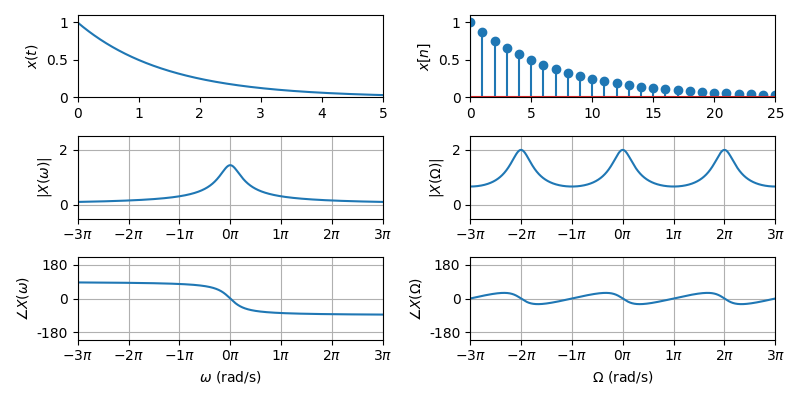
\includegraphics[height=5cm]{6.1.7-1.png}
\end{figure}

~

\begin{example}
设两个信号$x\left( t \right) =\left( -0.5 \right) ^tu\left( t \right) ,x\left[ n \right] =\left( -0.5 \right) ^nu\left[ n \right] $,(基本同上例,只是系数变成了-0.5,增强了信号波动频率),分析两者的傅里叶变换。
\end{example}

两个信号的傅里叶变换:
\begin{align*}
&\left( -0.5 \right) ^tu\left( t \right) \leftrightarrow -\frac{1}{\ln \left( -0.5 \right) -i\omega} \\
&\left( -0.5 \right) ^nu\left[ n \right] \leftrightarrow \frac{1}{1+0.5e^{-i\varOmega}}
\end{align*}

\begin{python}
t   = np.arange(0, 5, 0.01, dtype=np.complex64)
x_t = (-0.5)**t
w   = np.arange(-3*np.pi, 3*np.pi, 0.01)
X_w = -1 / (np.log(-0.5+0.0j) - 1.0j*w)
n   = np.arange(0,26, dtype=np.complex64)
x_n = (-0.5)**(0.2*n)
W   = np.arange(-3*np.pi, 3*np.pi, 0.01)
X_W = 1 / (1 + 0.5*np.exp(-1.0j*W))

axs[0][0].plot(t.real, x_t.real)
plot_mag_phs(w, np.abs(X_w), np.angle(X_w, deg=True), ...)
axs[0][1].stem(n.real, x_n.real)
plot_mag_phs(w, np.abs(X_W), np.angle(X_W, deg=True), ...)
\end{python}

\begin{figure}[h]
\centering
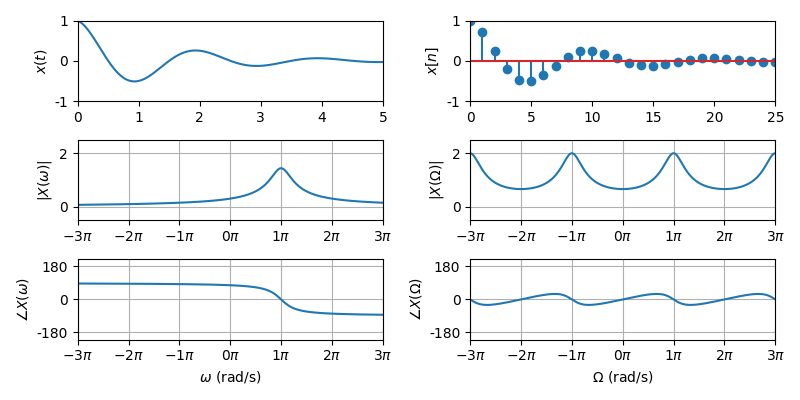
\includegraphics[height=5cm]{6.1.7-2.png}
\end{figure}

\begin{itemize}
    \item DTFT依然呈现周期性;
    \item 对比两个FT,0.5的FT集中在低频,-0.5的FT集中在高频。
\end{itemize}

%============================================================
\subsection{采样周期对DTFT的影响}

从量纲分析可得,DTFT和CTFT两者的意义相同,区别只在于变量。
由于对时域信号做了采样,所以暂时可以认为$\varOmega $对于$\omega $做了尺度变换,$\varOmega =\omega \cdot T_{sample}$。
而且通常$T_{sample}<1$,相当于信号变慢。
所以随着采样频率的提高,DTFT结果会向低频段集中。

实际上,DTFT的频率范围只是$\left[ -\pi ,\pi \right] $,其他部分都是周期性的复现。
由于对称性,实际分析的只是$\left[ 0,\pi \right] $,称为“窗口”。
DTFT在频率轴上开了一个窗口,将CTFT的频率“映射”到$\left[ 0,\pi \right] $,通过采样频率将CTFT的$0\text{~}\pi \cdot f_{sample}$部分映射到窗口中。
所以采样频率越高,我们在DTFT上看到的频率越宽广。

用前面的例子说明。
假设时域信号$x\left( t \right) =\left( -0.5 \right) ^t\cdot u\left( t \right) $,分析采样周期$T$对DTFT的影响。

令$t=nT$进行离散化,得到DTFT结果:
\begin{align*}
x\left[ n \right] &=\left( -0.5 \right) ^{nT}=\left[ \left( -0.5 \right) ^T \right] ^n \\
X\left( \varOmega \right) &=\sum_{n=-\infty}^{+\infty}{x\left[ n \right] e^{-i\varOmega n}}=\sum_{n=-\infty}^{+\infty}{\left[ \left( -0.5 \right) ^T \right] ^ne^{-i\varOmega n}} \\
&=\frac{1}{1-\left( -0.5 \right) ^Te^{-i\varOmega}}
\end{align*}
\begin{figure}[h]
\centering
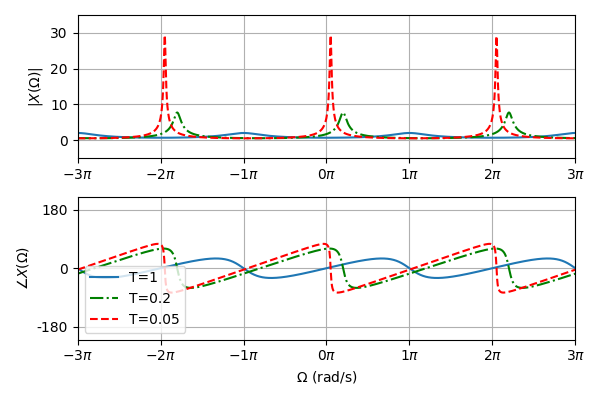
\includegraphics[height=5cm]{6.1.8-1.png}
\end{figure}

\begin{python}
W = np.arange(-3*np.pi, 3*np.pi, 0.01)
T = 1;    X_1 = 1 / (1 - (-0.5)**T * np.exp(-1.0j*W))
T = 0.2;  X_2 = 1 / (1 - (-0.5)**T * np.exp(-1.0j*W))
T = 0.05; X_3 = 1 / (1 - (-0.5)**T * np.exp(-1.0j*W))

plot_mag_phs(W, np.abs(X_1), np.angle(X_1, deg=True),
             mag_line_fmt='-', phs_line_fmt='-',
             mag_line_label='T=1', phs_line_label='T=1')
plot_mag_phs(W, np.abs(X_2), np.angle(X_2, deg=True),
             mag_line_fmt='g-.', phs_line_fmt='g-.',
             mag_line_label='T=0.2', phs_line_label='T=0.2')
plot_mag_phs(W, np.abs(X_3), np.angle(X_3, deg=True),
             mag_line_fmt='r--', phs_line_fmt='r--',
             mag_line_label='T=0.05', phs_line_label='T=0.05')
\end{python}

注意:
\begin{itemize}
    \item $T=1$时,可以认为就是原信号,即$X\left( \varOmega \right) =X\left( \omega \right) $。
    \item 随着采样频率的提高,DTFT窗口看到的频率越宽,使得“峰越往低频方向偏移”,或者认为在同样的 的“步频”下,采样频率越高信号“走得越慢”。
\end{itemize}






\newpage
\section{基于DTFT的系统频域分析}

本节在频域角度,讨论离散系统的响应。

本节要点:
\begin{itemize}
    \item 离散系统频率响应的概念;
    \item 了解采样频率对输出的影响。
\end{itemize}

%============================================================
\subsection{离散系统的频域响应定理}

\begin{theorem}[离散系统的频域响应定理]
如果一个零状态LTI系统满足绝对稳定的条件,即$\sum_{n=-\infty}^{+\infty}{\left| h\left[ n \right] \right|}<\infty $,则系统对于任意非周期信号$x\left[ n \right] $在时域的输出可以表示为卷积:
\[
y\left[ n \right] =x\left[ n \right] \ast h\left[ n \right]
\]
在频域的输出可以表示为DTFT的乘积:
\[
Y\left( \varOmega \right) =X\left( \varOmega \right) \cdot H\left( \varOmega \right)
\]
\begin{itemize}
    \item $x\left[ n \right] ,y\left[ n \right] $:输入输出信号的时域表达式;
    \item $h\left[ n \right] $:系统的冲激响应;
    \item $X\left( \varOmega \right) ,Y\left( \varOmega \right) $:输入输出信号的DTFT;
    \item $H\left( \varOmega \right) $:{\bf 离散系统的频率响应函数}(frequency response function),或称{\bf 系统函数}(system function),即$h\left[ n \right] $的傅里叶变换。
\end{itemize}
\end{theorem}

一个满足绝对稳定条件的LTI系统对任何输入的信号,系统会单独作用其各个频率分量的幅度和相位:
\begin{align*}
&\left| Y\left( \varOmega \right) \right|=\left| X\left( \varOmega \right) \right|\cdot \left| H\left( \varOmega \right) \right| \\
&\angle Y\left( \varOmega \right) =\angle X\left( \varOmega \right) +\angle H\left( \varOmega \right)
\end{align*}

%============================================================
\subsection{理想低通和采样频率对信号的影响}

数字系统对时域信号通常的做法是先采样进行离散化,再通过一个数字滤波器。
这里考察数字滤波器(即系统本身)和采样过程对信号通过性的影响。

首先考察滤波器对信号的输出结果。
由于DTFT的周期性,离散系统的频率响应函数是一个$T=2\pi $的周期函数。
假设一LTI离散系统(理想低通)有如下频率响应函数:
\begin{figure}[ht]
\centering
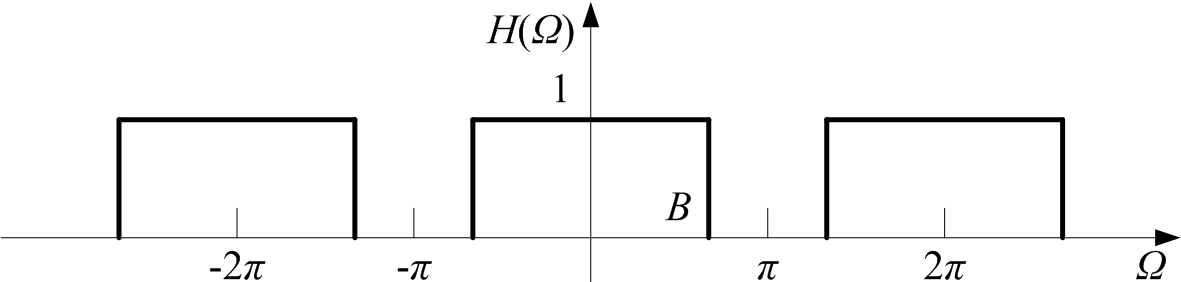
\includegraphics[height=2.5cm]{6.2.2-1.png}
\end{figure}
\[
H\left( \varOmega \right) =\sum_{n=-\infty}^{+\infty}{p_{2B}\left( \varOmega +2\pi n \right)}
\]

对比CTFT的系统频域分析,这里要注意几点:
\begin{itemize}
    \item 由于DTFT的周期性,一般考察区间$\left[ -\pi ,\pi \right] $,往0方向的是低频,往$\pm \pi $方向的是高频。
    \item 由于的频谱的对称性,考察区间可缩小为$\left[ 0,\pi \right] $。
\end{itemize}

\begin{tcolorbox}
这样的理想低通是不存在的,因为其冲激响应$h\left[ n \right] =\frac{B}{\pi}\sin\mathrm{c}\left( \frac{B}{\pi}n \right) $不符合因果性。
\end{tcolorbox}

对于简单的正弦信号$x\left[ n \right] =A\cos \left( \varOmega _0n \right) $,其DTFT有
\[
X\left( \varOmega \right) =\sum_{m=-\infty}^{\infty}{A\pi \left[ \delta \left( \varOmega +\varOmega \,\,_0+2\pi m \right) +\delta \left( \varOmega -\varOmega \,\,_0+2\pi m \right) \right]}
\]
只要$\varOmega _0\leqslant B$,信号就能通过该系统,如下图。
\begin{figure}[h]
\centering
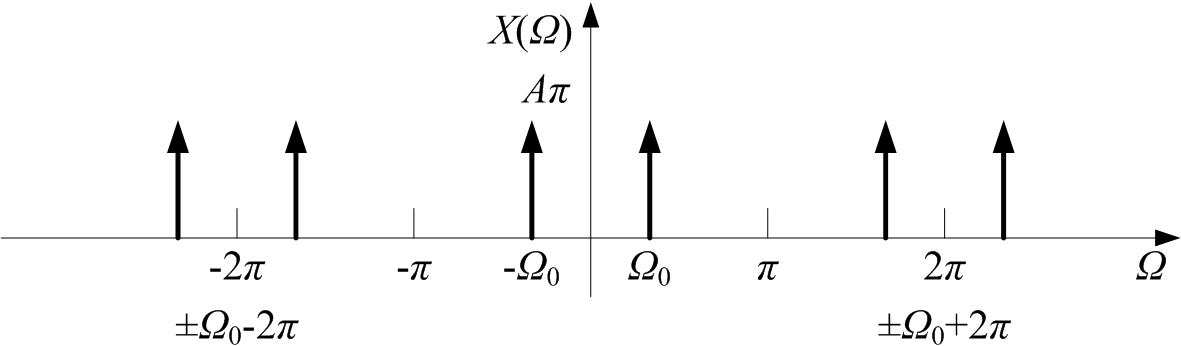
\includegraphics[height=3cm]{6.2.2-2.png}
\end{figure}

再考察采样对输出的影响。
假设连续时域信号$x\left( t \right) =A\cos \left( \omega _0t \right) $,对其采样
\begin{align*}
&x\left[ n \right] =\left. x\left( t \right) \right|_{t=nT}=A\cos \left( \omega _0nT \right) \overset{\varOmega _0=\omega _0T}{=}A\cos \left( \varOmega _0n \right) \\
&n=0,\pm 1,\pm 2,\cdots
\end{align*}
要使$\varOmega _0\leqslant B$,即$\omega _0T\leqslant B$,也即$T\leqslant B/\omega _0$。

\begin{tcolorbox}
采样频率越高,DTFT映射到的实际频率范围越宽。
\end{tcolorbox}

%============================================================
\subsection{均值滤波器}

考虑最简单的平均化,系统的输入输出差分方程为:
\[
y\left[ n \right] =\frac{1}{N}\sum_{k=0}^{N-1}{x\left[ n-k \right]}
\]
一般认为当$N\geqslant 3$时有较为锋利的截止,这样的系统称为{\bf 均值滤波器}(mean filter),频率响应函数:
\begin{align*}
&\because h\left[ n \right] =\frac{1}{N}\sum_{k=0}^{N-1}{\delta \left[ n-k \right]} \\
&\because \begin{cases}
	x\left[ n-n_1 \right] \leftrightarrow X\left( \varOmega \right) \cdot e^{-i\varOmega n_1}\\
	\delta \left[ n \right] \leftrightarrow 1\\
\end{cases} \\
&\therefore H\left( \varOmega \right) =\frac{1}{N}\sum_{k=0}^{N-1}{e^{-i\varOmega k}}
\end{align*}

\begin{python}
def mean_filter(N, W):
	H = 1
	for i in range(1, N):
		H = H + np.exp(-1.0j * i * W)
		pass
	H = H / N
	return H

W  = np.arange(-3*np.pi, 3*np.pi, 0.01)
N1 = 2;  H1 = mean_filter(N1, W)
N2 = 5 ; H2 = mean_filter(N2, W)
N3 = 20; H3 = mean_filter(N3, W)

plot_mag_phs(W, np.abs(H1), np.angle(H1, deg=True), ...)
plot_mag_phs(W, np.abs(H2), np.angle(H2, deg=True), ...)
plot_mag_phs(W, np.abs(H3), np.angle(H3, deg=True), ...)
\end{python}

\begin{figure}[h]
\centering
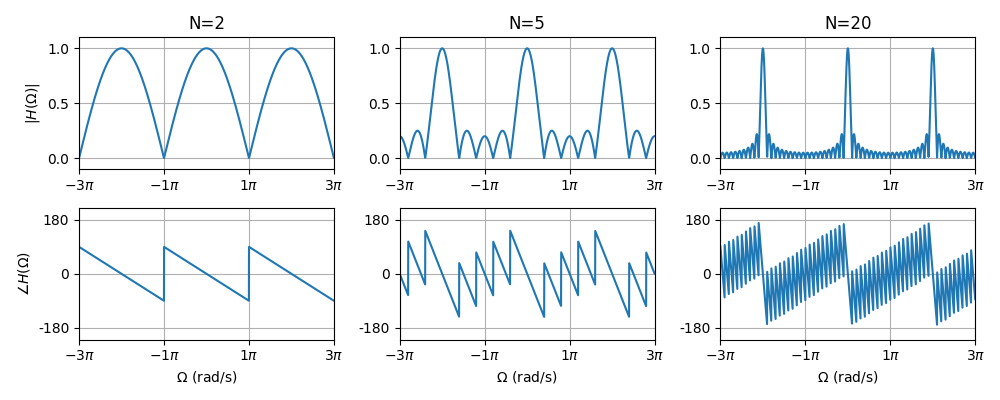
\includegraphics[height=4cm]{6.2.3-1.png}
\end{figure}

由幅频图可得系统是个低通,且阶数越高带宽越小,时域上就是抹得越平。






\newpage
\section{离散傅里叶变换}

之前的章节,从CTFT到DTFT,完成了从连续信号到离散信号的傅里叶分析。
\[
\begin{cases}
	X\left( \omega \right) =\int_{-\infty}^{+\infty}{x\left( t \right) e^{-i\omega t}dt}\\
	x\left( t \right) =\frac{1}{2\pi}\int_{-\infty}^{+\infty}{X\left( \omega \right) e^{i\omega t}d\omega}\\
\end{cases}\,\,  \Rightarrow \,\,  \begin{cases}
	X\left( \varOmega \right) =\sum_{n=-\infty}^{+\infty}{x\left[ n \right] e^{-i\varOmega n}}\\
	x\left[ n \right] =\frac{1}{2\pi}\int_{-\infty}^{+\infty}{X\left( \varOmega \right) e^{i\varOmega t}d\varOmega}\\
\end{cases}
\]
DTFT从非周期性的连续谱变成周期性的连续谱($0\text{~}2\pi $的稠密的连续谱)。
本节介绍对DTFT的离散化,获得一个离散的傅里叶变换结果。

本节要点:
\begin{itemize}
    \item 掌握DFT;
    \item 熟悉CTFT、DTFT和DFT三者关系;
    \item 掌握DFT的Python实现;
    \item 充分理解采样频率和采样数量对DFT的影响。
\end{itemize}

%============================================================
\subsection{DFT的概念}

\begin{definition}[离散傅里叶变换]
假设离散信号$x\left[ n \right] $只在$n\in \left[ 0,N \right) $上有定义(即$n=0,1,2,\cdots ,N-1$,一般$N$很大,如1024),则称:
\[
X\left[ m \right] =\sum_{n=0}^{N-1}{x\left[ n \right] e^{-i\left( \frac{2\pi}{N}m \right) n}} \qquad m=0,1,2,\cdots ,N-1
\]
为{\bf 离散信号$x\left[ n \right] $的离散傅里叶变换}(Discrete Fourier Transform,DFT)。
相应地称
\[
x\left[ n \right] =\frac{1}{N}\sum_{m=0}^{N-1}{X\left[ m \right] e^{i\left( \frac{2\pi}{N}n \right) m}} \qquad n=0,1,2,\cdots ,N-1
\]
为{\bf 离散傅里叶逆变换}(inverse Discrete Fourier Transform,iDFT)。
离散信号的傅里叶变换形式通常记为:
\[
x\left[ n \right] \overset{\mathscr{F}}{\leftrightarrow}X\left[ m \right]
\]
\end{definition}

由于DFT和iDFT都是有限和,所以离散傅里叶变换和逆变换总是存在的。其次,由于DFT的求和区间是$\left[ 0,N \right) $,所以DFT不是周期函数。

%============================================================
\subsection{DFT的量纲}

由于这里$N$的带有信号总时长的属性,可以认为有时间量纲,所以$X\left[ m \right] $的量纲依然是信号量纲除以频率($\mathrm{D}_x\cdot \mathrm{Hz}^{-1}$),表示单位频率的信号的量,即信号的频率密度。
如果考虑到$n,N$的时间量纲属性,$m$无量纲。
如果考虑到$t=n\cdot T_{sample}$,则有
\begin{align*}
&\because \begin{cases}
	\omega \cdot t=s\\
	\frac{2\pi}{N}\cdot m\cdot \frac{t}{T_{sample}}=s\\
\end{cases} \\
&\therefore \omega =\frac{2\pi}{N}\cdot m\cdot \frac{1}{T_{sample}}=\frac{\omega _{sample}}{N}\cdot m
\end{align*}
其中$s$表示弧长。
$m$依然无量纲。
但其物理意义很清楚,对于采样频率$N$等分之后的序数。
可令基频$\omega _0=\frac{\omega _{sample}}{N}$,则有$\omega =m\omega _0$。
$X\left[ m \right] $代表信号在频率$\frac{\omega _{sample}}{N}\cdot m$(或$\frac{f_{sample}}{N}\cdot m$)处的分量,且$m\in \left[ 0,N \right) $。

~

若采样频率1000Hz,采样100个数据$x\left[ 0 \right] \text{~}x\left[ 99 \right] $,DFT之后得到100个频域数据$X\left[ 0 \right] \text{~}X\left[ 99 \right] $。
由于对称性,只需要考察$X\left[ 0 \right] \text{~}X\left[ 49 \right] $。
$X\left[ 0 \right] $表示信号的直流分量,$X\left[ 1 \right] $表示信号$\frac{1000\mathrm{Hz}}{100}\cdot 1=10\mathrm{Hz}$的分量,以此类推,$X\left[ 49 \right] $表示信号$\frac{1000\mathrm{Hz}}{100}\cdot 49=490\mathrm{Hz}$的分量。
特别注意,由于对称性$X\left[ 99 \right] $表示信号10Hz的分量!

从上述分析可以得到:
\begin{itemize}
    \item 采样频率越高,越能看到信号的高频,即若要分析某信号位于$f_0$的分量,则采样频率至少需要其两倍$f_{sample}=2f_0$。
    \item 采样数据决定了频谱的分辨率,若频谱要看的细致,则必须采集更多的信号值。
\end{itemize}
即,采样频率决定了DFT的呈现范围,采样量决定了DFT的细腻程度。

%============================================================
\subsection{DFT的直角坐标形式}

DFT的直角坐标形式:
\begin{align*}
&X\left[ m \right] =\sum_{n=0}^{N-1}{x\left[ n \right] e^{-i\left( \frac{2\pi}{N}n \right) m}} \\
&=\sum_{n=0}^{N-1}{x\left[ n \right] \cos \left( \frac{2\pi n}{N}m \right)}+i\sum_{n=0}^{N-1}{-x\left[ n \right] \sin \left( \frac{2\pi n}{N}m \right)} \\
&\begin{cases}
	R\left[ m \right] =\sum_{n=0}^{N-1}{x\left[ n \right] \cos \left( \frac{2\pi n}{N}m \right)}=x\left[ 0 \right] +\sum_{n=1}^{N-1}{x\left[ n \right] \cos \frac{2\pi nm}{N}}\\
	I\left[ m \right] =\sum_{n=0}^{N-1}{-x\left[ n \right] \sin \left( \frac{2\pi n}{N}m \right)}=-\sum_{n=1}^{N-1}{x\left[ n \right] \sin \frac{2\pi nm}{N}}\\
\end{cases}
\end{align*}

由于DFT的求和区间是$\left[ 0,N \right) $,而非像DTFT一样区间关于原点对称,所以信号的奇偶性并不影响DFT的复变函数形式。

%============================================================
\subsection{Python应用——DFT和iDFT函数}

这里,我们编写两个Python函数(my\_dft和my\_idft)用以求解有限离散信号的DFT和iDFT:
\begin{align*}
&X\left[ m \right] =\sum_{n=0}^{N-1}{x\left[ n \right] e^{-i\left( \frac{2\pi}{N}m \right) n}} \qquad m=0,1,2,\cdots ,N-1 \\
&x\left[ n \right] =\frac{1}{N}\sum_{m=0}^{N-1}{X\left[ m \right] e^{i\left( \frac{2\pi}{N}n \right) m}} \qquad n=0,1,2,\cdots ,N-1
\end{align*}

\begin{python}
def my_dft(x:np.ndarray) -> np.ndarray:
    X = np.zeros_like(x, dtype=np.complex64)
    N = x.size
    n = np.arange(0, x.size)
    for m in range(0, x.size):
        X[m] = np.dot(x, np.exp(0-1.0j*2*np.pi*m*n/N))
    return X

def my_idft(X:np.ndarray) -> np.ndarray:
    x = np.zeros_like(X, dtype=np.float64)
    M = X.size
    m = np.arange(0, X.size)
    for n in range(0, X.size):
        x[n] = np.dot(X, np.exp(0+1.0j*2*np.pi*m*n/M)) / M
        pass
    return x
\end{python}

%============================================================
\subsection{CTFT、DTFT和DFT三者关系}

{\bf CTFT}

\begin{align*}
&X\left( \omega \right) =\int_{-\infty}^{+\infty}{x\left( t \right) e^{-i\omega t}dt} \qquad \omega \in \mathbb{R} \\
&x\left( t \right) =\frac{1}{2\pi}\int_{-\infty}^{+\infty}{X\left( \omega \right) e^{i\omega t}d\omega} \qquad t\in \mathbb{R}
\end{align*}

{\bf DTFT}

\begin{align*}
&X\left( \varOmega \right) =\sum_{n=-\infty}^{+\infty}{x\left[ n \right] e^{-i\varOmega n}} \qquad \varOmega \in \left[ 0,2\pi \right) \\
&x\left[ n \right] =\frac{1}{2\pi}\int_0^{2\pi}{X\left( \varOmega \right) e^{i\varOmega n}d\varOmega} \qquad n\in \mathbb{Z}
\end{align*}

{\bf DFT}

\begin{align*}
&X\left[ m \right] =\sum_{n=0}^{N-1}{x\left[ n \right] e^{-i\frac{2\pi mn}{N}}} \qquad m\in \left[ 0,N \right) \\
&x\left[ n \right] =\frac{1}{N}\sum_{m=0}^{N-1}{X\left[ m \right] e^{i\frac{2\pi nm}{N}}} \qquad n\in \left[ 0,N \right)
\end{align*}

进一步对比DTFT和DFT对频率的处理,假设$x\left[ n \right] $只在$n\in \left[ 0,N \right) $上有定义,则:
\begin{align*}
&X\left( \varOmega \right) =\sum_{n=-\infty}^{+\infty}{x\left[ n \right] e^{-i\varOmega n}}=\sum_{n=0}^{N-1}{x\left[ n \right] e^{-i\varOmega n}} \\
&X\left[ m \right] =\sum_{n=0}^{N-1}{x\left[ n \right] e^{-i\left( \frac{2\pi}{N}m \right) n}}
\end{align*}
两者差别在于DFT将DTFT的连续频域变量$\varOmega $离散化为$m$,或者说对频域进行了采样,间隔为$2\pi /N$,采样$N$个点:
\[
\varOmega \,\,=\frac{2\pi}{N}m \qquad m=0,1,2,\cdots ,N-1
\]

%============================================================
\subsection{采样频率和采样数量对DFT的影响}

\begin{figure}[h]
\centering
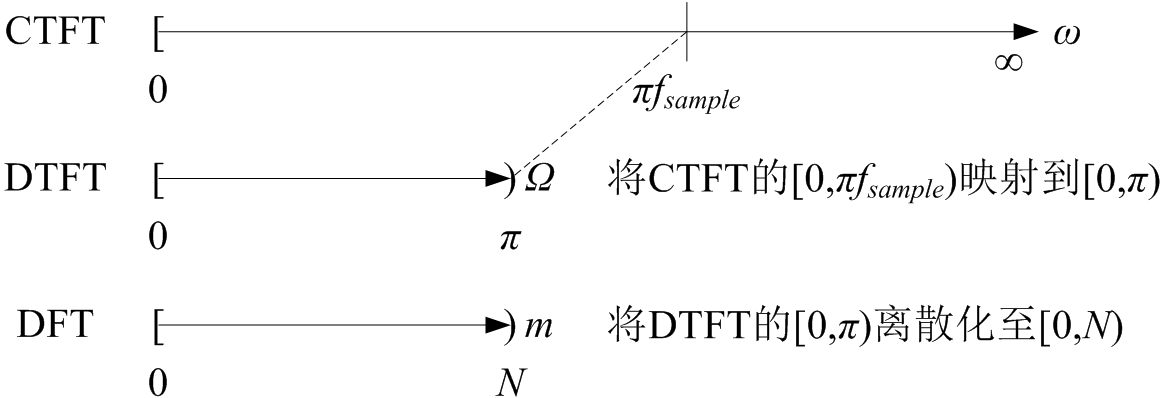
\includegraphics[height=3cm]{6.3.6-1.png}
\end{figure}

{\bf 采样频率$f_{sample}$的影响}

DTFT将CTFT的$0\text{~}\pi \cdot f_{sample}$部分映射到窗口$\left[ 0,\pi \right] $中,所以采样频率决定DTFT能看到多高频率范围,$f_{sample}$越高,越能收集信号的变化,对应地DTFT越能看到高频,越逼近CTFT。

{\bf 采样数量$N$的影响}

DFT再将DTFT的窗口离散化成$\left[ 0,N/2 \right) $,$X\left[ m \right] $的整体包络就是$X\left( \varOmega \right) $,所以信号序列的长度(即$N$)并不改变$X\left[ m \right] $的整体形状,$N$越大,表示对信号收集地越多,DFT越密集、分辨率越高、越细腻,越能精确描述包络形状,越贴近对应的$X\left( \varOmega \right) $曲线。

综合来讲,对于同样的信号,$f_{sample}$决定了你能看到多宽的频率(即频率的上限),$N$决定了你能看到多细腻的频谱,或者说DFT和CTFT的“长相一致程度”。

~

\begin{example}
假设有一个方波信号,前10秒是1,后面都是0,分析不同的采样数量和不同的采样频率对DFT的影响。
\end{example}

信号及其傅里叶变换如下图:
\begin{figure}[h]
\centering
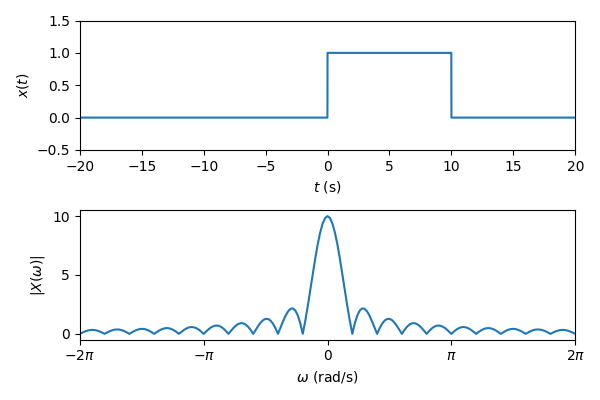
\includegraphics[height=4cm]{6.3.6-2.png}
\end{figure}

先分析不同的采样数量对DFT的影响,假设采样周期1s,即:
\[
x\left[ n \right] =1 \qquad n=0,1,2,3,4,5,6,7,8,9
\]
取三个不同的采样数量(10s,20s,110s),用Python计算DFT并作图:

\begin{python}
n_1  = np.arange(0, 10)
xn_1 = np.ones(10)
Xm_1 = my_dft(xn_1)

n_2  = np.arange(0, 20)
xn_2 = np.where(n_2<10, 1, 0)
Xm_2 = my_dft(xn_2)

n_3  = np.arange(0, 110)
xn_3 = np.where(n_3<10, 1, 0)
Xm_3 = my_dft(xn_3)

axs[0].stem(n_1, np.abs(Xm_1))
axs[1].stem(n_2, np.abs(Xm_2))
axs[2].stem(n_3, np.abs(Xm_3))
\end{python}

\begin{itemize}
    \item 如果采样数量小于等于方波,则这个序列其实可以认为是$x\left[ n \right] =1$,DFT也说明了这个问题;
    \item 采样数量越多,越能说明原连续信号,DFT的结果约贴近CTFT,结合量纲分析,就是频谱的分辨率更高。
\end{itemize}

\begin{figure}[ht]
\centering
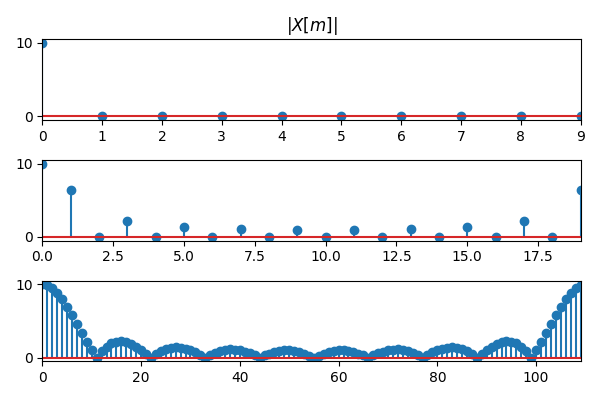
\includegraphics[height=5cm]{6.3.6-3.png}
\end{figure}

再分析采样频率对DFT的影响,分别用三种不同的采样频率(1s,0.5s,0.2s),采样数量都为50s,用Python计算DFT并作图:

\begin{python}
n_1  = np.arange(0, 50)
xn_1 = np.where(n_1<10, 1, 0)
Xm_1 = my_dft(xn_1)

n_2  = np.arange(0, 100)
xn_2 = np.where(n_2<20, 1, 0)
Xm_2 = my_dft(xn_2)

n_3  = np.arange(0, 250)
xn_3 = np.where(n_3<50, 1, 0)
Xm_3 = my_dft(xn_3)

axs[0].plot(n_1, np.abs(Xm_1))
axs[1].plot(n_2, np.abs(Xm_2))
axs[2].plot(n_3, np.abs(Xm_3))
\end{python}

\begin{figure}[h]
\centering
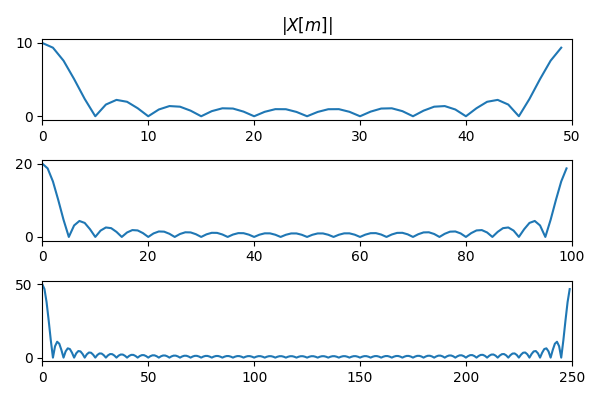
\includegraphics[height=5cm]{6.3.6-4.png}
\end{figure}

\begin{itemize}
    \item 为了看清,使用plot函数作图;
    \item 采样频率影响DFT的大致形状;
    \item 采样频率不影响lobe的“宽度”(即DFT两个相邻0值的间隔距离),影响lobe的“厚度”;
    \item 采样频率越高,频率范围越“拥挤”,即可看到的频率越多,结合量纲分析就是越能看到高频部分;
    \item 采样频率越高,DFT低频份量占比越多,这和采样周期对DTFT的影响的分析一致。
\end{itemize}

%============================================================
\subsection{填充技术对DFT的影响}

虽然采样数量越多,DFT越能体现CTFT,但真实系统对采样数量还是有要求的,采样数量不可能无限多。
这里讨论一种填充技术,书中称为“DFT of truncated signal”。

如下连续信号,以$T=0.5$采样,信号及其傅里叶变换如下:
\begin{align*}
&x\left( t \right) =0.9^t \qquad t\geqslant 0 \\
&X\left( \omega \right) =-\frac{1}{\ln 0.9-i\omega}
\end{align*}
\begin{figure}[h]
\centering
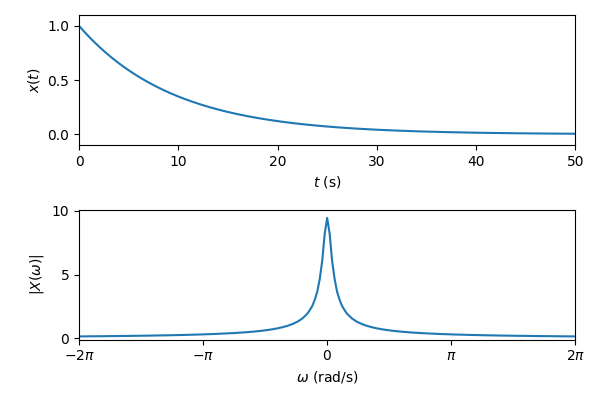
\includegraphics[height=4cm]{6.3.7-1.png}
\end{figure}
% \begin{figure}[h]
% \centering
%     \begin{minipage}{0.48\linewidth}
%     \centerline{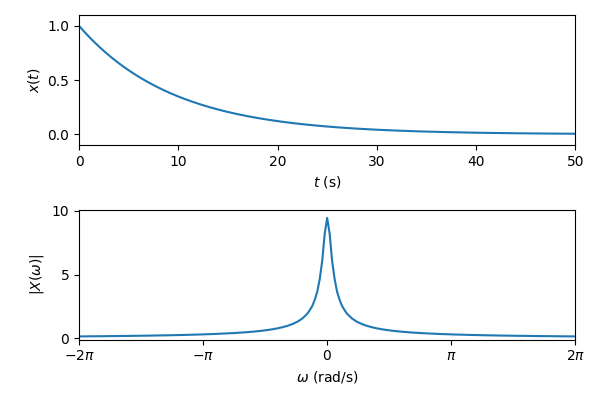
\includegraphics[height=4cm]{6.3.7-1.png}}
%     \end{minipage}
% \hfill
%     \begin{minipage}{0.48\linewidth}
%     \begin{align*}
%     &x\left( t \right) =0.9^t \qquad t\geqslant 0 \\
%     &X\left( \omega \right) =-\frac{1}{\ln 0.9-i\omega}
%     \end{align*}
%     \end{minipage}
% \end{figure}

使用Python辅助分析:
\begin{python}
n_1  = np.arange(0, 30, 0.5)
xn_1 = 0.9**n_1
Xm_1 = my_dft(xn_1)

n_2  = np.arange(0, 10, 0.5)
xn_2 = 0.9**n_2
Xm_2 = my_dft(xn_2)

n_3  = np.arange(0, 30, 0.5)
xn_3 = 0.9**n_3; xn_3[xn_2.size:] = 0
Xm_3 = my_dft(xn_3)

axs[0].plot(np.abs(Xm_1))
axs[1].plot(np.abs(Xm_2))
axs[2].plot(np.abs(Xm_3))
\end{python}

\begin{itemize}
    \item 足额采样,xn\_1采样前30s,DFT结果Xm\_1大致能体现CTFT,如下第一幅;
    \item 采样不足,xn\_2只采样前10s,DFT结果Xm\_2开始有明显失真,如下第二幅。
    \item 填充技术弥补采样不足,xn\_2只采样前10s,后20s人为填充0,相当于时域叠加了方波,DFT结果Xm\_3叠加了sinc函数,如下第三幅。
\end{itemize}

\begin{figure}[h]
\centering
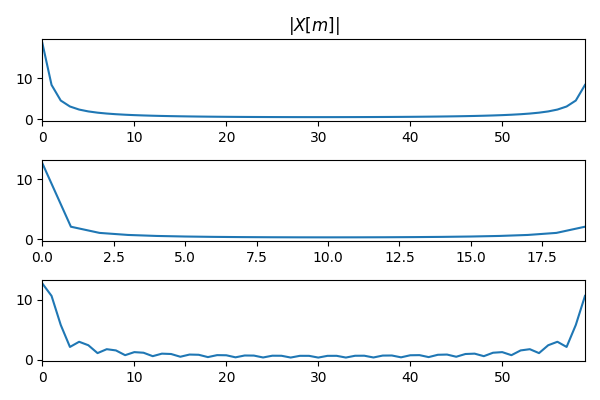
\includegraphics[height=5cm]{6.3.7-2.png}
\end{figure}

填充技术其实是一种“伪细腻化”技术,填充的值越接近实际信号,越接近真实的细腻。






\newpage
\section{离散傅里叶变换的性质}

本节介绍DFT的性质。
由于DFT的定义域受限,所以在做坐标平移时和DTFT不同。

本节要点:
\begin{itemize}
    \item 理解循环平移(时移和频移);
    \item 掌握循环卷积。
\end{itemize}

%============================================================
\subsection{循环时移和循环频移}

\begin{definition}[循环时移]
假设离散信号$x\left[ n \right] ,n\in \left[ 0,N \right) $,当有$q\in \mathbb{Z} $,$x\left[ n-q \right] $的超出定义域部分值挪到另一边,这样的时移称为{\bf 循环时移},记为$x\left[ n-q,\mathrm{mod}N \right] $,即:
\[
x\left[ n-q,\mathrm{mod}N \right] =\begin{cases}
	x\left[ N-q \right]&		n=0\\
	x\left[ N-q+1 \right]&		n=1\\
	\vdots&		\\
	x\left[ N-1 \right]&		n=q-1\\
	x\left[ 0 \right]&		n=q\\
	x\left[ 1 \right]&		n=q+1\\
	\vdots&		\\
	x\left[ N-q-1 \right]&		n=N-1\\
\end{cases}
\]
\end{definition}

离散信号的循环时移可以用圆助记,信号$x\left[ n \right] ,n\in \left[ 0,N \right) $可以认为是$N$个以逆时针方向平均分布在一单位圆上的点集,可取正下方为$x\left[ 0 \right] $。
$x\left[ n-q,\mathrm{mod}N \right] ,q>0$为将圆逆时针转$q$格。
例如$x\left[ n-3,\mathrm{mod}8 \right] $:
\begin{figure}[h]
\centering
\includegraphics[height=4cm]{6.4.1-1.png}
\end{figure}

同样可以定义{\bf 循环频移}$X\left[ m-q,\mathrm{mod}N \right] $,略。

%============================================================
\subsection{循环卷积}

之前定义了离散函数的卷积:
\[
a\left[ n \right] \ast b\left[ n \right] =\sum_{i=-\infty}^{+\infty}{a\left[ i \right] b\left[ n-i \right]}
\]
由于DFT中信号只在$\left[ 0,N \right) $上有定义,所以可以仿照循环时移的定义,定义一个循环的卷积。

\begin{definition}[循环卷积]
对于两个离散函数$a\left[ n \right] ,b\left[ n \right] ,n\in \left[ 0,N \right) $,我们称和式$\sum_{i=0}^{N-1}{a\left[ i \right] b\left[ n-i,\mathrm{mod}N \right]}$为$a\left[ n \right] ,b\left[ n \right] $的{\bf 循环卷积}(circular convolution),记为$a\left[ n \right] \circledast b\left[ n \right] $,即:
\[
a\left[ n \right] \circledast b\left[ n \right] =\sum_{i=0}^{N-1}{a\left[ i \right] b\left[ n-i,\mathrm{mod}N \right]}
\]
为表区分,特别将前者称为{\bf 线性卷积}(linear convolution)。
\end{definition}

\begin{theorem}[卷积相等定理]
若有两个离散函数$a\left[ n \right] ,b\left[ n \right] ,n\in \left[ 0,N \right) $,如果将其零项扩充至$2N-2$,即:
\[
a\left[ n \right] =b\left[ n \right] =0 \qquad n\in \left[ N,2N-1 \right)
\]
则离散函数$a\left[ n \right] =b\left[ n \right] =0,n\in \left[ N,2N-1 \right) $的线性卷积和循环卷积结果一致,即:
\[
a\left[ n \right] \ast b\left[ n \right] =a\left[ n \right] \circledast b\left[ n \right]
\]
\end{theorem}

所以通常来讲,DFT和DTFT结果是不一致的,除非对信号进行零扩充。

%============================================================
\subsection{DFT的性质}

{\bf 线性性}
\[
ax\left[ n \right] +by\left[ n \right] \leftrightarrow aX\left[ m \right] +bY\left[ m \right]
\]

{\bf 时移性、频移性}
\begin{align*}
&x\left[ n-q,\mathrm{mod}N \right] \leftrightarrow X\left[ m \right] e^{-i\frac{2\pi mq}{N}} \\
&e^{i\frac{2\pi mq}{N}}x\left[ n \right] \leftrightarrow X\left[ m-q,\mathrm{mod}N \right]
\end{align*}

{\bf 反转性}
\[
x\left[ -n,\mathrm{mod}N \right] \leftrightarrow X\left[ -m,\mathrm{mod}N \right]
\]

{\bf 卷积}
\begin{align*}
&x\left[ n \right] \circledast y\left[ n \right] \leftrightarrow X\left[ m \right] Y\left[ m \right] \\
&x\left[ n \right] y\left[ n \right] \leftrightarrow \frac{1}{N}X\left[ m \right] \circledast Y\left[ m \right]
\end{align*}

{\bf Parseval定理}
\[
\sum_{n=0}^{N-1}{x\left[ n \right] y\left[ n \right]}=\frac{1}{N}\sum_{m=0}^{N-1}{\bar{X}\left[ m \right] Y\left[ m \right]}
\]






\newpage
\section{基于DFT的连续信号采样设计}

本节简单介绍如何根据设计要求规划采样频率和采样量。

本节要点:
\begin{itemize}
    \item 掌握设计采样频率和采样量的方法。
\end{itemize}

~

对于连续信号的频率分析,如果使用计算机进行频域分析,首先得进行采样。
采样的两个关键性指标是采样频率$f_{sample}$和采样量$N$。

设计步骤:
\begin{enumerate}
    \item 确定一次完整信号的时间$t_0$。
    \item 确定信号中要考察的频段$f_L\text{~}f_H$,根据该频段决定采样频率,至少为上限的2倍,$f_{sample}=2f_H$。
    \item 确定采样量$N=f_{sample}\cdot t_0$。
    \item 据此可以得到DFT后的频域分辨率$\Delta f=f_{sample}/N=1/t_0$。
\end{enumerate}

注意:
\begin{itemize}
    \item 采样时间和频域分辨率是一对矛盾$\Delta f\cdot t_0=1$,采样时间越长,得到的DFT结果越细腻,如果系统设计需要考虑整体对分析结果的时间要求,则只能牺牲DFT细腻程度;
    \item 在采样时间一定的情况下,采样频率和采样量是一对矛盾$\frac{N}{f_{sample}}=t_0$,一般而言,硬件的ADC时间不能随意选择,而且如果用到芯片提供的FFT函数,采样量也无法选择,只能两者协调。
\end{itemize}

~

\begin{example}
假设一个信号时间为50ms,使用芯片开发包中的FFT库函数,库函数对一次FFT的数量要求为256、512或1024,分析DFT结果。
\end{example}

取512,有:
\begin{align*}
&\because t_0=0.05,N=512 \\
&\therefore \begin{cases}
	f_{sample}=\frac{N}{t_0}=10240\approx 10\mathrm{kHz}\\
	\Delta f=\frac{1}{t_0}=20\mathrm{Hz}\\
\end{cases}
\end{align*}
DFT的结果,频域范围为0~5kHz,单位频率为20Hz,同时需要芯片ADC的转化时间达到:
\[
t=\frac{t_0}{N}\approx 0.97\mathrm{\mu s}
\]






\newpage
\section{本章小结}

本章介绍离散傅里叶变换。
数字化处理时,都是DFT,特别地用到快速傅里叶变换(Fast Fourier Transform,FFT)。
由于芯片开发平台一般都有各自的FFT函数库,本笔记不对FFT介绍。

本章通过DTFT最终了解DFT,学习时特别要注意采样频率、采样数量和填充技术对DFT的影响。
反之,使用FFT时,我们就要根据欲分析的频率范围和分辨率,选择合适的采样频率和采样数量。










\chapter{拉普拉斯变换}

傅里叶变换将信号从时域变换为频域,但是没有考虑信号的增益,或者说假设信号不变。
但真实系统一定存在信号的增益,而且通常衰减是以指数形式。
拉普拉斯变换通过引入实指数描述信号的增益,使得其能够描述系统。

其次,因果LTI系统输入输出关系一般使用微分方程描述,而拉普拉斯变换可以将微分方程转变为代数关系,称为传递函数。
传递函数将时域的微分和积分关系转化为复频域的代数关系,使得计算分析变得简单。

本章要点:
\begin{itemize}
    \item 拉普拉斯变换。
\end{itemize}

\newpage
\section{拉普拉斯变换}

本节介绍拉普拉斯变换。

本节要点:
\begin{itemize}
    \item 掌握拉普拉斯变换的定义;
    \item 了解拉普拉斯变换的性质。
\end{itemize}

%============================================================
\subsection{拉普拉斯变换的概念}

\begin{definition}[拉普拉斯变换]
若信号$x\left( t \right) $满足积分$\int_{-\infty}^{+\infty}{x\left( t \right) e^{-st}dt}$收敛,其中$s=\sigma +i\omega $为复数,则称该积分为{\bf $x\left( t \right) $的拉普拉斯变换}(Laplace Transform,LT),记为$X\left( s \right) $,即:
\[
X\left( s \right) =\int_{-\infty}^{+\infty}{x\left( t \right) e^{-st}dt}
\]
又称为{\bf 双边拉普拉斯变换}。
称满足积分收敛条件的$s$的定义域为{\bf 拉普拉斯变换的收敛域}。
同时将
\[
X\left( s \right) =\int_0^{+\infty}{x\left( t \right) e^{-st}dt}
\]
称为{\bf 单边拉普拉斯变换}。
若无特别指明,本笔记LT均指单边拉普拉斯变换。
相应地称
\[
x\left( t \right) =\frac{1}{2\pi i}\int_{c-i\infty}^{c+i\infty}{X\left( s \right) e^{st}ds}
\]
为{\bf 拉普拉斯逆变换},其中$c$为任意实数,且需满足$s=c+i\omega $始终在LT的收敛域内。
$x\left( t \right) $及其拉普拉斯变换形式通常记为:
\[
x\left( t \right) \overset{\mathscr{L}}{\leftrightarrow}X\left( s \right)
\]
\end{definition}

LT是一个自变量为复数的复函数。
LT相较于FT加入了一个收敛因子$e^{-\sigma}$,收敛域根据具体信号而定,不同的信号有不同的收敛域。
可以认为LT是广义的FT,只要是信号的LT收敛域包括$\sigma =0$,就有FT。
LT的优势在于对一个LTI系统,可以将其微分方程和初始条件一并变换成一个代数方程。

至此,我们对于信号或系统有了3个可供描述的空间:1)以微分方程和卷积为代表的时域;2)用FT得到的频域;3)用LT得到的s域。

~

\begin{example}
求信号$x\left( t \right) =e^{-bt}u\left( t \right) ,t\geqslant 0$的LT,其中$b\in \mathbb{R} $。
\end{example}

当$b+\sigma <0$时,有$\underset{t\rightarrow +\infty}\lim e^{-\left( b+s \right) t}=0$,则:
\[
X\left( s \right) =\frac{1}{b+s}
\]
收敛域是$\mathrm{Rs}\left[ s \right] >-b$。
特别地,当$b<0$时,信号有FT:
\[
X\left( \omega \right) =\frac{1}{b+i\omega}
\]

%============================================================
\subsection{拉普拉斯变换的性质}

{\bf 线性性}(由于积分的线性性,不证自明)
\[
ax\left( t \right) +by\left( t \right) \leftrightarrow aX\left( s \right) +bX\left( s \right)
\]

{\bf 时延性、频移性}(积分变量做一个变换即可证明)
\begin{align*}
&x\left( t-t_1 \right) u\left( t-t_1 \right) \leftrightarrow X\left( s \right) e^{-st_1} \qquad t_1>0 \\
&e^{s_1t}\cdot x\left( t \right) \leftrightarrow X\left( s-s_1 \right) \qquad s_1\in \mathbb{C}
\end{align*}

LT中的时移必须时延迟,即时间右移,左移是不存在的,因为LT的单边性使得左移后函数削掉了一部分。

{\bf 时展性}(积分变量做一个变换即可证明)
\[
x\left( at \right) \leftrightarrow \frac{1}{a}X\left( \frac{s}{a} \right) \qquad a>0
\]

LT中没有类似FT中的时间轴反转。

{\bf 三角律}(频移性结合欧拉公式即可证明)
\begin{align*}
&x\left( t \right) \cos \omega _1t\leftrightarrow \frac{1}{2}\left[ X\left( s+i\omega _1 \right) +X\left( s-i\omega _1 \right) \right] \\
&x\left( t \right) \sin \omega _1t\leftrightarrow \frac{i}{2}\left[ X\left( s+i\omega _1 \right) -X\left( s-i\omega _1 \right) \right]
\end{align*}

{\bf 时域的微分和积分}
\begin{align*}
&\frac{d^nx\left( t \right)}{dt^n}\leftrightarrow s^n\cdot X\left( s \right) -\sum_{i=1}^n{s^{n-i}\frac{d^{i-1}x\left( 0^- \right)}{dt^{i-1}}} \\
&\int_{-\infty}^t{x\left( \tau \right) d\tau}\leftrightarrow \frac{1}{s}\cdot X\left( s \right)
\end{align*}
特别地有:
\begin{align*}
&x'\left( t \right) \leftrightarrow s\cdot X\left( s \right) -x\left( 0^- \right) \\
&x''\left( t \right) \leftrightarrow s^2\cdot X\left( s \right) -s\cdot x\left( 0^- \right) -x'\left( 0^- \right)
\end{align*}

{\bf 频域的微分}
\[
t^n\cdot x\left( t \right) \leftrightarrow \left( -1 \right) ^n\frac{d^nX\left( s \right)}{ds^n}
\]

{\bf 卷积性}
\[
x\left( t \right) \ast y\left( t \right) \leftrightarrow X\left( s \right) Y\left( s \right)
\]

{\bf 初值定理}:已知信号$x\left( t \right) \leftrightarrow X\left( s \right) $,则其n阶导数的初值为:
\[
\left. \frac{d^nx\left( t \right)}{dt^n} \right|_{t=0^+}=\underset{s\rightarrow \infty}\lim \left[ s^{n+1}\cdot X\left( s \right) -\sum_{i=1}^n{s^{n+1-i}\frac{d^{i-1}x\left( 0^+ \right)}{dt^{i-1}}} \right]
\]
特别地有:
\begin{align*}
&x\left( 0 \right) =\underset{s\rightarrow \infty}\lim \left[ s\cdot X\left( s \right) \right] \\
&x'\left( 0 \right) =\underset{s\rightarrow \infty}\lim \left[ s^2\cdot X\left( s \right) -s\cdot x\left( 0 \right) \right]
\end{align*}

初值定理使得我们在已知$X\left( s \right) $而未知$x\left( t \right) $的情况,无需通过iLT直接求得$x\left( 0 \right) $。
其次,由于LT的单边性,我们得到是$x\left( 0 \right) $或$x\left( 0^+ \right) $,不是$x\left( 0^- \right) $!

{\bf 终值定理}:已知信号$x\left( t \right) $的LT为$X\left( s \right) $,如果$x\left( t \right) $存在,则有:
\[
\underset{t\rightarrow +\infty}\lim x\left( t \right) =\underset{s\rightarrow 0}\lim \left[ s\cdot X\left( s \right) \right]
\]

\begin{tcolorbox}
注意,LT没有FT中的“Duality”和“Parsevel定理”。
\end{tcolorbox}






\newpage
\section{拉普拉斯逆变换}

本节介绍拉普拉斯逆变换。
由于从定义上iLT非常难解,而实际中多数LT的形式是有理式,这里只针对有理式的形式给出留数解。

本节要点:
\begin{itemize}
    \item 了解拉普拉斯逆变换的留数解;
    \item 了解极点类型对逆变换的影响;
    \item 掌握通过极点类型判断逆变换形状。
\end{itemize}

%============================================================
\subsection{有理式、零点和极点}

\begin{definition}
如果信号$x\left( t \right) $的LT可以表达为一个有理式:
\[
X\left( s \right) =\frac{B\left( s \right)}{A\left( s \right)}=\frac{b_ms^m+\cdots +b_1s+b_0}{a_ns^n+\cdots +a_1s+a_0}
\]
\begin{itemize}
    \item $b_i,a_i\in \mathbb{R} $:实系数,且$b_m,a_n\ne 0$;
    \item $m,n\in \mathbb{Z} ^+$:正整数,特别地称{\bf $n$为$X\left( s \right) $的阶数};
    \item $B\left( s \right) ,A\left( s \right) $:{\bf 分子多项式}(numerator polunomial)和{\bf 分母多项式}(denominator polynomial),且它们无公因式。
\end{itemize}
将$A\left( s \right) $化成多项式:
\[
A\left( s \right) =a_n\prod_{i=1}^n{\left( s-p_i \right)}
\]
其中$p_i\in \mathbb{C} $为$A\left( s \right) =0$的根,称为{\bf $A\left( s \right) $的零点}。
如果某一个零点是复数,则其共轭复数也是零点,也即复数零点成共轭对出现。
相应的LT可写为:
\[
X\left( s \right) =\frac{B\left( s \right)}{a_n\prod_{i=1}^n{\left( s-p_i \right)}}
\]
此时,$p_i$也称为{\bf $X\left( s \right) $的极点}。
$A\left( s \right) =0$也可称为{\bf 系统的特征方程},$p_i$也称{\bf 系统的特征根}。
\end{definition}

$p_i$对于$A\left( s \right) $称为零点,对于$X\left( s \right) $称为极点,对于系统称为特征根。
所有项中,我们最关心$p_i$,它决定了系统的稳定性。

%============================================================
\subsection{Python应用——numpy.roots函数}

Numpy中的roots函数求解多项式的根。
\begin{figure}[ht]
\centering
\includegraphics[width=10cm]{7.2.2-1.png}
\end{figure}

~

\begin{example}
如有多项式$A\left( s \right) =s^3+4s^2+6s+4$,求根。
\end{example}

\begin{python}
>>> import numpy as np
>>> p = np.roots([1, 4, 6, 4])
>>> p
array([-2.+0.j, -1.+1.j, -1.-1.j])
\end{python}

%============================================================
\subsection{iLT的留数解——单极点}

设LT变换:
\[
X\left( s \right) =\frac{B\left( s \right)}{A\left( s \right)} \qquad m<n
\]
若有{\bf 单极点}(distinct pole,即$p_i\ne p_j$),用留数方法求解拉普拉斯逆变换,步骤如下:
\begin{enumerate}
    \item 首先求得极点$p_i$的值,于是LT可化为极点的和式:
    \[
    X\left( s \right) =\sum_{i=1}^n{\frac{c_i}{s-p_i}}=\frac{c_1}{s-p_1}+\frac{c_2}{s-p_2}+\cdots +\frac{c_n}{s-p_n}
    \]
    \item 求得留数$c_i$:
    \[
    c_i=\left. \left[ \left( s-p_i \right) X\left( s \right) \right] \right|_{s=p_i}
    \]
    \item 由于LT的线性性,可得逆变换:
    \[
    x\left( t \right) =\sum_{i=1}^n{c_ie^{p_it}}=c_1e^{p_1t}+c_2e^{p_2t}+\cdots +c_ne^{p_nt} \qquad t\geqslant 0
    \]
\end{enumerate}
注意:
\begin{itemize}
    \item 如果单极点是实数,则留数也是实数,iLT结果的对应项是$ce^{p_it}$,表示时域呈指数发散或收敛;
    \item 如果单极点有复数,则必以共轭对$p_i,\bar{p}_i=\sigma \pm i\omega $的形式出现,对应留数也有共轭对$c_i,\bar{c}_i$,此时,时域中的共轭对必能合并为实数项$c_ie^{p_it}+\bar{c}_ie^{\bar{p}_it}=2\left| c_i \right|e^{\sigma t}\cos \left( \omega t+\angle c_i \right) $,表示以指数包络振荡;
    \item 如果单极点是纯虚数$\sigma =0$,也是共轭对$p_i,\bar{p}_i=\pm i\omega $,iLT结果项为$2\left| c_i \right|\cos \left( \omega t+\angle c_i \right) $,表示时域稳定震荡。
\end{itemize}

\begin{tcolorbox}
可结合微积分中的二阶微分方程理解iLT的收敛项和振荡项。
\end{tcolorbox}

%============================================================
\subsection{iLT的留数解——重复极点}

若拉普拉斯变换如下:
\[
X\left( s \right) =\frac{c_1}{s-p_1}+\frac{c_2}{\left( s-p_1 \right) ^2}+\frac{c_3}{\left( s-p_1 \right) ^3}+\cdots +\frac{c_r}{\left( s-p_1 \right) ^r}+\cdots
\]
极点$p_1$有$r$次重复,相应的留数:
\[
c_i=\frac{1}{\left( r-i \right) !}\cdot \left. \left[ \frac{d^{r-i}}{ds^{r-i}}\left[ \left( s-p_1 \right) ^rX\left( s \right) \right] \right] \right|_{s=p_1} \qquad i=1,2,\cdots ,r
\]
即:
\begin{align*}
&c_1=\frac{1}{\left( r-1 \right) !}\cdot \left. \left[ \frac{d^{r-1}}{ds^{r-1}}\left[ \left( s-p_1 \right) ^rX\left( s \right) \right] \right] \right|_{s=p_1} \\
&c_2=\frac{1}{\left( r-2 \right) !}\cdot \left. \left[ \frac{d^{r-2}}{ds^{r-2}}\left[ \left( s-p_1 \right) ^rX\left( s \right) \right] \right] \right|_{s=p_1} \\
&\vdots \\
&c_{r-2}=\frac{1}{2!}\cdot \left. \left[ \frac{d^2}{ds^2}\left[ \left( s-p_1 \right) ^rX\left( s \right) \right] \right] \right|_{s=p_1} \\
&c_{r-1}=\left. \left[ \frac{d}{ds}\left[ \left( s-p_1 \right) ^rX\left( s \right) \right] \right] \right|_{s=p_1} \\
&c_r=\left. \left[ \left( s-p_1 \right) ^rX\left( s \right) \right] \right|_{s=p_1}
\end{align*}
再根据LT性质$\frac{t^{n-1}}{\left( n-1 \right) !}e^{-at}\leftrightarrow \frac{1}{\left( s+a \right) ^n}$即可得到iLT的对应项。
这种情况下,信号会包含$t$的次方的多项式。

%============================================================
\subsection{iLT的留数解——总结}

极点类型及数量决定了时域的形状(收敛、发散、振荡),分子多项式$B\left( s \right) $不影响的形状,只影响留数$c_i$的值。
\begin{table}[h]
\centering
% \caption{表头}
\begin{tabular}{ccc}
    \toprule
    极点类型 & 时域包含项 & 物理意义\\
    \midrule
    实数单极点 & $ce^{pt}$ & 增益项\\
    复数单极点 & $2\left| c \right|e^{\sigma t}\cos \left( \omega t+\angle c \right) $ & 振荡项\\
    重复点 & $c_1e^{pt}+c_2te^{pt}+c_3t^2e^{pt}+\cdots $ & \\
    \bottomrule
\end{tabular}
\end{table}

%============================================================
\subsection{Python应用——scipy.signal.residue函数}

Python的Scipy库的signal模块有residue()函数专用于求解留数。
\begin{figure}[h]
\centering
\includegraphics[width=10cm]{7.2.6-1-1.png}
\end{figure}
\begin{figure}[ht]
\centering
\includegraphics[width=10cm]{7.2.6-1-2.png}
\end{figure}

~

~

~

~

\begin{example}
如信号$x\left( t \right) $的拉普拉斯变换$X\left( s \right) =\frac{s+2}{s^3+4s^2+3s}$,求$x\left( t \right) $。
\end{example}

\begin{python}
import numpy as np
from scipy import signal

import fractions
np.set_printoptions(formatter={'all':lambda x: str(fractions.Fraction(x).limit_denominator())})

b = [1,2]
a = [1,4,3,0]
r,p,k = signal.residue(b, a)

=====output=====
b = [2/3 -1/2 -1/6]
p = [0 -1 -3]
k = []
\end{python}

注意,我们导入fractions模块,并设置np的值都以分数形式打印。
得到信号:
\[
x\left( t \right) =\frac{2}{3}+\left( -\frac{1}{2} \right) e^{-t}+\left( -\frac{1}{6} \right) e^{-3t} \qquad t\geqslant 0
\]
由于极点都是实数解,且都小于0,所以$x\left( t \right) $最终是指数衰减。

~

\begin{example}
如信号$x\left( t \right) $的拉普拉斯变换$X\left( s \right) =\frac{s^2-2s+1}{s^3+3s^2+4s+2}$,求$x\left( t \right) $。
\end{example}

\begin{python}
import numpy as np
from scipy import signal

b = [1,-2,1]
a = [1,3,4,2]
r,p,k = signal.residue(b, a)

=====output=====
r = [ 4. +0.j -1.5+2.j -1.5-2.j]
p = [-1.+0.j -1.+1.j -1.-1.j]
k = []
\end{python}

得到一个实数极点和一对共轭对极点:
\[
\begin{cases}
	p_1=-1\\
	c_1=4\\
\end{cases} \qquad \begin{cases}
	p_2,\bar{p}_2=1\pm i\\
	c_2,\bar{c}_2=-\frac{2}{3}\pm 2i\\
\end{cases}
\]
最终得到信号:
\begin{align*}
x\left( t \right) &=4e^{-t}+c_2e^{p_2t}+\bar{c}_2e^{\bar{p}_2t}=4e^{-t}+2\left| c_2 \right|e^t\cos \left( t+\angle c_2 \right) \\
&=4e^{-t}+5e^{-t}\cos \left( t+126.87^{\circ} \right)
\end{align*}






\newpage
\section{拉普拉斯变换应用——求解微分方程}

由于拉普拉斯变换的时域的微分性质,LT特别适用于求解微分方程,这给求解系统输出带来方便。

本节要点:
\begin{itemize}
    \item 掌握通过LT求解系统微分方程。
\end{itemize}

%============================================================
\subsection{求解系统微分方程}

用LT求解微分方程步骤:
\begin{enumerate}
    \item 写出系统微分方程。
    \item 两边分别求LT,得到对应的拉普拉斯变换形式。
    \item 求信号的LT,带入得到输出的拉普拉斯变换。
    \item 求iLT,得到输出。
\end{enumerate}

~

若LTI系统有一阶微分方程
\[
\frac{dy\left( t \right)}{dt}+Py\left( t \right) =Qx\left( t \right)
\]
两边LT,得到:
\begin{align*}
&sY\left( s \right) -y\left( 0^- \right) +PY\left( s \right) =QX\left( s \right) \\
&Y\left( s \right) =\frac{1}{s+P}y\left( 0^- \right) +\frac{Q}{s+P}X\left( s \right)
\end{align*}
称为{\bf 系统的复频域表达式}。
输出由初始能量和对输入的响应组成。
特别地,当系统无初始能量时($y\left( 0^- \right) =0$),有:
\[
Y\left( s \right) =\frac{Q}{s+P}X\left( s \right)
\]
令$H\left( s \right) =\frac{Q}{s+P}$,称为{\bf 系统的传递函数}(transfer function)。

若LTI系统有二阶微分方程
\[
\frac{d^2y\left( t \right)}{dt^2}+P_1\frac{dy\left( t \right)}{dt}+P_0y\left( t \right) =Q_1\frac{dx\left( t \right)}{dt}+Q_0x\left( t \right)
\]
两边LT,且由于$x\left( t \right) =0,t<0$,得到:
\[
Y\left( s \right) =\frac{sy\left( 0^- \right) +y'\left( 0^- \right) +P_1y\left( 0^- \right)}{s^2+P_1s+P_0}+\frac{Q_1sX\left( s \right) +Q_0X\left( s \right)}{s^2+P_1s+P_0}
\]
特别地,系统无初始储能时有
\[
Y\left( s \right) =\frac{Q_1s+Q_0}{s^2+P_1s+P_0}X\left( s \right)
\]
称$H\left( s \right) =\frac{Q_1s+Q_0}{s^2+P_1s+P_0}$为{\bf 二阶系统的传递函数}。

更一般地,若LTI系统是n阶微分方程
\[
y^{\left( n \right)}\left( t \right) +\sum_{i=0}^{n-1}{A_iy^{\left( i \right)}\left( t \right)}=\sum_{i=0}^m{B_ix^{\left( i \right)}\left( t \right)}
\]
系统无初始储能时,传递函数为
\[
H\left( s \right) =\frac{B_ms^m+\cdots +B_1s+B_0}{s^n+A_{n-1}s^{n-1}+\cdots +A_1s+A_0}
\]

%============================================================
\subsection{例}

\begin{example}
还是以RC电路为例,假设电容有初始储能$y\left( 0^- \right) $,输入为$x\left( t \right) =u\left( t \right) $,分析输出。
\begin{figure}[h]
\centering
\includegraphics[height=2cm]{1.5.1-1.png}
\end{figure}
\end{example}

系统的微分方程为:
\[
\frac{dy\left( t \right)}{dt}+\frac{1}{RC}y\left( t \right) =\frac{1}{RC}x\left( t \right)
\]
复频域表达式:
\begin{align*}
Y\left( s \right) &=\frac{y\left( 0^- \right)}{s+\left( 1/RC \right)}+\frac{\left( 1/RC \right)}{s+\left( 1/RC \right)}X\left( s \right) \\
&=\frac{y\left( 0^- \right)}{s+\left( 1/RC \right)}+\frac{\left( 1/RC \right)}{s+\left( 1/RC \right)}\cdot \frac{1}{s} \\
&=\frac{y\left( 0^- \right)}{s+\left( 1/RC \right)}+\frac{1}{s}-\frac{1}{s+\left( 1/RC \right)}
\end{align*}
iLT后得到:
\[
y\left( t \right) =y\left( 0^- \right) e^{-\left( 1/RC \right) t}+1-e^{-\left( 1/RC \right) t}
\]
若系统无初始储能,则$y\left( t \right) =1-e^{-\left( 1/RC \right) t}$。






\newpage
\section{本章小结}

本章介绍了拉普拉斯变换。

拉普拉斯变换的工程意义在于传递函数。
传递函数可以非常直观的建立和分析系统。
通常,我们只需要通过系统组件的LT形式直接构建系统的传递函数,而不用通过微分方程求解。










\chapter{传递函数}

上一章讲到由于拉普拉斯变换的特性使得用拉普拉斯形式可以将系统的时域的微分方程转化为多项式。
本章着重LT的工程应用——判断系统的稳定性和频率响应函数。

所谓稳定性,即系统对于输入结束后,其输出能否回归到0。
如果稳定性判断放在时域,则需要求解微分方程,得到系统输出的表达式,进而判断,但通过LT,可以放在s域判断,除此之外还能计算系统达到稳定后的输出。

频率响应函数和信号的FT本质上是一致的,都是频域的描述。
前者是对系统的描述,后者是对信号的描述。
通过频率响应函数,将系统和信号结合在一起,以在频域角度考察系统对信号的作用。

本章要点:
\begin{itemize}
    \item 传递函数。
    \item 系统的稳定性。
    \item 频率响应函数。
    \item 波特图。
\end{itemize}

\newpage
\section{传递函数的概念}

拉普拉斯变换的应用是描述系统,能将复杂的微分方程化为简单的加减乘除。
传递函数就是在复频域描述系统的微分方程。

本节要点:
\begin{itemize}
    \item 从微分方程和卷积的角度理解系统传递函数;
    \item 熟悉使用传递函数描述系统。
\end{itemize}

%============================================================
\subsection{从卷积到传递函数}

\begin{definition}[传递函数]
如果一个零状态LTI系统对于信号$x\left( t \right) $的输出可以表示为卷积:
\[
y\left( t \right) =x\left( t \right) \ast h\left( t \right)
\]
根据LT的卷积性质可以得到:
\[
Y\left( s \right) =X\left( s \right) \cdot H\left( s \right)
\]
\begin{itemize}
    \item $x\left( t \right) ,y\left( t \right) $:输入输出信号的时域表达式;
    \item $h\left( t \right) $:系统的冲激响应;
    \item $X\left( s \right) ,Y\left( s \right) $:输入输出信号的拉普拉斯变换;
    \item $H\left( s \right) $:{\bf 系统的传递函数}(transfer function),即系统对冲激响应的拉普拉斯变换$h\left( t \right) \leftrightarrow H\left( s \right) $。
\end{itemize}
\end{definition}

可见,只要是LTI系统,其冲激响应和传递函数是一一对应关系。
任何LTI系统都有且仅有一个独有的冲激响应,也必然有且仅有一个传递函数。
从数学角度看,LT和FT一样都是空间变换。

相比于傅里叶变换中的系统频域响应定理,这里不要求$h\left( t \right) $满足绝对可积的条件。
和FT一样,LT中也有冲激响应的变换结果$h\left( t \right) \leftrightarrow H\left( s \right) $,只是LT中称为传递函数,数学上两者都是对冲激信号的变换。
但FT的物理意义侧重于对信号本身的变换,故称为频率响应函数,而LT侧重于系统对信号的处理这一行为的变换,故称为传递函数。

%============================================================
\subsection{从微分方程到传递函数}

\begin{definition}[传递函数]
对于所有的有限维度LTI系统,我们必然可以用线性常系数微分方程描述,如下:
\[
y^{\left( n \right)}\left( t \right) +\sum_{i=0}^{n-1}{A_iy^{\left( i \right)}\left( t \right)}=\sum_{i=0}^m{B_ix^{\left( i \right)}\left( t \right)}
\]
若系统还满足:
\begin{itemize}
    \item 无初始能:$y\left( 0^- \right) =y'\left( 0^- \right) =\cdots =y^{\left( n-1 \right)}\left( 0^- \right) =0$;
    \item 0刻之前无输入信号:$x\left( 0^- \right) =x'\left( 0^- \right) =\cdots =x^{\left( m-1 \right)}\left( 0^- \right) =0$;
    \item 系统满足因果律。
\end{itemize}
则输出的拉普拉斯变换有:
\[
Y\left( s \right) =\frac{B_ms^m+\cdots +B_1s+B_0}{s^n+A_{n-1}s^{n-1}+\cdots +A_1s+A_0}\cdot X\left( s \right)
\]
我们称
\begin{align*}
H\left( s \right) &=\frac{B_ms^m+\cdots +B_1s+B_0}{s^n+A_{n-1}s^{n-1}+\cdots +A_1s+A_0} \\
&=\frac{B_m\left( s-z_1 \right) \left( s-z_2 \right) \cdots \left( s-z_m \right)}{\left( s-p_1 \right) \left( s-p_2 \right) \cdots \left( s-p_n \right)}
\end{align*}
为该{\bf 有限维度因果LTI系统在零状态下的传递函数}。
同时,$z_1,z_2,\cdots ,z_m$称为{\bf 系统的零点},$p_1,p_2,\cdots ,p_n$称为{\bf 系统的极点}。
\end{definition}

这样的系统的传递函数必然是一个有理式。
反之亦然,如果一个因果LTI系统的传递函数是有理式,则必然是有限维度。
其次,上述讨论也可看出,系统的微分方程的系数直接就是传递函数的系数。

如果输出是输入的积分,则可先两边求导,再取LT:
\begin{align*}
&y\left( t \right) =y\left( 0 \right) +\int_0^t{x\left( \tau \right) d\tau} \\
&\frac{d}{dt}y\left( t \right) =x\left( t \right) \leftrightarrow sY\left( s \right) -y\left( 0 \right) =X\left( s \right)
\end{align*}
如果系统零状态,则:
\[
Y\left( s \right) =\frac{1}{s}X\left( s \right)
\]

%============================================================
\subsection{零极点图}

将系统传递函数的零点和极点在复平面标记出来,得到的图称为{\bf 零极点图}(pole-zero diagram)。

~

\begin{example}
若传递函数如下,画出其零极点图。
\[
H\left( s \right) =\frac{s^2-2s+1}{s^3+3s^2+4s+2}
\]
\end{example}

首先用Numpy的roots()函数求出零点和极点。

\begin{python}
import numpy as np

B = np.roots([1,-2,1])
A = np.roots([1,3,4,2])

=====output=====
B = [1. 1.]
A = [-1.+1.j -1.-1.j -1.+0.j]
\end{python}

画出零极点图:
\begin{figure}[h]
\centering
\includegraphics[height=3.5cm]{8.1.3-1.png}
\end{figure}

%============================================================
\subsection{系统框图}

并联系统(parallel interconnection)
\begin{figure}[h]
\centering
\includegraphics[height=2cm]{8.1.4-1.png}
\end{figure}
\[
H\left( s \right) =H_1\left( s \right) +H_2\left( s \right)
\]

串联系统(series interconnection),也称级联(cascade interconnection)
\begin{figure}[h]
\centering
\includegraphics[height=0.8cm]{8.1.4-2.png}
\end{figure}
\[
H\left( s \right) =H_1\left( s \right) \cdot H_2\left( s \right)
\]

负反馈系统(negative feedback interconnection)
\begin{figure}[ht]
\centering
\includegraphics[height=2cm]{8.1.4-3.png}
\end{figure}
\[
H\left( s \right) =\frac{H_1\left( s \right)}{1+H_1\left( s \right) \cdot H_2\left( s \right)}
\]

%============================================================
\subsection{Python应用——scipy.signal中的传递函数类}

scipy.signal.lti()用零极点的方式生成传递函数类。
\begin{figure}[h]
\centering
\includegraphics[width=8cm]{8.1.5-1.png}
\end{figure}

scipy.signal.TransferFunction()用多项式的方式生成传递函数类。
\begin{figure}[h]
\centering
\includegraphics[width=8cm]{8.1.5-2.png}
\end{figure}

~

\begin{example}
\[
H\left( s \right) =\frac{5\left( s-1 \right) \left( s-2 \right)}{\left( s-3 \right) \left( s-4 \right)}
\]
\end{example}

\begin{python}
>>> scipy.signal.lti([1, 2], [3, 4], 5)
ZerosPolesGainContinuous(
array([1, 2]),
array([3, 4]),
5,
dt: None
)
\end{python}

~

\begin{example}
\[
H\left( s \right) =\frac{s^2+3s+4}{s^2+2s+1}
\]
\end{example}

\begin{python}
>>> num = [1,3,4]
>>> den = [1,2,1]
>>> scipy.signal.TransferFunction(num, den)
TransferFunctionContinuous(
array([1., 3., 4.]),
array([1., 2., 1.]),
dt: None
)
\end{python}

%============================================================
\subsection{电路中的传递函数}

\begin{tcolorbox}
很多情况下,我们不需要通过微分方程获得系统传递函数。
而是通过分析构成系统的组件的时域表达式,将其转换为s域表达式,然后根据组件之间的串并联及反馈的拓扑关系直接写出传递函数。
\end{tcolorbox}

以电路为例,首先将基本元器件(电阻、电容、电感)的电压电流关系式两端分别作LT,得到它们的s域表达式:
\[
\begin{array}{l}
	u\left( t \right) =Ri\left( t \right)\\
	\frac{du\left( t \right)}{dt}=\frac{1}{C}i\left( t \right)\\
	u\left( t \right) =L\frac{di\left( t \right)}{dt}\\
\end{array}\overset{\mathscr{L}}{\longleftrightarrow}\begin{array}{l}
	U\left( s \right) =RI\left( s \right)\\
	U\left( s \right) =\frac{1}{sC}I\left( s \right) +\frac{1}{s}u\left( 0 \right)\\
	U\left( s \right) =sLI\left( s \right) -Li\left( 0 \right)\\
\end{array}
\]
\begin{itemize}
    \item $u\left( t \right) ,i\left( t \right) $:元件两端电压,流经元件的电流;
    \item $U\left( s \right) ,I\left( s \right) $:$u\left( t \right) ,i\left( t \right) $的LT;
    \item $u\left( 0 \right) $:电容的初始电压;
    \item $i\left( 0 \right) $:电感的初始电流。
\end{itemize}
特别地,当电路系统无初始储能时(电容无储电,电感无磁能),它们的s域表达式为:
\[
\begin{array}{l}
	u\left( t \right) =Ri\left( t \right)\\
	\frac{du\left( t \right)}{dt}=\frac{1}{C}i\left( t \right)\\
	u\left( t \right) =L\frac{di\left( t \right)}{dt}\\
\end{array}\overset{\mathscr{L}}{\longleftrightarrow}\begin{array}{l}
	U\left( s \right) =RI\left( s \right)\\
	U\left( s \right) =\frac{1}{sC}I\left( s \right)\\
	U\left( s \right) =sLI\left( s \right)\\
\end{array}
\]
由于这三类元器件组成的系统为因果的LTI系统,符合传递函数的串并联定理,所以由电阻、电容、电感在s域可以视为“普通的”线性元件从而进行串并联。

也可以认为基尔霍夫定律在s域也是成立的。

~

\begin{example}
以RC电路例,假设电路零状态,$x\left( t \right) =1\mathrm{V},R=1\Omega ,C=1\mathrm{F}$,计算系统在0~10S这段时间内的输出。
\begin{figure}[h]
\centering
\includegraphics[height=2cm]{1.5.1-1.png}
\end{figure}
\end{example}

系统传递函数:
\[
H\left( s \right) =\frac{\frac{1}{sC}}{R+\frac{1}{sC}}=\frac{1}{sRC+1}=\frac{1}{s+1}
\]
输入$x\left( t \right) =1\mathrm{V}$视为单位阶跃信号,用Scipy库的signal模块的step()函数可以画出系统对单位阶跃信号的时域响应。

\begin{python}
H    = signal.lti([1],[1,1])
t, y = signal.step(H, T=np.arange(0,10,0.1))

ax.plot(t, y)
\end{python}

\begin{figure}[h]
\centering
\includegraphics[height=3cm]{8.1.6-1.png}
\end{figure}

~

\begin{example}
如下电路,设输入为电压源电压,输出为流经电容$C_1$的电流,求系统的传递函数。
\begin{figure}[ht]
\centering
\includegraphics[height=2.5cm]{8.1.6-2.png}
\end{figure}
\end{example}

假设$C_1$的电压的LT为$U\left( s \right) $,有:
\begin{align*}
&\because Y\left( s \right) =\frac{V\left( s \right)}{1/sC_1}=\frac{\left( sL_2+1/sC_2 \right) \parallel 1/sC_1}{R+sL_1+\left( sL_2+1/sC_2 \right) \parallel 1/sC_1}X\left( s \right) \cdot sC_1 \\
&\therefore H\left( s \right) =\frac{\left( sL_2+\frac{1}{sC_2} \right) \parallel \frac{1}{sC_1}}{R+sL_1+\left( sL_2+\frac{1}{sC_2} \right) \parallel \frac{1}{sC_1}}\cdot sC_1
\end{align*}






\newpage
\section{系统的冲激响应及稳定性}

本节讨论传递函数的用途之一——稳定性判断。

本节要点:
\begin{itemize}
    \item 充分理解系统响应函数和传递函数本质上的一致性;
    \item 理解稳定的定义;
    \item 理解稳定性判据;
    \item 掌握使用稳定性判据判断系统稳定性。
\end{itemize}

%============================================================
\subsection{系统的冲激响应及稳定性要求}

假设LTI系统的传递函数$H\left( s \right) $,对于单位阶跃信号$\delta \left( t \right) $的响应:
\begin{align*}
&\because \delta \left( t \right) \leftrightarrow 1 \\
&\therefore Y\left( s \right) =H\left( s \right) \cdot 1=H\left( s \right) \\
&\therefore y\left( t \right) =h\left( t \right)
\end{align*}
可见,LTI系统对于冲激信号的响应即为传递函数的iLT,两者是等价的。

\begin{definition}[系统的稳定性]
当一个LTI系统对于冲激信号,当时间足够长后,输出为0,我们称{\bf 系统稳定}(stable),如果输出不为0但有界,称系{\bf 统临界稳定}(marginally stable),如果输出发散,称{\bf 系统不稳定}(unstable)。
\[
\underset{t\rightarrow +\infty}\lim y\left( t \right) =\begin{cases}
	0 &\mathrm{stable}\\
	C &\mathrm{marginal} \,\, \mathrm{stable}\\
	\infty &\mathrm{unstable}\\
\end{cases}
\]
由于零状态LTI系统的冲激响应为$h\left( t \right) $,所以系统输出的稳定性也可以表示为冲激响应函数的敛散性:
\[
\underset{t\rightarrow +\infty}\lim h\left( t \right) =\begin{cases}
	0 &\mathrm{stable}\\
	C &\mathrm{marginal} \,\, \mathrm{stable}\\
	\infty &\mathrm{unstable}\\
\end{cases}
\]
\end{definition}

通俗来讲,就是当输入结束后,输出能不能降到0。

%============================================================
\subsection{系统的稳定性判据}

\begin{theorem}[LTI系统的稳定性判据]
假设零状态LTI系统有传递函数:
\[
H\left( s \right) =B\frac{\left( s-z_1 \right) \left( s-z_2 \right) \cdots \left( s-z_m \right)}{\left( s-p_1 \right) \left( s-p_2 \right) \cdots \left( s-p_n \right)} \qquad m<n
\]
则$H\left( s \right) $的极点反应了系统冲激响应的形状,具体来说有:
\begin{itemize}
    \item 对于实数单极点$p$,冲激响应包含增益项$ce^{pt}$;
    \item 对于复数共轭极点$p,\bar{p}$,冲激响应包含振荡项$2\left| c \right|e^{\sigma t}\cos \left( \omega t+\angle c \right) $;
    \item 对于重复极点,冲激响应包含$t$次方的多项式。
\end{itemize}
当$H\left( s \right) $所有极点满足$\mathrm{Re}\left[ p_i \right] <0$时,即均出现在零极图的左半边,对冲激信号的输出有$\underset{t\rightarrow \infty}\lim y\left( t \right) =0$,即系统为稳定系统。
当$H\left( s \right) $所有单极点满足$\mathrm{Re}\left[ p_i \right] \leqslant 0$,重复极点满足$\mathrm{Re}\left[ p_i \right] <0$时,称系统为临界稳定。
\end{theorem}

此判据证明过程略。

稳定系统对于冲激信号的输出一定会收敛到0。
临界稳定系统对于冲激信号的输出会稳定在一个非0值,或在一非0值振荡。
不稳定系统对于冲激信号的输出一定会发散到无穷大。

我们得到了传递函数的一个非常有用的用途——判断系统稳定性。
原本稳定性判断需要判断$\underset{t\rightarrow +\infty}\lim h\left( t \right) $的敛散性,这不但需要求解微分方程,而且还需要求极限。
但借助LT,我们可以通过考察传递函数的极点判断系统稳定性,方便了许多。

%============================================================
\subsection{劳恩——赫尔维茨判据}

上述稳定性判据需要求解系统传递函数的极点,即$A\left( s \right) =0$的根。
劳恩——赫尔维茨判据可以在不求解极点的情况下判断系统的稳定性。

判断步骤:
\begin{enumerate}
    \item 构造劳恩表;
    \item 第二列均大于0,表示系统绝对稳定;
    \item 第二列有0的项,表示系统临界稳定;
    \item 第二列有小于0的项,表示系统不稳定。
\end{enumerate}






\newpage
\section{系统的阶跃响应和正弦响应}

本节讨论系统对两类特殊信号——阶跃信号和正弦信号——的响应。

本节要点:
\begin{itemize}
    \item 了解LTI系统的阶跃响应的组成部分;
    \item 了解LTI系统的正弦响应的组成部分。
\end{itemize}

%============================================================
\subsection{系统的阶跃响应}

设LTI系统的传递函数$H\left( s \right) =\frac{B\left( s \right)}{A\left( s \right)}$,对单位阶跃信号$u\left( t \right) $的响应:
\begin{align*}
&\because x\left( t \right) =u\left( t \right) \longleftrightarrow X\left( s \right) =\frac{1}{s} \\
&\therefore Y\left( s \right) =\frac{B\left( s \right)}{A\left( s \right)}\cdot \frac{1}{s}=\frac{E\left( s \right)}{A\left( s \right)}+\frac{H\left( 0 \right)}{s} \\
&\therefore y\left( t \right) =\mathscr{L} ^{-1}\left[ \frac{E\left( s \right)}{A\left( s \right)} \right] +H\left( 0 \right)
\end{align*}
可分为两部分:
\begin{itemize}
    \item {\bf 瞬态响应}(trancient)部分,记作$y_t\left( t \right) =\mathscr{L} ^{-1}\left[ \frac{E\left( s \right)}{A\left( s \right)} \right] $,根据特征根收敛或发散;
    \item {\bf 稳态响应}(stread-state)部分,记作$y_s\left( t \right) =H\left( 0 \right) $。
\end{itemize}
所以,对于任意LTI系统,可根据极点判断对阶跃信号的稳定性,若稳定,则稳定后系统输出为$H\left( 0 \right) $。

~

一阶LTI系统(即可用一阶微分方程描述的系统)的传递函数:
\[
H\left( s \right) =\frac{Q}{s+P}
\]
有且仅有一个实数极点,根据以上分析可得:
\begin{itemize}
    \item 一阶系统的阶跃响应不会有振荡形式;
    \item 如果极点$-P<0$,系统响应从0开始收敛增长到$H\left( 0 \right) =Q/P$;
    \item 如果极点$-P>0$,系统响应从0开始指数发散。
\end{itemize}
且$P$ 的大小决定了收敛或发散的速度。

二阶LTI系统(即可用二阶微分方程描述的系统)的传递函数:
\[
H\left( s \right) =\frac{Q}{s^2+Ps+R}
\]
\begin{itemize}
    \item 可以通过$s^2+Ps+R=0$判断系统的稳定性;
    \item 如果系统稳定,最终$H\left( 0 \right) =Q/R$。
\end{itemize}
如果系统稳定,则趋于稳定的方式有:
\begin{itemize}
    \item 实数极点,指数收敛(两个指数的叠加)到恒定值;
    \item 重复实数点,带 指数收敛到恒定值;
    \item 复数极点,必共轭,振荡收敛到恒定值,$P,R$决定了振幅和频率。
\end{itemize}

%============================================================
\subsection{系统的正弦响应}

假设LTI系统的传递函数为$H\left( s \right) =\frac{B\left( s \right)}{A\left( s \right)}$,当输入为正弦信号$x\left( t \right) =C\cos \left( \omega _0t \right) ,C\in \mathbb{R} ,\omega _0>0$时,系统响应:
\begin{align*}
&\because x\left( t \right) =C\cos \left( \omega _0t \right) \longleftrightarrow X\left( s \right) =\frac{Cs}{s^2+{\omega _0}^2} \\
&\therefore Y\left( s \right) =\frac{B\left( s \right)}{A\left( s \right)}\cdot \frac{Cs}{s^2+{\omega _0}^2}=\frac{E\left( s \right)}{A\left( s \right)}+\frac{\frac{C}{2}H\left( i\omega _0 \right)}{s-i\omega _0}+\frac{\frac{C}{2}\bar{H}\left( i\omega _0 \right)}{s+i\omega _0} \\
&\begin{aligned}
	\therefore y\left( t \right) &=\mathscr{L} ^{-1}\left[ \frac{E\left( s \right)}{A\left( s \right)} \right] +\frac{C}{2}H\left( i\omega _0 \right) e^{i\omega _0}+\frac{C}{2}\bar{H}\left( i\omega _0 \right) e^{-i\omega _0}\\
	&=\mathscr{L} ^{-1}\left[ \frac{E\left( s \right)}{A\left( s \right)} \right] +C\left| H\left( i\omega _0 \right) \right|\cos \left( \omega _0t+\angle H\left( i\omega _0 \right) \right)\\
\end{aligned}
\end{align*}
同样,响应可分为两部分,决定敛散性的{\bf 瞬态响应}(trancient)部分$y_t$和最终的{\bf 稳态响应}(stread-state)部分$y_s$:
\begin{align*}
&y_t\left( t \right) =\mathscr{L} ^{-1}\left[ \frac{E\left( s \right)}{A\left( s \right)} \right] \\
&y_s\left( t \right) =C\left| H\left( i\omega _0 \right) \right|\cos \left( \omega _0t+\angle H\left( i\omega _0 \right) \right)
\end{align*}
如果系统稳定,则输出为输入同频、变幅、延相正弦信号$y\left( t \right) =y_s\left( t \right) $。

%============================================================
\subsection{三类响应的对比}

我们将三类输入信号(冲激、阶跃、正弦)罗列在一起,如下表。

\begin{table}[h]
\centering
% \caption{表头}
\begin{tabular}{ccc}
    \toprule
    输入$x\left( t \right)$ & 输出$y\left( t \right)$\\
    \midrule
    $\delta \left( t \right) $ & $\mathscr{L} ^{-1}\left[ \frac{B\left( s \right)}{A\left( s \right)} \right] +0$\\
    $u\left( t \right) $ & $\mathscr{L} ^{-1}\left[ \frac{E\left( s \right)}{A\left( s \right)} \right] +H\left( 0 \right) $\\
    $C\cos \left( \omega _0t \right) $ & $\mathscr{L} ^{-1}\left[ \frac{E\left( s \right)}{A\left( s \right)} \right] +C\left| H\left( i\omega _0 \right) \right|\cos \left( \omega _0t+\angle H\left( i\omega _0 \right) \right) $\\
    \bottomrule
\end{tabular}
\end{table}

广义上讲,冲激响应也可以认为是瞬态响应和稳态响应的叠加,只不过稳态响应为0而已。
我们可以得出结论,对于因果LTI系统,如果系统稳定,则输出在经历一个过程后最终会和输入“一样”,只是会有增益和延时。






\newpage
\section{频率响应函数和波特图}

本节讨论系统的s域的频率响应函数和波特图。

本节要点:
\begin{itemize}
    \item 理解LT的频率响应函数;
    \item 理解波特图的含义;
    \item 掌握从频率响应函数手画波特图的折线近似。
\end{itemize}

%============================================================
\subsection{频率响应函数的概念}

\begin{definition}[频率响应函数]
若绝对稳定的LTI系统有传递函数:
\[
H\left( s \right) =\frac{B_ms^m+\cdots +B_1s+B_0}{A_ns^n+\cdots +A_1s+A_0}
\]
对正弦输入:
\[
x\left( t \right) =C\cos \left( \omega t \right) \qquad C\in \mathbb{R} ,\omega \geqslant 0
\]
其稳态响应:
\[
y_s\left( t \right) =C\left| H\left( i\omega \right) \right|\cos \left( \omega t+\angle H\left( i\omega \right) \right)
\]
称$H\left( i\omega \right) $为{\bf 系统的频率响应函数}(frequency response function)。
\end{definition}

频率响应函数可以直接从传递函数获得:
\[
H\left( s \right) \overset{s=i\omega}{=}H\left( i\omega \right)
\]
注意频率响应函数依然是复函数,可以写成
\[
H\left( i\omega \right) =\left| H\left( i\omega \right) \right|e^{i\angle H\left( i\omega \right) }
\]
\begin{itemize}
    \item $\left| H\left( i\omega \right) \right|\geqslant 0$:系统对信号的增益,$<1$表示衰减,$>1$表示放大;
    \item $\angle H\left( i\omega \right) \leqslant 0$:系统对信号的相位叠加,表示输出对输入有延时,相位叠加表示系统对该频率组分的相位的作用,通常,系统的因果性要求$\leqslant 0$,即输出相比输入总是延迟的,虽然计算时可以大于0,但最后必须统一到小于0。
\end{itemize}
增益也常用分贝表示:
\[
\left| H\left( i\omega \right) \right|_{\mathrm{dB}}=20\lg \left| H\left( i\omega \right) \right|
\]

\begin{tcolorbox}
傅里叶变换中的频率响应函数$H\left( \omega \right) $是$H\left( i\omega \right) $的特例:
\[
\left. H\left( s \right) \right|_{s=i\omega}=H\left( i\omega \right) =H\left( \omega \right)
\]
\end{tcolorbox}

%============================================================
\subsection{波特图}

若LTI系统有频率响应函数$H\left( i\omega \right) $,对于其增益$\left| H\left( i\omega \right) \right|_{\mathrm{dB}}$和延时$\angle H\left( i\omega \right) $,我们用图形描述,分别称为{\bf 幅频图}和{\bf 相频图},并在一起称为{\bf 波特图}(Bode diagrams)。

\begin{tcolorbox}
通常在分析频率响应函数时,手工画波特图的折线近似。
\end{tcolorbox}

若绝对稳定的LTI系统有频率响应函数:
\[
H\left( i\omega \right) =K\frac{\left( i\omega -z_1 \right) \left( i\omega -z_2 \right) \cdots }{\left( i\omega -p_1 \right) \left( i\omega -p_2 \right) \cdots }
\]
则其增益和延时:
\begin{align*}
&\left| H\left( i\omega \right) \right|_{dB}=20\lg \left| K \right|+\sum{\left( 20\lg \sqrt{\omega ^2+{z_m}^2} \right)}+\sum{\left( -20\lg \sqrt{\omega ^2+{p_n}^2} \right)} \\
&\angle H\left( i\omega \right) =0+\sum{\left[ \mathrm{arc}\tan \left( -\frac{\omega}{z_m} \right) \right]}+\sum{\left[ -\mathrm{arc}\tan \left( -\frac{\omega}{p_n} \right) \right]}
\end{align*}
说明增益和延时可以分别对分子和分母的因子计算,然后再叠加。

为方便讨论,将频率响应函数归一化:
\[
H\left( i\omega \right) =K\frac{i\omega \left( i\frac{\omega}{\omega _z}+1 \right) \cdots}{i\omega \left( i\frac{\omega}{\omega _p}+1 \right) \cdots}
\]
注意,分子分母都包含$i\omega $只是示意,其可能在分子或分母中出现。

~

{\bf 常数因子$K$}

增益为固定值(放大或缩小),相位为同相或者反相。
\begin{figure}[h]
\centering
\includegraphics[height=1.8cm]{8.4.2-1.png}
\end{figure}
\[
A_{\mathrm{dB}}=20\lg \left| K \right| \qquad \qquad \theta =\mathrm{arc}\tan \frac{0}{K}=\begin{cases}
	0 &K>0\\
	-\pi &K<0\\
\end{cases}
\]

~

{\bf 因子$i\omega $}

当出现在分子多项式中时,增益为斜率20dB/10倍频的过$\left( 1,0 \right) $的上升直线,相位稳定在$\pi /2$。

\begin{figure}[ht]
\centering
\includegraphics[height=1.8cm]{8.4.2-2.png}
\end{figure}
\[
A_{\mathrm{dB}}=20\lg \left| i\omega \right|=20\lg \omega \qquad \qquad \theta =\mathrm{arc}\tan \frac{\omega}{0}=\frac{\pi}{2}
\]

当出现在分母多项式中时,增益为斜率-20dB/10倍频的过$\left( 1,0 \right) $的下降直线,相位稳定在$-\pi /2$。
\begin{figure}[h]
\centering
\includegraphics[height=1.8cm]{8.4.2-3.png}
\end{figure}
\[
A_{\mathrm{dB}}=20\lg \left| \frac{1}{i\omega} \right|=-20\lg \omega \qquad \qquad \theta =-\mathrm{arc}\tan \frac{\omega}{0}=-\frac{\pi}{2}
\]

{\bf 因子$i\frac{\omega}{\omega _z}+1$}

当出现在分子多项式中时,增益为0的平行线,过了转角频率 后为斜率为20dB/10倍频的上升直线,相位起初为0,转角频率$\omega _z$处达到$\pi /4$,最后稳定在$\pi /2$。
\begin{figure}[h]
\centering
\includegraphics[height=3.5cm]{8.4.2-4.png}
\end{figure}
\begin{align*}
&A_{\mathrm{dB}}=20\lg \left| i\frac{\omega}{\omega _z}+1 \right|=20\lg \sqrt{\left( \frac{\omega}{\omega _z} \right) ^2+1}=\begin{cases}
	0 &\omega <\omega _z\\
	20\lg \frac{\omega}{\omega _z} &\omega >\omega _z\\
\end{cases} \\
&\theta =\mathrm{arc}\tan \frac{\omega}{\omega _z}=\begin{cases}
	0 &\omega <\frac{\omega _z}{10}\\
	\frac{\pi}{4} &\omega =\omega _z\\
	\frac{\pi}{2} &\omega >10\omega _z\\
\end{cases}
\end{align*}

当出现在分子多项式中时,增益为0的平行线,过了转角频率 后为斜率为-20dB/10倍频的下降直线,相位起初为0,转角频率$\omega _z$处达到$-\pi /4$,最后稳定在$-\pi /2$。
\begin{figure}[ht]
\centering
\includegraphics[height=3.5cm]{8.4.2-5.png}
\end{figure}
\begin{align*}
&A_{\mathrm{dB}}=20\lg \frac{1}{\left| i\frac{\omega}{\omega _p}+1 \right|}=-20\lg \sqrt{\left( \frac{\omega}{\omega _p} \right) ^2+1}=\begin{cases}
	0 &\omega <\omega _p\\
	-20\lg \frac{\omega}{\omega _p} &\omega >\omega _p\\
\end{cases} \\
&\theta =-\mathrm{arc}\tan \frac{\omega}{\omega _z}=\begin{cases}
	0 &\omega <\frac{\omega _p}{10}\\
	-\frac{\pi}{4} &\omega =\omega _p\\
	-\frac{\pi}{2} &\omega >10\omega _p\\
\end{cases}
\end{align*}

%============================================================
\subsection{Python应用——scipy.signal.bode函数}

scipy.signal.bode()函数用于生成系统的波特图。
\begin{figure}[h]
\centering
\includegraphics[width=7.5cm]{8.4.3-1.png}
\end{figure}

~

\begin{example}
若系统传递函数$H\left( s \right) =\frac{2}{s+2}$,画波特图。
\end{example}

\begin{python}
H = signal.TransferFunction([2], [1,2])
w = np.arange(0.1, 100, 0.01)
w, mag, phase = H.bode(w=w)

axs[0][0].plot(w, mag);   axs[0][0].set_xscale('log')
axs[1][0].plot(w, phase); axs[1][0].set_xscale('log')
axs[0][1].plot(w, mag)
axs[1][1].plot(w, phase)
\end{python}

\begin{figure}[h]
\centering
\includegraphics[height=5cm]{8.4.3-2.png}
\end{figure}






\newpage
\section{本章小结}

本章着重介绍传递函数的应用:稳定性判断和频率响应函数。

在设计系统时,首先可以通过稳定性判断获得一个系统的初步构架,即初步设计一个稳定的n阶系统。
然后通过频率响应函数进一步调整系统,达到对信号的处理。
由于信号可以看成无数频率分量的叠加(FT),而系统又可以通过频率响应函数描述,所以很容易使用频率响应函数调整系统的带宽、中频增益、延迟等一系列指标。
系统的各项指标在频率响应函数下的物理意义十分清晰,而且处理上,也是简单的算术运算。
这就是LT在工程上的意义。











\appendix

\chapter{重要概念}

LTI微分方程:
\[
y^{\left( n \right)}\left( t \right) +\sum_{i=0}^{n-1}{A_iy^{\left( i \right)}\left( t \right)}=\sum_{i=0}^m{B_ix^{\left( i \right)}\left( t \right)}
\]

LTI差分方程:
\[
y\left[ n \right] +\sum_{i=1}^N{A_iy\left[ n-i \right]}=\sum_{i=0}^M{B_ix\left[ n-i \right]}
\]

连续LTI卷积模型:
\[
y\left( t \right) =x\left( t \right) \ast h\left( t \right) =\begin{cases}
	0 &t<0\\
	\int_0^t{x\left( \tau \right) h\left( t-\tau \right) d\tau} &t\geqslant 0\\
\end{cases}
\]

离散LTI卷积模型:
\[
y\left[ n \right] =x\left[ n \right] \ast h\left[ n \right] =\begin{cases}
	0 &n=-1,-2,\cdots\\
	\sum_{i=0}^n{x\left[ i \right] h\left[ n-i \right]} &n=0,1,2,\cdots\\
\end{cases}
\]

傅里叶展开:
\begin{align*}
&x\left( t \right) =C_0+\sum_{n=-\infty ,n\ne 0}^{+\infty}{\left( C_ne^{i\omega _nt} \right)}=A_0+\sum_{n=1}^{+\infty}{A_n\cos \left( \omega _nt+\varphi _n \right)} \\
&\begin{cases}
	C_0=\frac{1}{T}\int_{-\frac{T}{2}}^{\frac{T}{2}}{x\left( t \right) dt}\\
	C_n=\frac{1}{T}\int_{-\frac{T}{2}}^{\frac{T}{2}}{x\left( t \right) e^{-i\omega _nt}dt}\\
\end{cases}\begin{cases}
	A_0=C_0\\
	A_n=2\left| C_n \right|\\
	\varphi _n=\angle C_n\\
\end{cases}
\end{align*}

傅里叶变换CTFT:
\begin{align*}
&X\left( \omega \right) =\int_{-\infty}^{+\infty}{x\left( t \right) e^{-i\omega t}dt} \\
&x\left( t \right) =\frac{1}{2\pi}\int_{-\infty}^{+\infty}{X\left( \omega \right) e^{i\omega t}d\omega}
\end{align*}

离散信号的傅里叶变换DTFT:
\begin{align*}
&X\left( \varOmega \right) =\sum_{n=-\infty}^{+\infty}{x\left[ n \right] e^{-i\varOmega n}} \\
&x\left[ n \right] =\frac{1}{2\pi}\int_0^{2\pi}{X\left( \varOmega \right) e^{i\varOmega n}d\varOmega}
\end{align*}

离散傅里叶变换DFT:
\begin{align*}
&X\left[ m \right] =\sum_{n=0}^{N-1}{x\left[ n \right] e^{-i\left( \frac{2\pi}{N}m \right) n}} \qquad m=0,1,2,\cdots ,N-1 \\
&x\left[ n \right] =\frac{1}{N}\sum_{m=0}^{N-1}{X\left[ m \right] e^{i\left( \frac{2\pi}{N}n \right) m}} \qquad n=0,1,2,\cdots ,N-1
\end{align*}

拉普拉斯变换:
\begin{align*}
X\left( s \right) =\int_0^{+\infty}{x\left( t \right) e^{-st}dt} \\
x\left( t \right) =\frac{1}{2\pi i}\int_{c-i\infty}^{c+i\infty}{X\left( s \right) e^{st}ds}
\end{align*}










\cleardoublepage
\phantomsection
\addcontentsline{toc}{chapter}{参考文献}
\begin{thebibliography}{99}
    \bibitem{book1} 【美】Edward W. Kamen, Bonnie S. Heck. Fundamentals of Signals and Systems —— Using the Web and MATLAB 2nd[M]. 北京: 科学出版社, 2002年3月.
\end{thebibliography}







\end{document}




